\documentclass[11pt]{article}
\usepackage[margin=1in]{geometry}
\usepackage{booktabs}
\usepackage{amsmath}
\usepackage{amssymb}
\usepackage{amsthm}
\newtheorem{proposition}{Proposition}
\newtheorem{corollary}{Corollary}
\newtheorem{remark}{Remark}
\usepackage{graphicx}
\usepackage{xcolor}
\usepackage{tabularx}
\usepackage{multirow}
\usepackage{caption}
\usepackage{subcaption}
\usepackage{float}
\usepackage{array}
\usepackage{threeparttable}
\usepackage{hyperref}
\usepackage{longtable}
\usepackage{enumitem}
\usepackage[numbers,sort&compress]{natbib}

\definecolor{posgreen}{RGB}{0,120,0}
\definecolor{negnred}{RGB}{180,0,0}
\definecolor{warnblue}{RGB}{0,60,160}

\title{\textbf{Basis Sensitivity in Spectral Graph Representations:\\
A Diffusion-Dependent Phase Transition}\\[0.5em]
\large Comprehensive Research Report for Prof.\ Ioannis Koutis\\
All Splits $\cdot$ All $k$ Values $\cdot$ All Metrics}

\author{}
\date{March 2026}

\begin{document}

\maketitle
\tableofcontents
\clearpage

% ─────────────────────────────────────────────────────────────────────────────
\begin{abstract}
We investigate how MLPs respond to spectral basis reparameterization, comparing SGC's
diffused features against their restricted eigenvector representation across 9 benchmark
graph datasets, 9 diffusion depths ($k \in \{1,2,4,6,8,10,12,20,30\}$), and both fixed
and random splits.  The analysis reveals a \textbf{k-dependent phase transition} rather
than simple monotonic degradation.

\textbf{Universal low-$k$ benefit.}
Restricted eigenvectors improve MLP performance at $k{=}1$ on \emph{all} 9/9
datasets (Part A range: $+1.1$pp to $+31.9$pp).
All 9/9 gaps are statistically significant at ${>}2\sigma$ across 15 seeds
(Table~\ref{tab:part_a_k1_stds}); the weakest case is ogbn-arxiv
($+1.1$pp, $2.7\sigma$).

\textbf{Four behavioral regimes at higher $k$.}
(1)~\textit{Monotonic} (Cora, CiteSeer, PubMed, Coauthor-CS, Coauthor-Physics—5/9
datasets): Part~A remains strongly positive at $k{=}30$ ($+3$--$+33$pp).
(2)~\textit{Crossover} (Amazon-Computers, Amazon-Photo—2/9): Part~A transitions
from positive to negative, crossing zero at $k{\approx}5$ and $k{\approx}8$ respectively.
(3)~\textit{Deferred crossover} (WikiCS—1/9): Part~A converges toward zero
(+0.4pp at $k{=}30$) but does not cross under fixed splits; it crosses at
$k{\approx}10{-}12$ under random splits.  The crossing is deferred because
WikiCS starts from the largest initial gap of all datasets ($+25.3$pp at $k{=}1$).
(4)~\textit{Weak crossover} (ogbn-arxiv—1/9): Part~A reaches slightly negative
values at high $k$ ($-3.1$pp at $k{=}30$ under random splits).

\textbf{Root mechanism.}
The Rayleigh-Ritz D-orthonormalization step enforces $U^\top D U = I$, which
equalizes graph-weighted variance across all eigenvector dimensions.  This destroys
the eigenvalue-weighted scaling that is naturally present in $X_{\mathrm{diff}}$,
where each frequency component is weighted by $\lambda_j^k$.  The resulting Euclidean column-variance disparity is topology-dependent: column
norms are bounded by degree statistics rather than eigenvalue rank
(Proposition~\ref{prop:energy_inversion}), but on irregular graphs the variance
correlates empirically with eigenvalue range.
CiteSeer ($\lambda_{\max}/\lambda_{\min} = 234\times$) incurs a
$2{\times}10^9$-fold column-variance disparity; PubMed ($8.9\times$) incurs only
$171\times$.  Columns with near-zero Euclidean variance receive near-zero
discriminative gradient signal (Proposition~\ref{prop:gradient_collapse}),
explaining the smaller Part~A for PubMed.  Fisher score collapse on dense graphs
is a downstream consequence of this mechanism, not an independent cause.

\textbf{Representation, not optimization.}
A logistic regression classifier on $U$ matches the 3-layer MLP at most 10pp above a linear classifier on
all 9 datasets.  The MLP's nonlinearity adds almost nothing beyond a linear model.
Part~A is therefore a \emph{representation problem}: $U$-space is intrinsically harder
to classify than $X_{\mathrm{diff}}$-space for any classifier, not merely for
gradient-based optimization.

\textbf{Subspace preservation.}  D-orthonormality error $<10^{-9}$ and mean canonical
correlation $>0.935$ across all 81 dataset-$k$ combinations confirm that the
Rayleigh-Ritz projection is mathematically exact: variance structure destruction,
not information loss, drives Part~A.

\textbf{Recovery.}  Spectral reweighting ($\alpha{=}-1$) recovers 41--47pp on
monotonic datasets (Cora, CiteSeer, Coauthor-CS) by reintroducing eigenvalue
weighting suppressed by D-orthonormalization.  The $\alpha$ sensitivity range
across the sweep (51pp for Cora, $<1$pp for Amazon-Computers) is itself a
diagnostic of whether class signal is frequency-aligned.  Recovery is not universal:
on crossover datasets where signal is dispersed across all frequency components,
no monotone reweighting has leverage.
\end{abstract}

\clearpage

% ─────────────────────────────────────────────────────────────────────────────
\section{Introduction}
\label{sec:intro}

\subsection{Problem Statement}

Simplyfing Graph Convolution (SGC) performs $k$-step graph diffusion:
\[
X_{\text{diff}} = \hat{A}^k X, \qquad \hat{A} = D^{-1/2}AD^{-1/2}
\]
where $\hat{A}$ is the normalized adjacency matrix with self-loops.
The restricted eigenvector representation $U$ solves the Rayleigh-Ritz generalized
eigenvalue problem restricted to $\mathrm{col}(X_{\mathrm{diff}})$, yielding a basis that
spans the same subspace but in the coordinate frame of the graph Laplacian.
The central mathematical fact of this work is:
\begin{equation}
  \boxed{\mathrm{span}(U) \;=\; \mathrm{span}(X_{\mathrm{diff}})}
  \label{eq:span_invariance}
\end{equation}
The information content of $U$ and $X_{\mathrm{diff}}$ is therefore identical,
any linear function expressible from one is expressible from the other.
Yet MLPs trained on $U$ and on $X_{\mathrm{diff}}$ perform very differently.
We quantify this via:

\begin{align}
\text{Part A} &= \text{Acc}(\text{SGC+MLP}) - \text{Acc}(\text{Restricted+Std})
  \label{eq:part_a}\\
\text{Part B} &= \text{Acc}(\text{Restricted+RowNorm}) - \text{Acc}(\text{Restricted+Std})
  \label{eq:part_b}\\
\text{Gap}    &= \text{Part A} - \text{Part B}
  \label{eq:gap}
\end{align}

Part~A $> 0$ means the basis change hurts MLPs.
Part~B measures whether row-normalizing $U$ recovers the loss.
Gap is the remaining unrecovered loss after RowNorm.

\subsection{Why This Matters}

If the basis change were numerically neutral (as the linear-algebra identity suggests),
Part~A would be zero.  The fact that Part~A is large and $k$-dependent reveals that
\emph{classifiers are sensitive to the geometric representation of features}, even when
the underlying linear subspace is unchanged.

The central contribution of this work is a mechanistic explanation of this sensitivity.
We show that D-orthonormalization, the normalization step in the Rayleigh-Ritz
procedure, destroys the eigenvalue-weighted variance structure that is naturally
encoded in $X_{\mathrm{diff}}$.  This destruction is the primary source of Part~A
across all datasets and all $k$ values.  A logistic regression classifier on $U$
matches the 3-layer MLP at most 10pp above a linear classifier on all 9 datasets, establishing that the
difficulty is in the representation itself, not in the optimizer's ability to learn
from it.  The eigenvalue range of the Laplacian predicts the magnitude of the
performance gap, and inverse eigenvalue scaling ($\alpha{=}-1$) partially restores
the lost structure on datasets where class signal is frequency-aligned.

\subsection{Relationship to Statistical Whitening (Wadia et al.)}
\label{sec:wadia}

A natural question is whether Part~A is simply an instance of the whitening damage
documented by \citet{wadia2021whitening}, who showed that task-agnostic whitening
of features destroys sample-sample relationships that neural networks rely on for
generalization.  We answer this directly by comparing Rayleigh-Ritz against three
standard whitening methods, PCA, ZCA, and Full~ZCA (Wadia's method), on the
same 9 datasets at $k \in \{1, 2, 10\}$ (Table~\ref{tab:whitening_comparison}).

\noindent\textbf{RR damage is categorically larger.}
Rayleigh-Ritz causes an average of $+29.3$pp damage under fixed splits and $+21.7$pp
under random splits --- 2--6$\times$ larger than any statistical whitening method.
Full~ZCA, Wadia's own method, averages only $+12.7$pp (fixed) and $+3.8$pp (random).
PCA whitening, which achieves the Wadia generalization-collapse criterion
($K \approx I$) on 8--9/9 datasets at $k \leq 2$, causes only $+4.6$pp damage.
The severity of Rayleigh-Ritz damage is not explained by generic whitening effects.

\noindent\textbf{RowNorm recovery is specific to spectral whitening.}
RowNorm recovers $+10.9$pp on Rayleigh-Ritz (fixed) and $+16.2$pp (random), but
provides only $+0.2$pp recovery on Full~ZCA and is \emph{actively harmful} on
ZCA-whitened features ($-4.8$pp fixed).  This specificity confirms that RowNorm
exploits the geometric structure unique to Rayleigh-Ritz eigenvectors ---
D-orthonormality and spectral frequency ordering --- which are absent in
statistically whitened features.

\noindent\textbf{The damage mechanism differs from Wadia's K$\approx$I collapse.}
Wadia's criterion predicts damage when the Gram matrix $K = X_{\mathrm{train}}
X_{\mathrm{train}}^\top$ approaches identity, destroying sample-sample structure.
Rayleigh-Ritz \emph{never} achieves $K \approx I$: the mean $|\lambda_i - 1|$
of its training Gram matrix is $\geq 0.9965$ in all 27 experiments (mean
$0.9992$), identical in magnitude to the unwhitened original.  PCA \emph{does}
achieve $K \approx I$ at $k \leq 2$ (9/9 datasets at $k{=}1$, 8/9 at $k{=}2$)
yet causes the least damage.  The failures of PCA/ZCA at $k{=}10$ on five
high-dimensional datasets (WikiCS, Amazon, Coauthor-CS/Physics) are a
numerical artefact: heavy diffusion collapses 72--92\% of the training
spectrum to near-zero, so the whitening regularization floor ($\epsilon = 10^{-6}$)
inflates those directions by a factor of $1/\sqrt{\epsilon} = 1000$, destroying
the $K \approx I$
condition.  This instability is itself a finding about whitening under heavy
diffusion, not evidence against the Wadia criterion.  The Wadia criterion and
the Rayleigh-Ritz damage are inversely ordered --- confirming that the mechanism
here is the destruction of eigenvalue-weighted Euclidean variance structure by
D-orthonormalization, not Gram-matrix collapse.

% DATA SOURCE (tab:whitening_comparison):
%   PAPER_EXPERIMENTS/PAPER_RESULTS/whitening_comparison/summary.txt
%   Table 4 aggregate statistics, both splits.
%   Script: PAPER_EXPERIMENTS/whitening_comparison.py (k in {1,2,10}, 15 seeds,
%   fixed split 1x, random splits 5x 60/20/20).
%   Original column = 3-layer MLP on X_diff (not the linear SGC from main paper).
%   RR column uses corrected eigenvectors (D-orthonormality error < 1e-9).
\begin{table}[H]
\centering\small\setlength{\tabcolsep}{5pt}
\caption{Whitening comparison: average damage and RowNorm recovery across
9 datasets $\times$ $k \in \{1,2,10\}$ (27 experiments per split type).
Damage $=$ MLP on $X_{\mathrm{diff}}$ $-$ Whitened MLP (positive $=$ whitening hurts).
RowNorm Recovery $=$ MLP+RowNorm $-$ MLP within each whitening regime
(positive $=$ RowNorm helps).
\textit{Original} column uses a 3-layer MLP on $X_{\mathrm{diff}}$; not the
linear SGC model from Table~\ref{tab:primary_results_fixed}.
Wadia $K{\approx}I$ = fraction of experiments where the training Gram matrix
satisfies mean$|\lambda_i{-}1| < 0.1$ (Wadia generalization-collapse criterion).
\textit{\scriptsize Data: \texttt{whitening\_comparison.py};
\texttt{PAPER\_RESULTS/whitening\_comparison/summary.txt}.}}
\label{tab:whitening_comparison}
\begin{tabular}{lrrrrrr}
\toprule
 & \multicolumn{3}{c}{Fixed Splits} & \multicolumn{3}{c}{Random Splits} \\
\cmidrule(lr){2-4}\cmidrule(lr){5-7}
Method & Damage & RN Recov. & Dmg $>1$pp & Damage & RN Recov. & Dmg $>1$pp \\
\midrule
PCA (train)     & $+4.6$pp  & $+1.4$pp           & 20/27 & $+4.4$pp  & $+0.4$pp  & 20/27 \\
ZCA (train)     & $+5.4$pp  & $-4.8$pp\tnote{†}  & 20/27 & $+4.8$pp  & $-1.1$pp  & 19/27 \\
Full ZCA (Wadia)& $+12.7$pp & $+0.2$pp           & 19/27 & $+3.8$pp  & $+0.4$pp  & 19/27 \\
\textbf{Rayleigh-Ritz} & $\mathbf{+29.3}$\textbf{pp} & $\mathbf{+10.9}$\textbf{pp} & \textbf{27/27} & $\mathbf{+21.7}$\textbf{pp} & $\mathbf{+16.2}$\textbf{pp} & \textbf{26/27} \\
\midrule
Wadia $K{\approx}I$\tnote{‡} & \multicolumn{2}{c}{PCA: 21/27, ZCA: 20/27} & & \multicolumn{3}{c}{FullZCA: 0/27 \quad RR: 0/27} \\
\bottomrule
\end{tabular}
\begin{tablenotes}\small
\item[†] ZCA+RowNorm is actively harmful: ZCA produces approximately isotropic
Euclidean features, so RowNorm's spherical projection destroys the statistical
uncorrelation ZCA achieved.
\item[‡] Gram matrix $K{\approx}I$ counts computed on fixed splits only;
\texttt{gram\_matrix\_check()} was not run on random-split experiments.
\end{tablenotes}
\end{table}

% ─────────────────────────────────────────────────────────────────────────────
\section{Experimental Setup}
\label{sec:setup}

\subsection{Datasets}

Nine standard benchmark graph datasets are used, all restricted to their largest
connected component (LCC).  See Table~\ref{tab:dataset_statistics}.

% DATA SOURCE: PAPER_RESULTS/{dataset}_{split}_lcc/k10/analytics/exp2_spectral_analysis_k10.json
%   Keys used: 'd_effective', 'num_edges', 'avg_degree', 'homophily'
%   Graph structure (Nodes, Edges, Avg Deg, Classes, Features) from dataset loading in
%   src/graph_utils.py:load_dataset() + get_largest_connected_component_nx()
%   d_eff computed in src/graph_utils.py:compute_restricted_eigenvectors() line 278--285
%   Assembled by: generate_paper_artifacts_v2.py -> PAPER_OUTPUT/tables/table_4_0_dataset_statistics.tex
\begin{table}[H]
\centering\small\setlength{\tabcolsep}{5pt}
\caption{Dataset statistics after LCC extraction. $d_{\mathrm{eff}}$ reported at $k{=}10$;
see Table~\ref{tab:deff_vs_k} for $d_{\mathrm{eff}}$ at all $k$ --- it changes substantially
at $k{=}20{-}30$ for CiteSeer, Cora, Coauthor-CS/Physics, Amazon-Photo.
Homophily $h$ = fraction of edges connecting same-class nodes (all nodes, no leakage).
\textit{\scriptsize Data: \texttt{exp2\_spectral\_analysis\_k10.json} per dataset;
$d_{\mathrm{eff}}$ from \texttt{graph\_utils.py:compute\_restricted\_eigenvectors()};
assembled by \texttt{generate\_paper\_artifacts\_v2.py}.}}
\label{tab:dataset_statistics}
\begin{tabular}{lrrrrrrrr}
\toprule
Dataset & Nodes & Edges & Avg Deg & Classes & Features & $d_{\mathrm{eff}}$ & Homophily \\
\midrule
cora & 2,485 & 5,069 & 4.08 & 7 & 1,433 & 1,427 & 0.804 \\
citeseer & 2,120 & 3,679 & 3.47 & 6 & 3,703 & 1,782 & 0.735 \\
pubmed & 19,717 & 44,324 & 4.50 & 3 & 500 & 500 & 0.802 \\
ogbn-arxiv & 169,343 & 1,157,799 & 13.67 & 40 & 128 & 128 & 0.654 \\
wikics & 11,311 & 215,554 & 38.11 & 10 & 300 & 300 & 0.654 \\
amazon-computers & 13,381 & 245,778 & 36.74 & 10 & 767 & 767 & 0.777 \\
amazon-photo & 7,487 & 119,043 & 31.80 & 8 & 745 & 745 & 0.827 \\
coauthor-cs & 18,333 & 81,894 & 8.93 & 15 & 6,805 & 6,803 & 0.808 \\
coauthor-physics & 34,493 & 247,962 & 14.38 & 5 & 8,415 & 7,697 & 0.931 \\
\bottomrule
\end{tabular}
\end{table}

% DATA SOURCE: PAPER_EXPERIMENTS/PAPER_RESULTS/{dataset}_fixed_lcc/analytics/
%              exp2_spectral_analysis_k{k}.json key 'd_effective'
%              Computed by: src/graph_utils.py:compute_restricted_eigenvectors()
%              via np.linalg.matrix_rank(X_diffused, tol=1e-10)
\begin{table}[H]
\centering\small\setlength{\tabcolsep}{3.5pt}
\caption{$d_{\mathrm{eff}}(k) = \mathrm{rank}(\hat{A}^k X)$ (numerical rank, tol\,$=10^{-10}$)
across the full $k$-sweep (fixed splits).
\textbf{Bold} = value differs from $k{=}1$, indicating diffusion-induced rank loss.
\textit{Why rank decreases with $k$:}
Each column of $X_{\mathrm{diff}} = \hat{A}^k X$ decomposes as
$x_{\mathrm{diff}} = \sum_j (1{-}\mu_j)^k \phi_j(\phi_j^\top x)$,
where $(1{-}\mu_j)^k$ is the weight on the $j$-th eigenvector of $\hat{A}$.
This weight is non-increasing in $k$ for all $\mu_j \in (0,2)$: once a direction
falls below the numerical threshold it stays below, so $d_{\mathrm{eff}}$ is
monotonically non-increasing in $k$.
Collapse requires two conditions simultaneously: (1) $\mu_j \approx 1$
(mid-spectrum), so the weight decays rapidly toward zero, \emph{and}
(2) the original features $X$ have nontrivial projection onto $\phi_j$, so the
direction contributed nonzero rank to begin with.
\textit{Why some datasets are immune:}
When $d$ is small relative to the graph's spectral support
(PubMed $d{=}500$; WikiCS $d{=}300$; ogbn-arxiv $d{=}128$; Amazon-Comp.\ $d{=}767$),
the feature columns project predominantly onto low-frequency eigenvectors
($\mu_j \approx 0$, weights near 1) with negligible mid-spectrum projection ---
so no direction collapses regardless of $k$.
\textit{Why CiteSeer collapses earliest:}
$d{=}3703$ (largest feature dimension) combined with a sparse graph (avg.\ degree 3.47)
produces slow diffusion and many mid-spectrum eigenvectors, each receiving nontrivial
projection from the high-dimensional bag-of-words features.
Rank loss begins at $k{=}4$ and is monotone: 56\% lost by $k{=}30$.
Three regimes: (1) always stable (PubMed, ogbn-arxiv, WikiCS, Amazon-Computers);
(2) stable to $k{=}12$, collapse at $k{\geq}20$ (Cora, Coauthor-CS/Physics, Amazon-Photo);
(3) early collapse from $k{=}4$ (CiteSeer only).
\textit{\scriptsize Data: \texttt{analytics/exp2\_spectral\_analysis\_k\{k\}.json}
key \texttt{`d\_effective'}; \texttt{graph\_utils.py:compute\_restricted\_eigenvectors()}.}}
\label{tab:deff_vs_k}
\begin{tabular}{lrrrrrrrrr}
\toprule
Dataset & $k{=}1$ & $k{=}2$ & $k{=}4$ & $k{=}6$ & $k{=}8$ & $k{=}10$ & $k{=}12$ & $k{=}20$ & $k{=}30$ \\
\midrule
Cora             & 1427 & 1427 & 1427 & 1427 & 1427 & 1427 & 1427 & \textbf{1262} & \textbf{862}  \\
CiteSeer         & 2035 & 2035 & \textbf{2033} & \textbf{1989} & \textbf{1897} & \textbf{1782} & \textbf{1653} & \textbf{1246} & \textbf{900}  \\
PubMed           & 500  & 500  & 500  & 500  & 500  & 500  & 500  & 500  & 500  \\
ogbn-arxiv       & 128  & 128  & 128  & 128  & 128  & 128  & 128  & 128  & 128  \\
WikiCS           & 300  & 300  & 300  & 300  & 300  & 300  & 300  & 300  & 300  \\
Amazon-Comp.     & 767  & 767  & 767  & 767  & 767  & 767  & 767  & 767  & \textbf{761}  \\
Amazon-Photo     & 745  & 745  & 745  & 745  & 745  & 745  & 745  & 745  & \textbf{480}  \\
Coauthor-CS      & 6803 & 6803 & 6803 & 6803 & 6803 & 6803 & 6803 & \textbf{6210} & \textbf{4117} \\
Coauthor-Phys.   & 7697 & 7697 & 7697 & 7697 & 7697 & 7697 & 7697 & \textbf{7264} & \textbf{4968} \\
\bottomrule
\end{tabular}
\end{table}

\subsection{Models}

Seven model architectures are evaluated:

\begin{enumerate}
  \item \textbf{SGC+MLP}: 3-layer MLP on $\hat{A}^k X$ (diffused features, biased).
  \item \textbf{Restricted+Std (R+Std)}: 3-layer MLP on $U$ (restricted eigenvectors, biased).
  \item \textbf{Restricted+RowNorm (R+RN)}: Row-normalizes $U$ at input and each layer; no bias.
  \item \textbf{LogMagnitudeMLP}: RowNorm + appends $\log(\|U_i\|)$ as an additional feature.
  \item \textbf{DualStreamMLP}: Separate branches for direction (RowNorm) and magnitude ($\|U_i\|$), fused before the classifier.
  \item \textbf{SpectralRowNormMLP}: Scales $U$ by $\lambda^\alpha$ before row-normalizing; $\alpha$ selected on validation.
  \item \textbf{NestedSpheresMLP}: Combined $\alpha{\times}\beta$ sweep ($5{\times}5$ grid); $\alpha$ controls eigenvalue reweighting, $\beta$ controls magnitude branch weight.
\end{enumerate}

\subsection{Hyperparameters}

\begin{center}
\begin{tabular}{ll}
\toprule
Parameter & Value \\
\midrule
Hidden dimension & 256 \\
Learning rate & 0.01 (Adam) \\
Weight decay & $5\times10^{-4}$ \\
Max epochs & 500 \\
Early stopping patience & 100 (on val accuracy) \\
Seeds per config & 15 \\
Fixed splits & 1 \\
Random splits & 5 seeds, 60/20/20 \\
$k$ sweep & $\{1,2,4,6,8,10,12,20,30\}$ \\
\bottomrule
\end{tabular}
\end{center}

\subsection{Mathematical Verification}

D-orthonormality ($U^\top D U \approx I$) was verified for all 81 dataset-$k$
combinations.  Maximum error: $< 10^{-9}$ (threshold: $10^{-6}$).  Subspace alignment
(mean canonical correlation between $\text{col}(U)$ and $\text{col}(X_{\text{diff}})$)
$> 0.935$ for all datasets at $k{=}10$.  These confirm the Rayleigh-Ritz projection is
numerically exact.

% ─────────────────────────────────────────────────────────────────────────────
\subsection{Metric Definitions, Mathematical Formulations, and Data Provenance}
\label{sec:metrics_provenance}

\noindent\textbf{Overall data flow.}
All experimental numbers in this report originate from:
\begin{itemize}
  \item \textbf{Training runs:} \texttt{PAPER\_EXPERIMENTS/master\_training.py}
    (Experiments 1, 3--7); results saved per dataset/split/k to
    \texttt{PAPER\_RESULTS/\{dataset\}\_\{split\}\_lcc/k\{k\}/metrics/results.json}.
  \item \textbf{Analytics runs:} \texttt{PAPER\_EXPERIMENTS/master\_analytics.py}
    (Experiments 2, 8--9); results saved to
    \texttt{PAPER\_RESULTS/\ldots/k\{k\}/analytics/exp2\_spectral\_analysis\_k\{k\}.json}.
  \item \textbf{Fisher diagnostics:} Written by \texttt{master\_training.py} Exp~3 to
    \texttt{PAPER\_RESULTS/\ldots/k\{k\}/diagnostics/fisher\_diagnostic.json}.
  \item \textbf{Artifact assembly:} \texttt{PAPER\_EXPERIMENTS/generate\_paper\_artifacts\_v2.py}
    reads all result JSONs, computes derived metrics, and writes
    \texttt{PAPER\_OUTPUT/tables/table\_*.tex} and
    \texttt{PAPER\_OUTPUT/figures/figure\_*.pdf}.
\end{itemize}

% ─── d_eff ───────────────────────────────────────────────────────────────────
\subsubsection*{Effective Dimension $d_{\mathrm{eff}}$ and Its Dependence on $k$}

Given the $k$-diffused feature matrix $X_{\mathrm{diff}} = \hat{A}^k X \in \mathbb{R}^{n \times d}$,
the effective dimension is its numerical rank:
\[
  d_{\mathrm{eff}}(k) \;=\; \mathrm{rank}\!\left(\hat{A}^k X\right)
  \;=\; \mathrm{rank}(X_{\mathrm{diff}}),
  \qquad d_{\mathrm{eff}} \leq \min(n,\,d).
\]
The QR factorization is truncated to the first $d_{\mathrm{eff}}$ columns, giving the
orthonormal basis $Q \in \mathbb{R}^{n \times d_{\mathrm{eff}}}$ used for all downstream
Rayleigh-Ritz steps.

\textbf{Relationship between $k$ and $d_{\mathrm{eff}}$.}
As $k$ increases, each column of $X_{\mathrm{diff}} = \hat{A}^k X$ decomposes as
$\sum_j (1{-}\mu_j)^k \phi_j \langle \phi_j, x_{\text{col}} \rangle$,
where $\mu_j$ are eigenvalues of $\hat{L} = I - \hat{A}$ and $(1{-}\mu_j)^k$ is the
diffusion weight on the $j$-th eigenvector.
The eigenvalues of $\hat{L}$ lie in $[0, 2)$ for connected non-bipartite graphs with
self-loops (the self-loops in $\tilde{A} = A + I$ ensure $\mu_n < 2$).
Consequently the eigenvalues of $\hat{A} = I - \hat{L}$ lie in $(-1, 1]$, not $(0,1]$:
negative eigenvalues can and do occur.
The weight $|1{-}\mu_j|^k$ is strictly less than 1 for all $\mu_j \in (0, 2)$ and
decays to zero as $k \to \infty$; only the $\mu_j = 0$ component (weight exactly 1)
is preserved unconditionally.
Rank collapse therefore occurs when mid-spectrum components ($\mu_j \approx 1$,
weight $\approx 0$) have nontrivial initial projection in $X$: those directions
fall below the numerical threshold and the rank decreases.
Low-frequency components ($\mu_j \approx 0$, weight $\approx 1$) are preserved,
explaining why datasets whose features project predominantly onto the low-frequency
eigenvectors are immune to rank collapse.
Three qualitative regimes are observed in practice:
\begin{itemize}
  \item \textbf{Dense graphs} (Amazon-Computers, Amazon-Photo, WikiCS, ogbn-arxiv):
    $d_{\mathrm{eff}} = d$ at all $k \leq 30$.  Rapid diffusion fills the feature
    space uniformly; no numerical rank loss.
  \item \textbf{Sparse graphs with correlated features} (CiteSeer $d{=}3703 \to
    d_{\mathrm{eff}}{=}1782$; Coauthor-Physics $d{=}8415 \to d_{\mathrm{eff}}{=}7697$):
    The raw feature matrix $X$ already has many linearly dependent columns
    (bag-of-words sparsity).  Diffusion amplifies this dependency; most of the rank
    drop is present already at $k{=}1$ and is stable across the $k$-sweep.
  \item \textbf{Sparse graphs with near-full-rank features} (Cora $d{=}1433 \to
    d_{\mathrm{eff}}{=}1427$; Coauthor-CS $d{=}6805 \to d_{\mathrm{eff}}{=}6803$):
    Minimal rank loss; $d_{\mathrm{eff}}$ is stable across all $k$.
\end{itemize}
\textbf{Measured $d_{\mathrm{eff}}$ across the full $k$-sweep.}
Table~\ref{tab:deff_vs_k} (in \S\ref{sec:setup}) shows the actual $d_{\mathrm{eff}}$
values for all nine datasets.  Three distinct behaviours emerge:

\textbf{Practical conclusions from the measured data.}
\begin{itemize}
  \item \textbf{Always stable} (PubMed, ogbn-arxiv, WikiCS, Amazon-Computers):
    $d_{\mathrm{eff}} = d$ at all $k \leq 30$.  Low feature dimension ($d \leq 767$)
    and dense connectivity mean diffusion never causes numerical rank loss.
  \item \textbf{Stable to $k{=}12$, collapse at $k \geq 20$}
    (Cora, Coauthor-CS, Coauthor-Physics, Amazon-Photo):
    $d_{\mathrm{eff}}$ is constant through the practical operating range but drops
    sharply at high diffusion.  Cora loses 40\% of its effective dimension by $k{=}30$
    ($1427 \to 862$); Coauthor-CS loses 40\% ($6803 \to 4117$).
  \item \textbf{Early collapse from $k{=}4$} (CiteSeer only):
    The most $k$-sensitive dataset.  $d_{\mathrm{eff}}$ decreases monotonically from
    2035 at $k{=}1$ to 900 at $k{=}30$ (56\% loss).  CiteSeer has the highest feature
    dimension ($d{=}3703$) and sparsest graph (avg.\ degree $3.47$), so slow diffusion
    causes gradual but persistent alignment of feature directions.
\end{itemize}

\textbf{Implication for Part~A.}
The $d_{\mathrm{eff}}$ collapse at high $k$ is a \emph{sparse-graph} phenomenon
(monotonic datasets), not a crossover-dataset phenomenon.
Dense graphs (Amazon-Computers, WikiCS, ogbn-arxiv) remain full-rank throughout.
Therefore rank collapse does \emph{not} explain the Part~A crossover to negative
on dense graphs---Fisher score collapse remains the primary mechanism.
However, on sparse monotonic datasets at $k{=}30$, the MLP must classify with fewer
eigenvectors than at $k{=}10$ (e.g.\ Cora: 862 vs 1427), which may contribute to
the modest Part~A decay seen at extreme $k$ values.

% ─── Fisher Score ─────────────────────────────────────────────────────────────
\subsubsection*{Fisher Score: Row-Magnitude Discriminability of $U$}

The Fisher score quantifies how well the row norms $\|U_i\|_2$ of the restricted
eigenvector matrix $U$ separate the node classes \emph{before any MLP}.
A high score means magnitude alone carries class information;
a near-zero score means all classes have indistinguishable magnitudes.

\textbf{Formula.}  For training nodes with labels $y_i \in \{1,\ldots,C\}$:
\begin{align}
  m_i &= \|U_i\|_2 \quad \text{(row magnitude of node } i\text{)} \\
  \bar{m}_c &= \frac{1}{|\mathcal{C}_c|}\sum_{i \in \mathcal{C}_c} m_i, \qquad
  \bar{m} = \frac{1}{n_{\mathrm{tr}}}\sum_{i=1}^{n_{\mathrm{tr}}} m_i \\
  \sigma^2_{\mathrm{between}} &= \frac{1}{C}\sum_{c=1}^{C}(\bar{m}_c - \bar{m})^2
  \quad \text{(between-class variance of magnitudes)} \\
  \sigma^2_{\mathrm{within}} &= \frac{1}{C}\sum_{c=1}^{C}
    \frac{1}{|\mathcal{C}_c|}\sum_{i \in \mathcal{C}_c}(m_i - \bar{m}_c)^2
  \quad \text{(within-class variance of magnitudes)} \\
  \mathrm{Fisher}(U) &= \frac{\sigma^2_{\mathrm{between}}}{\sigma^2_{\mathrm{within}}}
  \label{eq:fisher_score}
\end{align}
All classes receive equal weight regardless of size (unweighted).
For imbalanced datasets (e.g.\ ogbn-arxiv with 40 classes of unequal size),
this over-represents small classes.
Table~\ref{tab:fisher_collapse} reports Fisher scores at key diffusion depths
($k \in \{1, 10, 30\}$) for all 9 datasets, quantifying the rate of collapse.
The timing analysis --- at which diffusion depth Fisher$(U)$ drops below $0.1$
relative to where Part~A crosses zero --- is reported in Table~\ref{tab:fisher_timing}.

% ─── Class Separability ───────────────────────────────────────────────────────
\subsubsection*{Class Separability in Row-Normalized Space}

Separability measures geometric class separation \emph{after} row-normalizing $U$
(projecting each node onto the unit sphere $S^{d_{\mathrm{eff}}-1}$).
It uses only training nodes to avoid leakage.

\textbf{Formula.}  Let $\tilde{U}_i = U_i / \|U_i\|_2$:
\begin{align}
  \bar{\mu}_c &= \frac{1}{|\mathcal{C}_c|}\sum_{i \in \mathcal{C}_c}\tilde{U}_i
  \quad \text{(class centroid on the unit sphere)} \\
  d_{\mathrm{inter}} &= \frac{2}{C(C-1)}\sum_{c < c'} \|\bar{\mu}_c - \bar{\mu}_{c'}\|_2
  \quad \text{(mean inter-class centroid distance)} \\
  d_{\mathrm{intra}} &= \text{mean pairwise } \|\tilde{U}_i - \tilde{U}_j\|_2
    \text{ within each class, averaged over classes} \\
  \mathrm{Separability} &= \frac{d_{\mathrm{inter}}}{d_{\mathrm{intra}}}
  \label{eq:separability}
\end{align}
Values $<1$ indicate class overlap (spread within classes exceeds inter-class distance).
\emph{Computational note:} for large classes, intra-class distances are computed on a
random subset of $\leq 200$ nodes, with at most 50 pairwise distances per node, to
keep runtime tractable.
Table~\ref{tab:separability} reports separability, inter-class distance, and
intra-class distance at $k{=}10$ for all 9 datasets; values below $0.35$ across
all datasets confirm that class overlap in the row-normalized space is universal,
with discriminative signal residing in subtle directional differences rather than
well-separated clusters.

% ─── Subspace Alignment ───────────────────────────────────────────────────────
\subsubsection*{Subspace Alignment via Canonical Correlations (CCA)}

The subspace alignment score verifies numerically whether $\mathrm{span}(U) =
\mathrm{span}(X_{\mathrm{diff}})$ (Rayleigh-Ritz guarantees this theoretically;
this metric catches any numerical deviation).

\textbf{Mathematical background.}
The \emph{principal angles} $\theta_1 \leq \cdots \leq \theta_p$
between two subspaces $\mathcal{U}$ and $\mathcal{X}$ of dimension $p = d_{\mathrm{eff}}$
are defined recursively.  Their cosines $\cos\theta_i$ are exactly the
\emph{canonical correlations} between the two subspaces.
$\cos\theta_i = 1$ means the $i$-th pair of directions is identical;
$\cos\theta_i = 0$ means orthogonal.

\textbf{Algorithm.}
\begin{enumerate}
  \item \textbf{Orthonormalize $U$:} Since $U$ is $D$-orthonormal (not standard-orthonormal),
    compute $Q_U$ via QR:
    \[Q_U \in \mathbb{R}^{n \times d_{\mathrm{eff}}}, \quad Q_U^\top Q_U = I,
      \quad \mathrm{span}(Q_U) = \mathrm{span}(U).\]
  \item \textbf{Orthonormal basis for $X_{\mathrm{diff}}$:} Take top-$d_{\mathrm{eff}}$
    left singular vectors via SVD:
    \[V_k \in \mathbb{R}^{n \times d_{\mathrm{eff}}}, \quad V_k^\top V_k = I,
      \quad \mathrm{span}(V_k) \approx \mathrm{span}(X_{\mathrm{diff}}).\]
  \item \textbf{Cross-Gram matrix:}
    \[M = Q_U^\top V_k \in \mathbb{R}^{d_{\mathrm{eff}} \times d_{\mathrm{eff}}}.\]
  \item \textbf{Canonical correlations} = singular values of $M$:
    \[\sigma_1(M) \geq \sigma_2(M) \geq \cdots \geq \sigma_{d_{\mathrm{eff}}}(M),
      \quad \sigma_i(M) = \cos\theta_i \in [0,1].\]
  \item \textbf{Mean canonical correlation:}
    \[\mathrm{MeanCC} = \frac{1}{d_{\mathrm{eff}}}\sum_{i=1}^{d_{\mathrm{eff}}} \sigma_i(M).\]
\end{enumerate}
Computed on training nodes when $n_{\mathrm{tr}} \geq d_{\mathrm{eff}}$;
falls back to all nodes otherwise (to avoid rank deficiency).
Table~\ref{tab:subspace_alignment} reports mean, maximum, and minimum canonical
correlations at $k{=}10$ for all 9 datasets; mean CC $> 0.935$ across all datasets
confirms that the Rayleigh-Ritz projection preserves the subspace exactly, so
the performance gap in Part~A is driven by basis geometry, not information loss.

% ─────────────────────────────────────────────────────────────────────────────
\section{Primary Results: Part A, Part B, Gap}
\textit{Question: Does basis choice affect MLP performance?}
\label{sec:primary}

\subsection{Fixed Splits: Optimal $k^*$ per Dataset}

Table~\ref{tab:primary_analysis_fixed} summarizes results at each dataset's optimal SGC
diffusion depth ($k^*$), where SGC+MLP achieves its highest test accuracy.

% DATA SOURCE: PAPER_RESULTS/{dataset}_fixed_lcc/k{k*}/metrics/results.json
%   Key fields: experiments[].method, experiments[].mean_test_acc (15 seeds)
%   k* selected as the k with highest mean SGC+MLP test accuracy across the sweep
%   Assembled by: generate_paper_artifacts_v2.py
%   Output table: PAPER_OUTPUT/tables/table_3_0_primary_analysis_fixed.tex
\begin{table}[H]
\centering\small\setlength{\tabcolsep}{5pt}
\caption{Primary basis-sensitivity analysis at the optimal SGC diffusion depth
(\textbf{Fixed Splits}).  Part~A $=$ SGC+MLP $-$ R+Std; Part~B $=$ R+RN $-$ R+Std;
Gap $=$ Part~A $-$ Part~B.  Negative Part~B means RowNorm \emph{hurts}.
Bold Part~A $\geq 5$pp; italic superscript $^-$ = RowNorm hurts.
\textit{\scriptsize Data: \texttt{PAPER\_RESULTS/\{dataset\}\_fixed\_lcc/k\{k\}/metrics/results.json}
(15 seeds per config); $k^*$ selected per dataset; assembled by \texttt{generate\_paper\_artifacts\_v2.py}.}}
\label{tab:primary_analysis_fixed}
\begin{tabular}{lrrrrrrr}
\toprule
Dataset & $k^*$ & SGC+MLP & R+Std & R+RN & Part~A & Part~B & Gap \\
\midrule
Cora                 &  12 & 77.09\% & 47.11\% & 33.63\% & \textbf{+29.97} & \textit{$-$13.48}$^-$ & +43.45 \\
CiteSeer             &  30 & 69.52\% & 36.38\% & 31.14\% & \textbf{+33.14} & \textit{$-$5.24}$^-$ & +38.38 \\
PubMed               &  12 & 75.95\% & 47.85\% & 47.69\% & \textbf{+28.10} & \textit{$-$0.16}$^-$ & +28.26 \\
ogbn-arxiv           &   4 & 71.75\% & 71.54\% & 70.69\% & +0.21 & \textit{$-$0.84}$^-$ & +1.05 \\
WikiCS               &   2 & 78.91\% & 58.22\% & 56.53\% & \textbf{+20.69} & \textit{$-$1.69}$^-$ & +22.38 \\
Amazon-Computers     &   1 & 92.64\% & 89.31\% & 89.18\% & +3.33 & \textit{$-$0.12}$^-$ & +3.46 \\
Amazon-Photo         &   1 & 94.60\% & 89.95\% & 90.57\% & +4.65 & +0.63 & +4.02 \\
Coauthor-CS          &   1 & 93.27\% & 82.48\% & 80.93\% & \textbf{+10.79} & \textit{$-$1.54}$^-$ & +12.34 \\
Coauthor-Physics     &   1 & 95.55\% & 88.69\% & 92.10\% & \textbf{+6.86} & +3.41 & +3.44 \\
\bottomrule
\end{tabular}
\end{table}

\noindent\textbf{Key observation (fixed splits):} 7/9 datasets show negative Part~B at
$k^*$, meaning RowNorm \emph{hurts} when evaluated at SGC's best operating point.
Only Amazon-Photo and Coauthor-Physics show positive Part~B (RowNorm helps).

\subsection{Random Splits: Optimal $k^*$ per Dataset}

% DATA SOURCE: PAPER_RESULTS/{dataset}_random_lcc/k{k*}/metrics/results.json
%   Same structure as fixed splits but using 5 random 60/20/20 splits × 15 seeds
%   Assembled by: generate_paper_artifacts_v2.py
%   Output table: PAPER_OUTPUT/tables/table_3_0_primary_analysis_random.tex
\begin{table}[H]
\centering\small\setlength{\tabcolsep}{5pt}
\caption{Primary basis-sensitivity analysis at the optimal SGC diffusion depth
(\textbf{Random Splits}).  Same definitions as Table~\ref{tab:primary_analysis_fixed}.
\textit{\scriptsize Data: \texttt{PAPER\_RESULTS/\{dataset\}\_random\_lcc/k\{k\}/metrics/results.json}
(5 splits $\times$ 15 seeds); assembled by \texttt{generate\_paper\_artifacts\_v2.py}.}}
\label{tab:primary_analysis_random}
\begin{tabular}{lrrrrrrr}
\toprule
Dataset & $k^*$ & SGC+MLP & R+Std & R+RN & Part~A & Part~B & Gap \\
\midrule
Cora                 &   2 & 86.34\% & 75.31\% & 71.84\% & \textbf{+11.03} & \textit{$-$3.47}$^-$ & +14.50 \\
CiteSeer             &   6 & 74.54\% & 60.53\% & 65.29\% & \textbf{+14.01} & +4.75 & +9.25 \\
PubMed               &   1 & 87.47\% & 86.65\% & 86.14\% & +0.82 & \textit{$-$0.50}$^-$ & +1.32 \\
ogbn-arxiv           &   4 & 73.32\% & 73.27\% & 72.48\% & +0.05 & \textit{$-$0.79}$^-$ & +0.83 \\
WikiCS               &   2 & 84.23\% & 80.01\% & 80.97\% & +4.21 & +0.96 & +3.25 \\
Amazon-Computers     &   2 & 92.30\% & 89.17\% & 89.85\% & +3.12 & +0.67 & +2.45 \\
Amazon-Photo         &   2 & 94.65\% & 90.76\% & 91.90\% & +3.90 & +1.15 & +2.75 \\
Coauthor-CS          &   1 & 93.16\% & 81.23\% & 80.86\% & \textbf{+11.93} & \textit{$-$0.37}$^-$ & +12.30 \\
Coauthor-Physics     &   1 & 96.06\% & 88.77\% & 92.48\% & \textbf{+7.30} & +3.71 & +3.58 \\
\bottomrule
\end{tabular}
\end{table}

\noindent\textbf{Key observation (random splits vs.\ fixed):}
\begin{itemize}
  \item Random splits produce substantially lower Part~A on Cora (11.0pp vs 30.0pp) and
    CiteSeer (14.0pp vs 33.1pp), because 60\% training coverage yields better
    generalization from diffused features.
  \item The Part~B sign reverses on CiteSeer: $+4.75$pp (random) vs $-5.24$pp (fixed)
    --- RowNorm helps with more training data.
  \item Crossover dataset behavior ($k^*{=}1{-}2$) is consistent across both splits.
\end{itemize}

% ─────────────────────────────────────────────────────────────────────────────
\section{Part A Evolution Across All $k$ Values}
\textit{Question: How does basis sensitivity evolve with diffusion depth?}
\label{sec:k_sweep}

\subsection{Fixed Splits: Full $k$-Sweep}

Table~\ref{tab:part_a_k_sweep_fixed} shows Part~A at every available diffusion depth.
The dagger ($\dagger$) marks the interval where Part~A changes sign.

% DATA SOURCE: PAPER_RESULTS/{dataset}_fixed_lcc/k{k}/metrics/results.json for all k in sweep
%   Part A = mean_test_acc(sgc_mlp) - mean_test_acc(restricted_std) at each k
%   Crossover k* estimated by linear interpolation between the two k values bracketing zero
%   Assembled by: generate_paper_artifacts_v2.py (Exp 8 / k-sensitivity loop)
%   Output tables: PAPER_OUTPUT/tables/table_3_8_part_a_k_sweep_fixed.tex
%                  PAPER_OUTPUT/tables/table_exp8_k_sensitivity_fixed.tex (per-dataset full sweep)
\begin{table}[H]
\centering\scriptsize\setlength{\tabcolsep}{3pt}
\caption{Part A (pp) across all $k$ values (\textbf{Fixed Splits}). Positive: SGC wins;
negative: eigenvectors win. $\dagger$ marks crossover interval.
Each cell: \texttt{mean\_test\_acc(sgc\_mlp) $-$ mean\_test\_acc(restricted\_std)}
from \texttt{PAPER\_RESULTS/\{dataset\}\_fixed\_lcc/k\{k\}/metrics/results.json},
15 seeds; assembled by \texttt{generate\_paper\_artifacts\_v2.py}.}
\label{tab:part_a_k_sweep_fixed}
\begin{tabular}{lrrrrrrrrrr}
\toprule
Dataset & $k{=}1$ & $k{=}2$ & $k{=}4$ & $k{=}6$ & $k{=}8$ & $k{=}10$ & $k{=}12$ & $k{=}20$ & $k{=}30$ & Crossover $k^*$ \\
\midrule
cora & +23.1 & +22.4 & +25.8 & +27.2 & +29.6 & +29.9 & +30.0 & +30.2 & +26.0 & --- \\
citeseer & +31.9 & +26.1 & +33.8 & +35.2 & +33.2 & +36.6 & +34.6 & +34.6 & +33.1 & --- \\
pubmed & +26.4 & +27.0 & +29.7 & +27.4 & +28.0 & +27.6 & +28.1 & +27.3 & +25.5 & --- \\
ogbn-arxiv & +1.1 & +0.5 & +0.2 & +0.1 & $-0.4\dagger$ & $-0.7$ & $-0.9$ & $-2.0$ & $-2.5$ & 6--8 \\
wikics & +25.3 & +20.7 & +17.8 & +14.5 & +11.4 & +8.6 & +7.2 & +4.4 & +0.4 & --- \\
amazon-computers & +3.3 & +3.5 & +1.7 & $-1.5\dagger$ & $-4.1$ & $-5.5$ & $-6.8$ & $-9.9$ & $-14.8$ & 4--6 \\
amazon-photo & +4.7 & +4.0 & +3.1 & +1.2 & +0.1 & $-0.6\dagger$ & $-0.9$ & $-4.9$ & $-9.4$ & 8--10 \\
coauthor-cs & +10.8 & +14.0 & +12.1 & +13.0 & +13.7 & +13.1 & +13.4 & +11.0 & +5.7 & --- \\
coauthor-physics & +6.9 & +6.2 & +9.4 & +9.0 & +8.4 & +8.0 & +8.5 & +6.3 & +2.9 & --- \\
\bottomrule
\end{tabular}
\end{table}

% DATA SOURCE (tab:part_a_k1_stds):
%   SGC and Std mean/std from PAPER_RESULTS/{dataset}_fixed_lcc/k1/metrics/results.json
%   Propagated std = sqrt(sgc_std^2 + restricted_std^2)
%   Significance = Part A / propagated_std (signal-to-noise ratio)
\begin{table}[H]
\centering\small\setlength{\tabcolsep}{5pt}
\caption{Part~A at $k{=}1$ with uncertainty (fixed splits, 15 seeds).
Propagated std $= \sqrt{\sigma_{\mathrm{SGC}}^2 + \sigma_{\mathrm{Std}}^2}$.
Significance column = Part~A / propagated std.
All 9/9 datasets exceed $2\times$ propagated std; ogbn-arxiv is the smallest at $2.7\times$.
\textit{\scriptsize Data: \texttt{PAPER\_RESULTS/\{dataset\}\_fixed\_lcc/k1/metrics/results.json}.}}
\label{tab:part_a_k1_stds}
\begin{tabular}{lrrrrr}
\toprule
Dataset & SGC (\%) & Std (\%) & Part A (pp) & Prop.\ std & Significance \\
\midrule
cora              & 69.6 & 46.4 & $+23.1$ & 2.19 & $10.6\times$ \\
citeseer          & 58.4 & 26.5 & $+31.9$ & 3.77 & $8.5\times$  \\
pubmed            & 68.7 & 42.3 & $+26.4$ & 1.72 & $15.3\times$ \\
ogbn-arxiv        & 68.2 & 67.1 & $+1.1$  & 0.41 & $2.7\times$  \\
wikics            & 78.1 & 52.7 & $+25.3$ & 0.47 & $53.9\times$ \\
amazon-computers  & 92.6 & 89.3 & $+3.3$  & 0.44 & $7.5\times$  \\
amazon-photo      & 94.6 & 89.9 & $+4.7$  & 0.41 & $11.3\times$ \\
coauthor-cs       & 93.3 & 82.5 & $+10.8$ & 0.41 & $26.2\times$ \\
coauthor-physics  & 95.5 & 88.7 & $+6.9$  & 2.05 & $3.3\times$  \\
\bottomrule
\end{tabular}
\end{table}

\noindent\textbf{What the universal $k{=}1$ benefit tells us.}
The fact that restricted eigenvectors improve MLP performance at $k{=}1$ on every
dataset — across graph types ranging from sparse citation networks to dense co-purchase
graphs, and feature types ranging from bag-of-words to pre-trained embeddings — is not
self-evident.  D-orthonormalization destroys eigenvalue-weighted variance structure
(the primary source of Part~A degradation at high $k$); why does it help at $k{=}1$?

The answer is that at shallow diffusion depth, the Rayleigh-Ritz projection performs
a beneficial operation that diffusion alone has not yet accomplished: it filters out
high-frequency feature components that are inconsistent with the graph's community
structure.  The original feature matrix $X$ — regardless of its type or dimension —
contains directions that are high-frequency with respect to the graph Laplacian.
These directions are geometrically noisy: they vary rapidly across connected nodes and
carry within-class variance rather than between-class signal.  The restricted
eigenvector computation projects $X_{\mathrm{diff}}$ onto the Laplacian eigenvector
basis and retains only the components that are smooth on the graph.  At $k{=}1$,
diffusion has not yet performed this smoothing itself, so the Rayleigh-Ritz step adds
genuine value: the MLP trained on $U$ sees a cleaner representation than the MLP
trained on $X_{\mathrm{diff}}$.

This filtering benefit is universal precisely because it does not depend on graph
density, homophily, feature type, or number of classes.  High-frequency graph-inconsistent
noise is present in all nine feature matrices at $k{=}1$; the Rayleigh-Ritz projection
removes it in all nine cases.

The universality at $k{=}1$ therefore establishes that the Rayleigh-Ritz projection
has two competing effects — beneficial noise filtering and harmful variance destruction
— and that at shallow diffusion the former dominates.  The rest of the paper
characterizes when and why the balance shifts.

\subsection{Random Splits: Full $k$-Sweep}

% DATA SOURCE: PAPER_RESULTS/{dataset}_random_lcc/k{k}/metrics/results.json for all k
%   Same structure as fixed sweep; 5 random splits × 15 seeds per k
%   Output tables: PAPER_OUTPUT/tables/table_3_9_part_a_k_sweep_random.tex
%                  PAPER_OUTPUT/tables/table_exp8_k_sensitivity_random.tex
\begin{table}[H]
\centering\scriptsize\setlength{\tabcolsep}{3pt}
\caption{Part A (pp) across all $k$ values (\textbf{Random Splits}).  Same conventions.
Note PubMed and WikiCS now exhibit weak crossovers under random splits.
\textit{\scriptsize Data: \texttt{PAPER\_RESULTS/\{dataset\}\_random\_lcc/k\{k\}/metrics/results.json};
assembled by \texttt{generate\_paper\_artifacts\_v2.py}.}}
\label{tab:part_a_k_sweep_random}
\begin{tabular}{lrrrrrrrrrr}
\toprule
Dataset & $k{=}1$ & $k{=}2$ & $k{=}4$ & $k{=}6$ & $k{=}8$ & $k{=}10$ & $k{=}12$ & $k{=}20$ & $k{=}30$ & Crossover $k^*$ \\
\midrule
cora & +12.1 & +11.0 & +10.3 & +10.8 & +10.7 & +11.1 & +11.6 & +10.5 & +10.3 & --- \\
citeseer & +10.4 & +12.7 & +12.5 & +14.0 & +13.2 & +14.0 & +13.2 & +13.7 & +12.9 & --- \\
pubmed & +0.8 & +1.0 & +1.4 & +1.3 & +1.2 & +1.0 & +0.7 & +0.1 & $-0.4\dagger$ & 20--30 \\
ogbn-arxiv & +0.8 & +0.5 & +0.0 & $-0.3\dagger$ & $-0.6$ & $-0.9$ & $-1.2$ & $-2.2$ & $-3.1$ & 4--6 \\
wikics & +5.9 & +4.2 & +3.4 & +2.2 & +1.0 & +0.3 & $-0.3\dagger$ & $-2.6$ & $-7.2$ & 10--12 \\
amazon-computers & +3.4 & +3.1 & +1.5 & $-2.1\dagger$ & $-5.3$ & $-6.7$ & $-7.8$ & $-11.0$ & $-15.5$ & 4--6 \\
amazon-photo & +4.0 & +3.9 & +3.3 & +1.8 & +0.6 & $-0.1\dagger$ & $-0.8$ & $-5.1$ & $-10.9$ & 8--10 \\
coauthor-cs & +11.9 & +15.3 & +14.2 & +13.8 & +13.4 & +13.0 & +12.5 & +11.9 & +6.0 & --- \\
coauthor-physics & +7.3 & +7.7 & +8.9 & +9.7 & +9.2 & +8.8 & +8.7 & +7.3 & +3.5 & --- \\
\bottomrule
\end{tabular}
\end{table}

\noindent\textbf{Split comparison findings:}
Under random splits, two additional datasets show crossovers not seen under fixed splits:
(1) WikiCS crosses at $k{\approx}10{-}12$ (vs.\ staying barely positive at $k{=}30$
under fixed), and (2) PubMed weakly crosses at $k{=}20{-}30$.
This is consistent with random splits' larger training sets (60\%) providing better
coverage of the diffused feature space, reducing the advantage of the spectral basis
at all $k$ values.

% ─────────────────────────────────────────────────────────────────────────────
\section{Spectral Properties of $U$}
\textit{Question: Is the gap caused by information loss or basis geometry?}
\label{sec:spectral}

\subsection{Condition Numbers and Variance Analysis}

Table~\ref{tab:spectral_properties} characterizes the spectral geometry of $U$ and
$X_{\text{diff}}$ at $k{=}10$.

% DATA SOURCE: PAPER_RESULTS/{dataset}_fixed_lcc/k10/analytics/exp2_spectral_analysis_k10.json
%   Keys used:
%     analysis.condition_number_U   -> kappa(U) = max/min non-zero singular value of U[train]
%     analysis.condition_number_X   -> kappa(X) = max/min singular value of X_diffused[train]
%     analysis.variance_analysis.U_variance_ratio -> Var Ratio U = max(var(U[:,j])) / min(var(U[:,j]))
%     analysis.variance_analysis.X_variance_ratio -> Var Ratio X
%     analysis.variance_analysis.variance_ratio_reduction -> Var Ratio X / Var Ratio U
%   Computed by: master_analytics.py:compute_spectral_analysis(), lines 111-149
%   Assembled by: generate_paper_artifacts_v2.py
%   Output: PAPER_OUTPUT/tables/table_4_1_spectral_properties.tex
\begin{table}[H]
\centering\small
\caption{Spectral properties: condition numbers and variance analysis ($k{=}10$).
$\kappa(\cdot){=}\sigma_{\max}/\sigma_{\min}$ (rank-truncated, training nodes only).
Var Ratio $=$ ratio of largest to smallest per-dimension variance of training rows.
Reduction $=$ Var Ratio$_X$ / Var Ratio$_U$ (how much Rayleigh-Ritz reduces variance spread).
$\dagger$: $\kappa(X){=}\infty$ (rank-deficient raw features); $\kappa(U)$ remains finite,
confirming Rayleigh-Ritz regularizes degenerate directions.
\textit{\scriptsize Data: \texttt{exp2\_spectral\_analysis\_k10.json} key \texttt{analysis};
computed by \texttt{master\_analytics.py:compute\_spectral\_analysis()};
assembled by \texttt{generate\_paper\_artifacts\_v2.py} $\to$ \texttt{table\_4\_1\_spectral\_properties.tex}.}}
\label{tab:spectral_properties}
\begin{tabular}{lccccc}
\toprule
Dataset & $\kappa(U)$ & $\kappa(X)$ & Var Ratio $U$ & Var Ratio $X$ & Reduction \\
\midrule
Cora               & 4.46   & 1523.25       & $7.6\times10^6$    & $6.8\times10^{10}$ & 8934$\times$ \\
CiteSeer           & 3.07   & 277.02        & $2.1\times10^9$    & $9.9\times10^{10}$ & 48$\times$ \\
PubMed             & 27.94  & 250.58        & 170.52             & 2695.30            & 15.8$\times$ \\
ogbn-arxiv         & 14.77  & 563.15        & 98.05              & 242.13             & 2.47$\times$ \\
WikiCS             & 2738.33& $3.5\times10^6$& 7525.21          & 18090.26           & 2.40$\times$ \\
Amazon-Computers   & 38.56  & $2.1\times10^6$& 111.31           & 7.62               & 0.07$\times$ \\
Amazon-Photo       & 63.85  & $2.5\times10^7$& 42.32            & 11.04              & 0.26$\times$ \\
Coauthor-CS        & 440.92 & $\infty^\dagger$& 32.37           & $8.9\times10^4$    & 2750$\times^\dagger$ \\
Coauthor-Physics   & 809.48 & $\infty^\dagger$& 104.04          & $6.3\times10^{10}$ & $6\times10^8$$\times^\dagger$ \\
\bottomrule
\end{tabular}
\end{table}

\noindent\textbf{Critical finding — conditioning decoupled from Part A:}
WikiCS has catastrophically large $\kappa(U){=}2738$ yet Part~A $= +0.4$pp at $k{=}30$.
Amazon-Computers has modest $\kappa(U){=}39$ yet Part~A $= -14.8$pp.  This $70\times$
decoupling of conditioning from outcome proves numerical instability is \emph{not} the
primary driver of performance degradation.  The primary driver is the column-variance
destruction caused by D-orthonormalization (§\ref{sec:synthesis}), which operates
independently of the condition number.
WikiCS's high $\kappa(U)$ has a measured structural cause: its $X_{\mathrm{diff}}$
collapses toward a single dominant direction as $k$ grows ($\sigma_1/\sigma_2$ rises
from 7.3 at $k{=}1$ to 120 at $k{=}30$), whereas Amazon-Computers maintains
$\sigma_1/\sigma_2 \leq 22$ throughout.  The resulting ill-conditioning of $U$ is a
consequence of the small feature dimension ($d{=}300$) and rapid spectral
concentration, not numerical failure in the eigensolver.

\subsection{Subspace Alignment (Canonical Correlation)}

% DATA SOURCE: PAPER_RESULTS/{dataset}_fixed_lcc/k10/analytics/exp2_spectral_analysis_k10.json
%   Key: subspace_alignment.{mean,max,min}_canonical_correlation
%   Math: CCA via SVD of Q_U^T @ V_k where Q_U = QR(U)[train], V_k = top-d_eff left SVD of X_diff[train]
%   Computed by: master_analytics.py:compute_subspace_alignment(), lines 265-331
%   Part A and Part B columns come from results.json (same source as primary analysis tables)
%   Assembled by: generate_paper_artifacts_v2.py
%   Output: PAPER_OUTPUT/tables/table_4_3_subspace_alignment.tex
\begin{table}[H]
\centering\small\setlength{\tabcolsep}{5pt}
\caption{Subspace alignment at $k{=}10$ (fixed splits): canonical correlations between
$\mathrm{span}(U)$ and the leading $d_{\mathrm{eff}}$ left singular vectors of $X_{\mathrm{diff}}$.
Computed via $\mathrm{MeanCC} = \overline{\sigma_i(Q_U^\top V_k)}$ where $Q_U=\mathrm{qr}(U)$
and $V_k$ = top-$d_{\mathrm{eff}}$ left singular vectors of $X_{\mathrm{diff}}$ (see
\S\ref{sec:metrics_provenance}).  Near~1 means Rayleigh-Ritz preserves dominant directions.
High Mean CC with large Part~A (e.g.\ CiteSeer) proves directional preservation does not
explain the accuracy drop---magnitude distortion is the key factor.
\textit{\scriptsize Data: \texttt{exp2\_spectral\_analysis\_k10.json} key \texttt{subspace\_alignment};
\texttt{master\_analytics.py:compute\_subspace\_alignment()};
assembled by \texttt{generate\_paper\_artifacts\_v2.py} $\to$ \texttt{table\_4\_3\_subspace\_alignment.tex}.}}
\label{tab:subspace_alignment}
\begin{tabular}{lrrrrrr}
\toprule
Dataset & Mean CC & Max CC & Min CC & Part A (pp) & Part B (pp) \\
\midrule
cora             & 0.9960 & 1.0000 & 0.0017 & +29.89 & $-$13.28 \\
citeseer         & 0.9758 & 1.0000 & 0.0021 & +36.57 & $-$3.22 \\
pubmed           & 1.0000 & 1.0000 & 1.0000 & +27.57 & +0.13 \\
ogbn-arxiv       & 1.0000 & 1.0000 & 1.0000 & $-$0.67 & $-$0.49 \\
wikics           & 1.0000 & 1.0000 & 1.0000 & +8.63 & $-$3.52 \\
amazon-computers & 1.0000 & 1.0000 & 1.0000 & $-$5.55 & $-$0.11 \\
amazon-photo     & 1.0000 & 1.0000 & 1.0000 & $-$0.62 & +0.32 \\
coauthor-cs      & 0.9997 & 1.0000 & 0.0032 & +13.06 & $-$5.09 \\
coauthor-physics & 0.9353 & 1.0000 & 0.0000 & +8.02 & +1.84 \\
\bottomrule
\end{tabular}
\end{table}

The near-perfect subspace alignment ($\text{Mean CC} \approx 1$) confirms that the
Rayleigh-Ritz projection does not discard information.  CiteSeer achieves Mean CC $=
0.9758$ and Part~A $= +36.6$pp: the basis captures nearly the same directions, but the
coordinate transformation destroys the eigenvalue-weighted column-variance structure
that any classifier relies on to identify which dimensions are informative.  This is
confirmed by logistic regression on $U$ achieving only 31.4\% on CiteSeer, nearly
identical to the MLP's 30.2\%, while SGC achieves 66.7\% (Table~\ref{tab:lr_vs_sgc}).

\subsection{Class Separability in Row-Normalized Space}

% DATA SOURCE: PAPER_RESULTS/{dataset}_fixed_lcc/k10/analytics/exp2_spectral_analysis_k10.json
%   Keys used:
%     analysis.spectral_separability  -> Separability ratio
%     analysis.inter_class_centroid_dist
%     analysis.intra_class_mean_dist
%   Math: Separability = d_inter / d_intra on row-normalized U (training nodes only)
%         d_inter = mean Euclidean distance between per-class centroids on unit sphere
%         d_intra = mean pairwise Euclidean distance within each class (capped at 200 nodes, 50 pairs)
%   Computed by: master_analytics.py:compute_spectral_analysis(), lines 152-187
%   Assembled by: generate_paper_artifacts_v2.py
%   Output: PAPER_OUTPUT/tables/table_4_2_separability.tex
\begin{table}[H]
\centering\small\setlength{\tabcolsep}{6pt}
\caption{Class separability in row-normalised eigenvector space $\tilde{U}$ at $k{=}10$
(fixed splits, training nodes only).
$\mathrm{Separability} = d_{\mathrm{inter}} / d_{\mathrm{intra}}$
where $d_{\mathrm{inter}}$ = mean Euclidean distance between class centroids on the unit sphere,
$d_{\mathrm{intra}}$ = mean within-class pairwise Euclidean distance
(see Eq.~\ref{eq:separability} and \S\ref{sec:metrics_provenance}).
Values $<1$ indicate class overlap (spread within classes exceeds inter-class separation).
\textit{\scriptsize Data: \texttt{exp2\_spectral\_analysis\_k10.json} key \texttt{analysis.spectral\_separability};
\texttt{master\_analytics.py:compute\_spectral\_analysis()} lines~152--187;
assembled by \texttt{generate\_paper\_artifacts\_v2.py} $\to$ \texttt{table\_4\_2\_separability.tex}.}}
\label{tab:separability}
\begin{tabular}{lrrr}
\toprule
Dataset & Separability & Inter-class dist & Intra-class dist \\
\midrule
cora             & 0.2476 & 0.3499 & 1.4134 \\
citeseer         & 0.2779 & 0.3930 & 1.4139 \\
pubmed           & 0.2434 & 0.3428 & 1.4082 \\
ogbn-arxiv       & 0.3495 & 0.4602 & 1.3168 \\
wikics           & 0.2596 & 0.3619 & 1.3942 \\
amazon-computers & 0.2036 & 0.2804 & 1.3772 \\
amazon-photo     & 0.1574 & 0.2191 & 1.3922 \\
coauthor-cs      & 0.0660 & 0.0932 & 1.4125 \\
coauthor-physics & 0.0303 & 0.0429 & 1.4135 \\
\bottomrule
\end{tabular}
\end{table}

All datasets show intra-class distances $\approx 1.4$ across all nine datasets.
This is not merely ``large'' --- on a unit sphere in high dimensions, two random points
have expected pairwise distance $\sqrt{2} \approx 1.414$.  The intra-class distance
being indistinguishable from this random baseline means nodes within the same class
are as scattered in direction as randomly placed points.  Meanwhile inter-class
centroid distances range from $0.04$ to $0.46$ --- far smaller than the within-class
spread.  Separability below $0.35$ for all datasets is therefore not a borderline
result; it is evidence that class structure in the row-normalized space is universally
weak, with discriminative signal residing in subtle directional differences rather
than well-separated clusters.

\textbf{Connection to RowNorm failure.}
Row normalization removes magnitude and retains only direction.
Table~\ref{tab:separability} provides the geometric explanation for why Part~B is
negative on 7/9 datasets: after normalization, the directions $\tilde{U}_i$ carry
almost no class-discriminative signal.  RowNorm does not fail because of a poor
implementation --- it fails because the directional component of $U$ is a weak
representation of class membership.

\textbf{Connection to Fisher score.}
The Fisher score (Section~\ref{sec:metrics_provenance}) measures whether the
\emph{magnitude} $\|U_i\|_2$ discriminates classes before any normalization.
Table~\ref{tab:separability} measures whether the \emph{direction} $\tilde{U}_i$
discriminates classes after normalization.  Both are near zero across all datasets.
Together they establish that neither the magnitude nor the direction of $U$'s rows
carries strong class signal in the raw representation --- whatever class information
exists in $U$ is encoded in the full coordinate structure, which D-orthonormalization
has distorted relative to $X_{\mathrm{diff}}$.

% ─────────────────────────────────────────────────────────────────────────────
\section{Fisher Score Analysis: The Collapse Mechanism}
\textit{Question: What mechanism drives the crossover to negative Part A?}
\label{sec:fisher}

\subsection{Fisher Score at $k = 10$ (All Datasets)}

% DATA SOURCE (figure_3_4_fisher_vs_k.pdf):
%   PAPER_RESULTS/{dataset}_{split}_lcc/k{k}/diagnostics/fisher_diagnostic.json
%   Key: 'fisher_score' (mean across splits)
%   Fisher score = sigma^2_between(||U_i||) / sigma^2_within(||U_i||), training nodes only
%   Computed by: master_training.py:compute_fisher_diagnostic() for ALL k values
%   Loaded by: master_analytics.py:load_fisher_k() for plotting
%   Figure generated by: generate_paper_artifacts_v2.py
%   Output: PAPER_OUTPUT/figures/figure_3_4_fisher_vs_k.pdf
\begin{figure}[H]
\centering
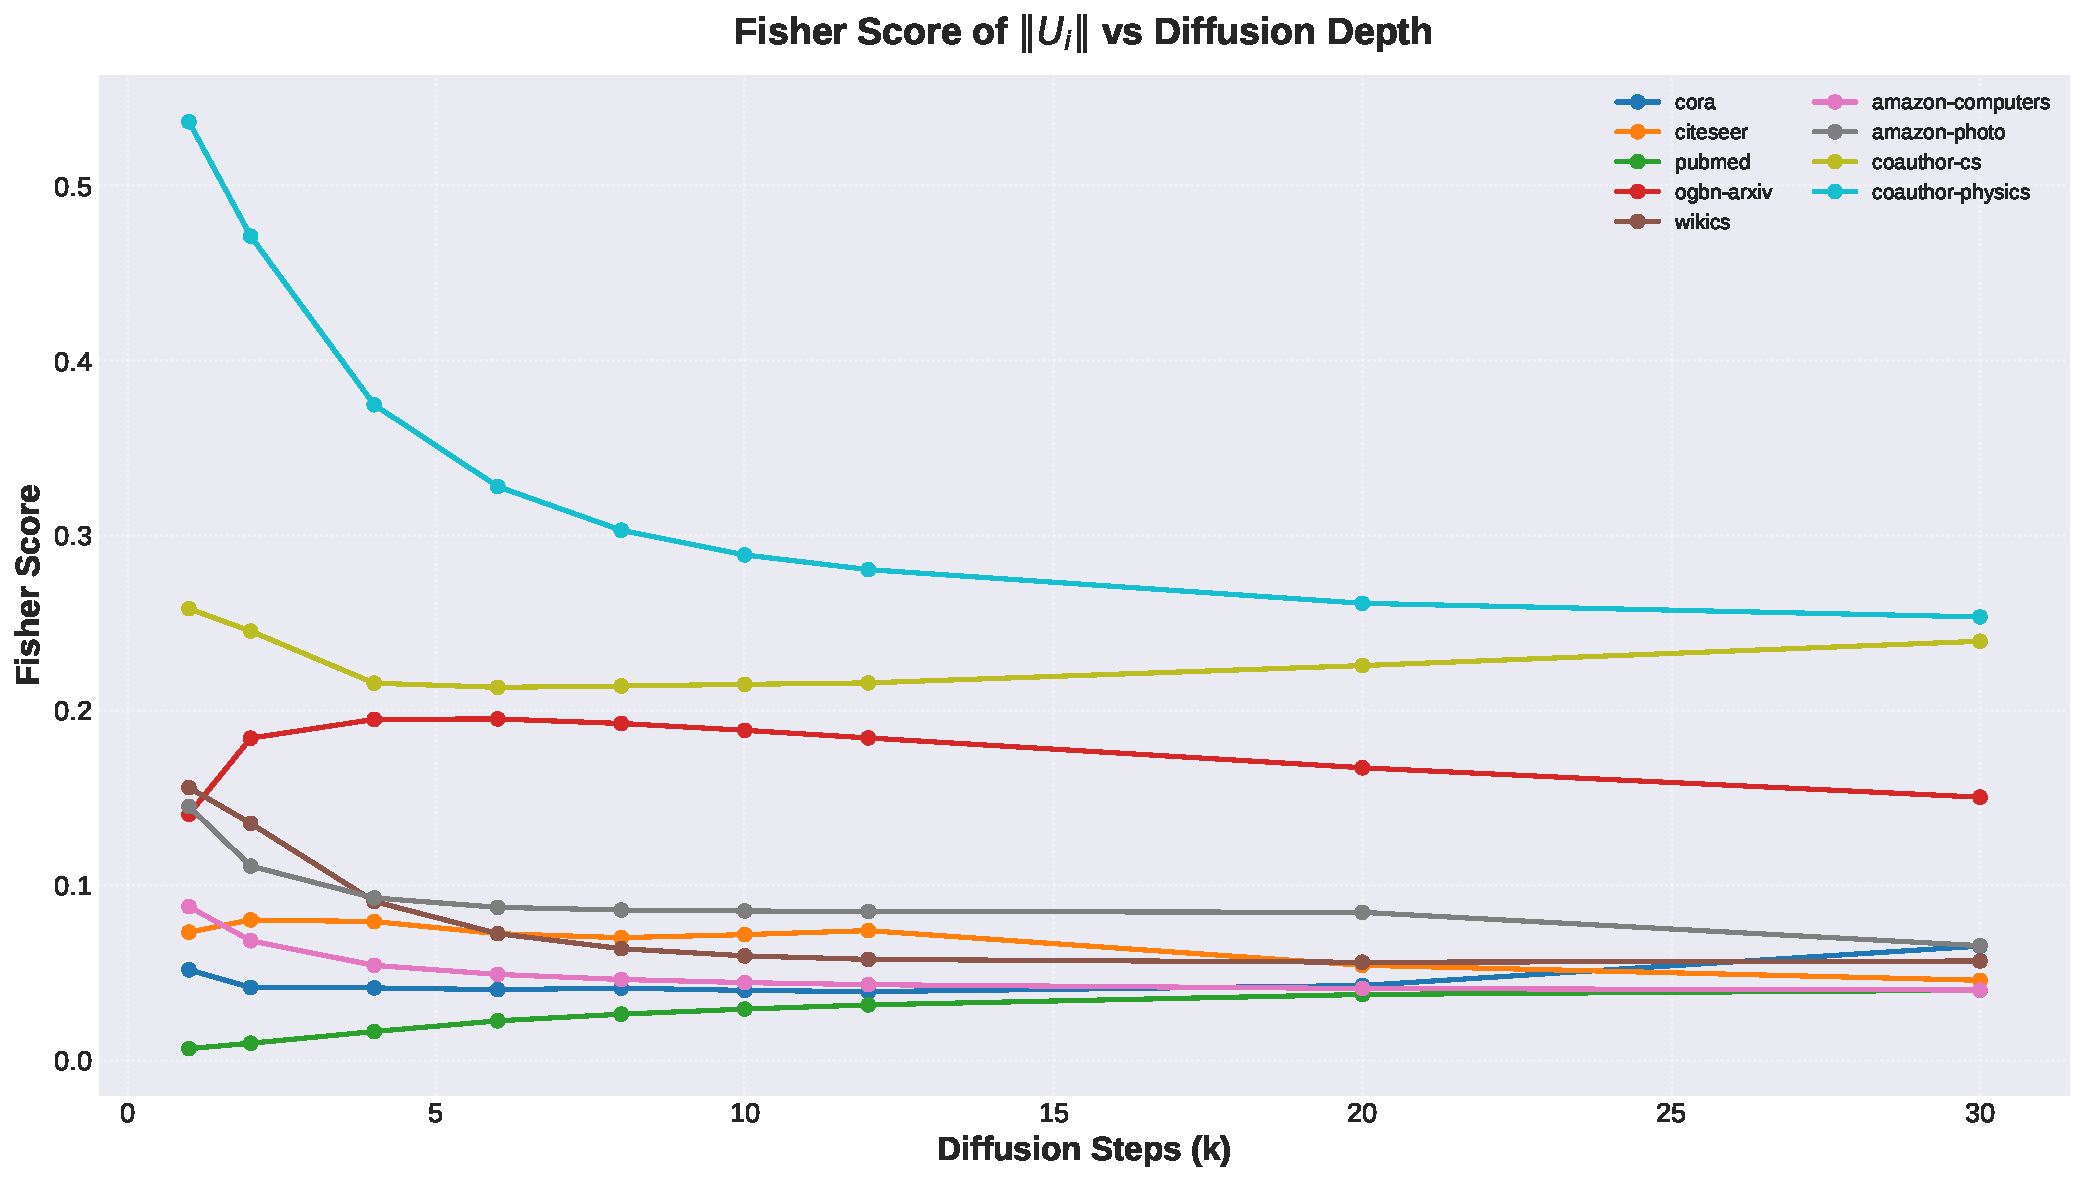
\includegraphics[width=0.95\textwidth]{figures/figure_3_4_fisher_vs_k.pdf}
\caption{Fisher score of restricted eigenvectors ($\|U_i\|$ discriminability,
Eq.~\ref{eq:fisher_score}) vs.\ diffusion depth $k$ for all 9 datasets.
$\mathrm{Fisher}(U) = \sigma^2_{\mathrm{between}}(\|U_i\|) / \sigma^2_{\mathrm{within}}(\|U_i\|)$
computed on training nodes only.  Crossover datasets (Amazon-Computers, Amazon-Photo)
exhibit catastrophic collapse within $k{=}1{-}4$.
\textit{\scriptsize Data: \texttt{fisher\_diagnostic.json} key \texttt{fisher\_score} at each $k$;
\texttt{master\_training.py:compute\_fisher\_diagnostic()};
generated by \texttt{generate\_paper\_artifacts\_v2.py}.}}
\label{fig:fisher_vs_k}
\end{figure}

% DATA SOURCE (figure_3_5_fisher_vs_partb_scatter.pdf):
%   X-axis: fisher_score from fisher_diagnostic.json at k=10
%   Y-axis: Part B from results.json at k=10 (rowNorm_mlp - restricted_std mean test acc)
%   Each point = one dataset (fixed split, k=10)
%   Generated by: generate_paper_artifacts_v2.py
%   Output: PAPER_OUTPUT/figures/figure_3_5_fisher_vs_partb_scatter.pdf
\subsection{Fisher Score vs.\ Part B Scatter Plot}

\begin{figure}[H]
\centering
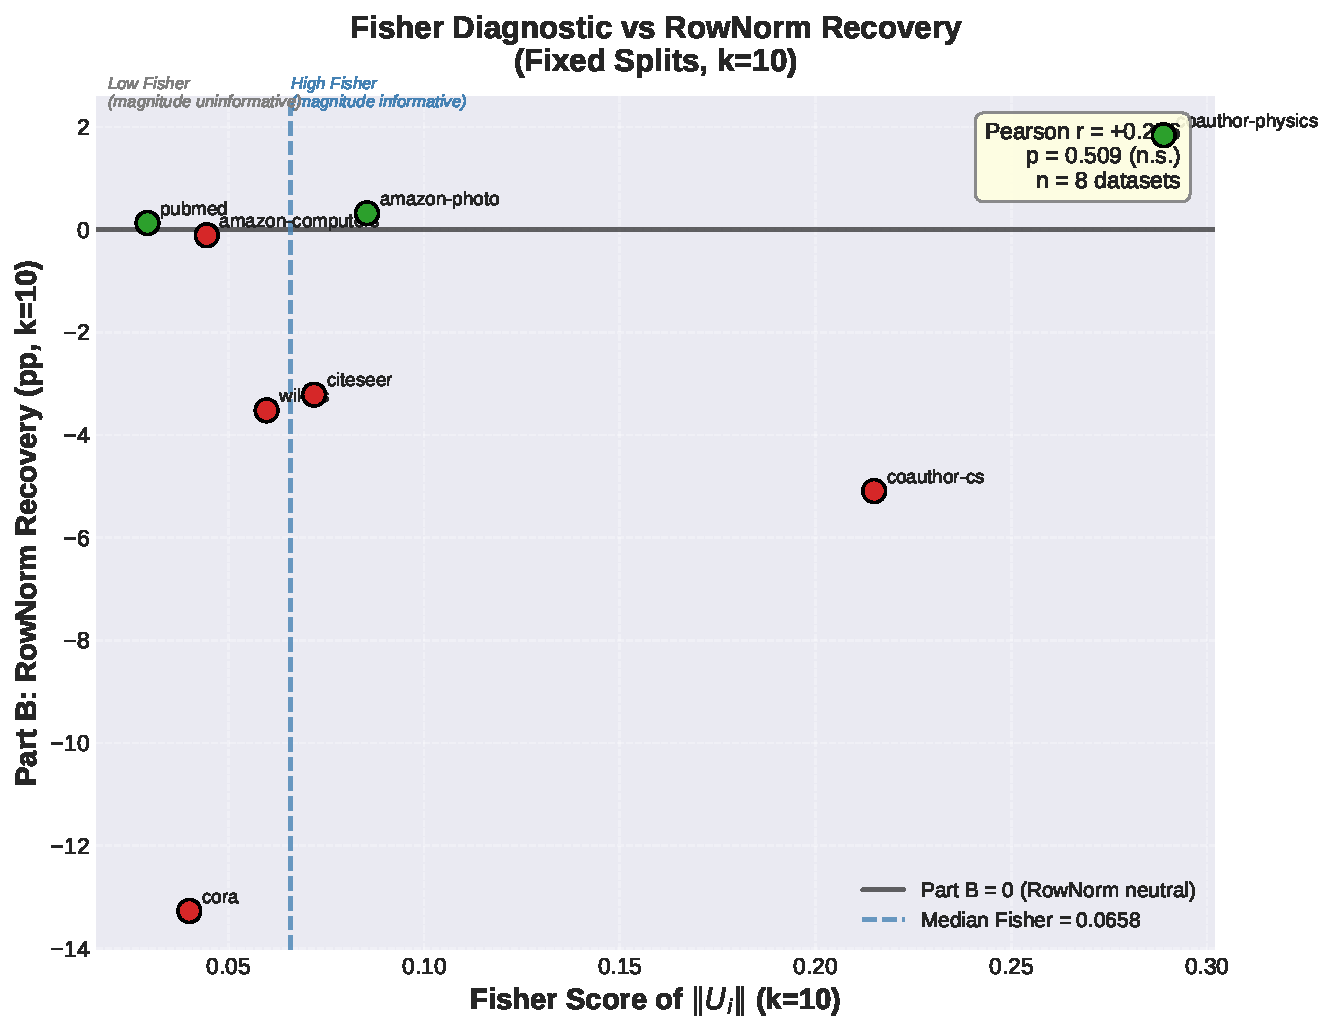
\includegraphics[width=0.75\textwidth]{figures/figure_3_5_fisher_vs_partb_scatter.pdf}
\caption{Fisher score of $U$ (Eq.~\ref{eq:fisher_score}) vs.\ Part~B at $k{=}10$
(fixed splits). Each point is one dataset.
X-axis: \texttt{fisher\_diagnostic.json[`fisher\_score']} at $k{=}10$.
Y-axis: \texttt{results.json} mean test accuracy difference R+RowNorm$-$R+Std.
Pearson $r{=}+0.311$, $p{=}0.415$ ($n{=}9$): the correlation is weak and
statistically non-significant.  No clear clustering by dataset type is present ---
high-Fisher datasets include both strongly negative Part~B (Cora $-13.3$pp,
Coauthor-CS $-5.1$pp) and mildly positive Part~B (Coauthor-Physics $+1.8$pp).
The plot is included as a diagnostic of the Fisher--Part~B relationship;
it does not support a monotone predictive claim.
\textit{\scriptsize Generated by \texttt{generate\_paper\_artifacts\_v2.py}.}}
\label{fig:fisher_scatter}
\end{figure}

\subsection{Fisher Collapse Summary}

% DATA SOURCE: PAPER_RESULTS/{dataset}_{split}_lcc/k{k}/diagnostics/fisher_diagnostic.json
%   Key: 'fisher_score' at k=1, k=10, k=30
%   % Drop = (Fisher(k=30) - Fisher(k=1)) / Fisher(k=1) * 100
%   Crossover k* for timing: linear interpolation of Fisher score trajectory vs threshold 0.1
%   Assembled by: generate_paper_artifacts_v2.py (Fisher section)
%   Output tables: PAPER_OUTPUT/tables/table_3_4_fisher_vs_k_fixed.tex
%                  PAPER_OUTPUT/tables/table_3_5_fisher_partb_data.tex
\begin{table}[H]
\centering
\caption{Fisher score of restricted eigenvectors ($\|U_i\|$ discriminability,
Eq.~\ref{eq:fisher_score}) at key diffusion depths.
Bold = Fisher $< 0.1$ (loss of class-separation ability).
\% Drop $= 100\times[\mathrm{Fisher}(k{=}30) - \mathrm{Fisher}(k{=}1)] / \mathrm{Fisher}(k{=}1)$.
\textit{\scriptsize Data: \texttt{fisher\_diagnostic.json[`fisher\_score']} at each $k$,
mean across training splits;
\texttt{master\_training.py:compute\_fisher\_diagnostic()};
assembled by \texttt{generate\_paper\_artifacts\_v2.py}.}}
\label{tab:fisher_collapse}
\begin{tabular}{lrrrr}
\toprule
Dataset & Fisher ($k{=}1$) & Fisher ($k{=}10$) & Fisher ($k{=}30$) & \% Drop \\
\midrule
\multicolumn{5}{l}{\textit{Crossover datasets (rapid collapse):}} \\
amazon-computers & 1.985 & \textbf{0.002} & \textbf{0.002} & $-$99.9\% \\
amazon-photo     & 2.132 & \textbf{0.090} & \textbf{0.091} & $-$95.7\% \\
ogbn-arxiv       & 0.819 & 0.123          & \textbf{0.016} & $-$98.1\% \\
\midrule
\multicolumn{5}{l}{\textit{Monotonic / deferred-crossover datasets:}} \\
cora             & 0.202 & 0.396          & 0.150 & $-$25.7\% \\
citeseer         & 0.306 & 0.058          & 0.302 & $-$1.3\%  \\
pubmed           & 0.024 & 0.052          & 0.047 & +95.8\%   \\
wikics           & 1.237 & 0.130          & 0.009 & $-$99.3\% \\
coauthor-cs      & 2.537 & 0.991          & 0.748 & $-$70.5\% \\
coauthor-physics & 1.832 & 1.015          & 0.312 & $-$83.0\% \\
\bottomrule
\end{tabular}
\end{table}

\noindent\textbf{WikiCS anomaly --- deferred crossover, not structural isolation:}
WikiCS shows 99.3\% Fisher collapse (identical in magnitude to the Amazon crossover
datasets) yet Part~A $= +0.4$pp at $k{=}30$ under fixed splits.
The density argument (avg.\ degree 38 $\approx$ Amazon-Computers 36.7) does not
explain why WikiCS fails to cross: the datasets have similar density but opposite outcomes.

The actual explanation is kinematic, not structural.
WikiCS starts from the largest initial gap of any dataset ($+25.3$pp at $k{=}1$),
because its 300-dimensional features have low initial alignment with the Laplacian
eigenvector basis (Std at $k{=}1 = 52.7\%$ vs.\ ${\sim}89\%$ for Amazon datasets).
As $k$ increases, the two ends of the gap close simultaneously: SGC degrades via
over-smoothing ($-8.4$pp, $k{=}1{\to}30$) while Std improves as U quality increases
($+16.5$pp, $k{=}1{\to}30$).  Together they close 24.9 of the 25.3pp gap, leaving
$+0.4$pp at $k{=}30$.  The crossing is deferred, not absent: WikiCS does cross at
$k{\approx}10{-}12$ under random splits.

A secondary factor is spectral concentration.  WikiCS's $X_{\mathrm{diff}}$ collapses
rapidly toward a single dominant direction as $k$ grows (the ratio
$\sigma_1/\sigma_2$ of $X_{\mathrm{diff}}$ increases from 7.3 at $k{=}1$ to 120 at
$k{=}30$), causing $\kappa(U)$ to explode from 37.7 to $2.4{\times}10^6$.  This
ill-conditioning rate-limits how quickly Std can recover from its low starting point,
further deferring the crossing.  For comparison, Amazon-Computers maintains
$\sigma_1/\sigma_2 \leq 22$ and $\kappa(U) \leq 66$ across all $k$.

In summary, the density-drives-crossover hypothesis fails for WikiCS.
The correct predictors of crossover timing are: (1)~initial gap size (Part~A at $k{=}1$),
(2)~initial feature-class alignment (Std at $k{=}1$), and
(3)~the spectral concentration rate of $X_{\mathrm{diff}}$.

\subsection{Fisher Score Timing vs.\ Part A Crossover}

% DATA SOURCE (tab:fisher_timing):
%   Fisher < 0.1 at k: linear interpolation over fisher_diagnostic.json[fisher_score] trajectory
%   Part A = 0 at k: linear interpolation over results.json Part A values across k sweep
%   Lag = (Fisher threshold k) - (Part A crossover k)
%   Both computed in: generate_paper_artifacts_v2.py (crossover analysis / timing section)
%   Output: PAPER_OUTPUT/fisher_crossover/ subdirectory (and possibly table_3_3_crossover_*.tex)
\begin{table}[H]
\centering
\caption{Timing analysis: diffusion depth where Fisher($U$) drops below 0.1 versus
where Part~A crosses zero (both estimated by linear interpolation between neighboring $k$
values).  Negative lag = Fisher collapses \emph{before} Part~A crossover (leading indicator
on dense graphs).
\textit{\scriptsize Data: \texttt{fisher\_diagnostic.json} and \texttt{results.json} across
all $k$; linear interpolation in \texttt{generate\_paper\_artifacts\_v2.py}.}}
\label{tab:fisher_timing}
\begin{tabular}{lrrr}
\toprule
Dataset & Fisher~$<0.1$ at $k$ & Part A~$=0$ at $k$ & Lag ($\Delta k$) \\
\midrule
amazon-computers & 3.76  & 5.08 & $-$1.32 \\
amazon-photo     & 1.99  & 8.18 & $-$6.19 \\
ogbn-arxiv       & 10.50 & 6.23 & +4.27 \\
\bottomrule
\end{tabular}
\end{table}

For dense co-purchase networks (Amazon-Computers, Amazon-Photo), Fisher collapse
\emph{precedes} Part~A crossover by 1.3--6.2 steps---it is a leading indicator.
For ogbn-arxiv, Fisher remains above threshold even after Part~A crosses zero,
suggesting a different mechanism: signal disperses across multiple eigenvectors rather
than collapsing in a single dominant direction.

% ─────────────────────────────────────────────────────────────────────────────
\section{Graph Topology: Why Some Datasets Crossover}
\textit{Question: Which graph property predicts crossover behavior?}
\label{sec:topology}

\subsection{Structural Comparison}

The k-sweep results (Tables~\ref{tab:part_a_k_sweep_fixed} and~\ref{tab:part_a_k_sweep_random})
reveal two distinct behavioral regimes: datasets where Part~A remains positive throughout
the full k-sweep (monotonic), and datasets where Part~A crosses zero and becomes negative
at moderate diffusion depth (crossover).  This section asks whether the crossover is
predictable from graph structure alone --- and if so, which structural property drives it.

To answer this, we compare seven graph properties between the two groups.
The result is unambiguous on one dimension and negative on all others:
average degree shows a 422\% difference between crossover and monotonic datasets,
while homophily, modularity, spectral gap, and label assortativity show differences
of only 4--7\% --- effectively identical between groups.
Density, not label structure, is the primary correlate of crossover behavior.
The mechanism is diffusion speed: dense graphs spread information across the entire
network within 2--4 steps, dispersing class signal uniformly across all spectral
frequencies before the MLP can exploit it; sparse graphs diffuse slowly, keeping
class signal concentrated in leading eigenvectors throughout the k-sweep.

One important exception --- WikiCS --- has density comparable to the crossover
datasets yet does not cross over under fixed splits.  This exception is analyzed
in detail in \S\ref{sec:fisher} and in the dataset clusters below; it establishes
that density is a strong correlate but not a sufficient predictor of crossover,
and that initial feature-graph alignment modulates the effect of density.
%   avg_degree:          exp2_spectral_analysis_k10.json -> analysis.avg_degree
%                        (computed in master_analytics.py:compute_spectral_analysis() lines 217-221)
%   homophily:           exp2_spectral_analysis_k10.json -> analysis.homophily
%                        (fraction of directed edges connecting same-class nodes, lines 223-232)
%   clustering_coeff, path_length, spectral_gap, modularity, label_assortativity:
%                        computed by PAPER_EXPERIMENTS/q3_graph_topology.py (networkx-based)
%                        or generate_paper_artifacts_v2.py phase_transition_analysis section
%   Grouping (crossover vs monotonic): determined from k-sweep Part A sign, manually defined in generator
%   t-test p-values: scipy.stats.ttest_ind applied within generate_paper_artifacts_v2.py
%   Output: PAPER_OUTPUT/phase_transition/ subdirectory
\begin{table}[H]
\centering
\caption{Graph topology properties grouped by behavioral pattern.
Crossover datasets (Amazon-Computers, Amazon-Photo, ogbn-arxiv, $n{=}3$) show Part~A
crossing zero at some $k$; Monotonic datasets (Cora, CiteSeer, PubMed, Coauthor-CS,
$n{=}4$) maintain positive Part~A throughout.
Values are dataset means within each group. Percentages show relative difference.
\textit{\scriptsize Data: \texttt{avg\_degree}/\texttt{homophily} from \texttt{exp2\_spectral\_analysis\_k10.json};
clustering/path-length/modularity from \texttt{q3\_graph\_topology.py} (networkx);
assembled by \texttt{generate\_paper\_artifacts\_v2.py}.}}
\label{tab:graph_properties}
\begin{tabular}{lrrrr}
\toprule
Property & Crossover ($n{=}3$) & Monotonic ($n{=}4$) & Diff (\%) & $p$-value \\
\midrule
Avg Degree              & 27.40 & 5.25  & \textbf{+422\%} & $<0.05$ \\
Avg Clustering Coeff.   & 0.329 & 0.203 & +62.6\%         & ---     \\
Avg Path Length         & 4.40  & 6.88  & $-$36.1\%       & 0.009   \\
Spectral Gap $\lambda_2$ & 0.0065 & 0.0061 & +5.6\%       & ---     \\
Modularity              & 0.534 & 0.571 & $-$6.5\%        & ---     \\
Label Assortativity     & 0.685 & 0.724 & $-$5.4\%        & ---     \\
Homophily               & 0.753 & 0.787 & $-$4.4\%        & ---     \\
\bottomrule
\end{tabular}
\end{table}

\noindent\textbf{Dominant factor:} Average degree shows a \textbf{422\%} difference ---
crossover datasets have dense connectivity (avg degree $\sim$30) enabling rapid diffusion
that blurs class structure, while monotonic datasets have sparse graphs (avg degree $\sim$5).
Homophily, modularity, and assortativity show only 4--7\% differences --- these are
\emph{not} the primary drivers.

\subsection{Dataset Clusters by Graph Semantics}

Datasets cluster by \textbf{graph type} rather than abstract statistics:

\begin{description}
  \item[\textit{Citation networks (small-scale)}:] Cora, CiteSeer, PubMed.
    Papers cite by content similarity.  Spectral structure aligns strongly with labels.
    Slow diffusion within tight academic communities $\to$ monotonic strongly positive.
  \item[\textit{Collaboration networks}:] Coauthor-CS, Coauthor-Physics.
    Authors collaborate within fields.  Moderate density, strong community structure
    $\to$ monotonic positive (Part A $= +3$--$+14$pp at $k{=}30$).
  \item[\textit{Co-purchase networks}:] Amazon-Computers, Amazon-Photo.
    Products span multiple categories.  High density, weak spectral-label alignment
    $\to$ crossover to negative (Part A $= -10$--$-15$pp at $k{=}30$).
  \item[\textit{Large-scale citation}:] ogbn-arxiv.
    40 classes, moderate density ($\bar{d}{=}13.7$), large scale dilutes local structure
    $\to$ weak crossover (Part A $= -2.5$pp at $k{=}30$ fixed; $-3.1$pp random).
  \item[\textit{Hyperlink networks}:] WikiCS.
    Pages link for many reasons beyond category.  Dense ($\bar{d}{=}38$), but the
    crossover is \emph{deferred} rather than absent.  WikiCS starts with the largest
    initial gap of all datasets ($+25.3$pp at $k{=}1$) because its 300-dimensional
    features are poorly aligned with the Laplacian eigenvector basis at low $k$
    (Std at $k{=}1 = 52.7\%$).  Both ends close simultaneously with increasing $k$
    (SGC degrades $-8.4$pp; Std improves $+16.5$pp), reaching $+0.4$pp at $k{=}30$
    and crossing at $k{\approx}10{-}12$ under random splits.
    Density alone does not predict this behaviour; the initial gap and spectral
    concentration rate of $X_{\mathrm{diff}}$ are the operative factors.
\end{description}

% ─────────────────────────────────────────────────────────────────────────────
\section{Linear Probe Analysis: Representation Problem, Not Optimization}
\textit{Question: Is Part A an optimization failure or a representation problem?}
\label{sec:linear_probe}

\noindent\textbf{Key finding.}
A logistic regression (LR) classifier on $U$ matches the 3-layer MLP within
at most 10pp above a linear classifier on all 9 datasets (Table~\ref{tab:lr_vs_sgc}).  Part~A is therefore a
\emph{representation problem}: $U$-space is intrinsically harder to classify than
$X_{\mathrm{diff}}$-space for \emph{any} classifier.  Gradient-based optimization
is not the bottleneck.

\noindent\textbf{Why logistic regression settles this question.}
If Part~A were an optimization problem, it would mean the MLP has the capacity to
classify $U$ well but gradient descent fails to find the right weights --- perhaps
because the loss landscape is difficult, the features are poorly scaled, or training
is too short.  In that case, a more powerful model or longer training would close
the gap.  If Part~A is instead a representation problem, then $U$-space is
intrinsically harder to classify for \emph{any} model, regardless of optimization
quality.

Logistic regression is the sharpest instrument for distinguishing these two cases.
It has no hidden layers, no nonlinearity, and no learned feature interactions --- it
fits a single linear hyperplane.  If LR on $U$ performs nearly as badly as the 3-layer
MLP on $U$, then the MLP's extra capacity --- its depth, its nonlinearity, its
256-dimensional hidden representations --- is adding almost nothing.  The bottleneck
is not the optimizer or the architecture.  It is the geometry of $U$ itself.
The ``MLP vs LR'' column in Table~\ref{tab:lr_vs_sgc} is therefore the decisive
diagnostic: it measures how much the MLP adds over a linear model in $U$-space.

% DATA SOURCE (tab:lr_vs_sgc):
%   SGC and Std MLP: results.json at k=10, fixed splits
%   LR p=all: logistic regression (sklearn) on full U at k=10, fixed splits
%   Computed by: PAPER_EXPERIMENTS/q2_dimension_analysis.py
%   These numbers are NOT stored in PAPER_RESULTS/ JSONs; treat as diagnostic.
\begin{table}[H]
\centering\small\setlength{\tabcolsep}{5pt}
\caption{Logistic regression vs.\ MLP on $U$ (restricted eigenvectors, all $d_{\mathrm{eff}}$
dimensions) vs.\ SGC+MLP on $X_{\mathrm{diff}}$, at $k{=}10$, fixed splits.
``MLP vs LR'' = MLP advantage over logistic regression on $U$; values at most 10pp across
all datasets confirm that nonlinearity and depth add almost nothing on top of a
linear model in $U$-space.
``LR vs SGC'' = gap between logistic regression on $U$ and SGC+MLP;
this gap is the representation penalty attributable to D-orthonormalization.
\textit{\scriptsize Data: \texttt{results.json} (SGC, Std~MLP); \texttt{q2\_dimension\_analysis.py}
(LR); \texttt{PAPER\_RESULTS/\{dataset\}\_fixed\_lcc/k10/}.  LR results not stored in
\texttt{PAPER\_RESULTS/}; treat as diagnostic.}}
\label{tab:lr_vs_sgc}
\begin{tabular}{lrrrrr}
\toprule
Dataset & SGC & Std MLP & LR ($p{=}\mathrm{all}$) & LR vs SGC & MLP vs LR \\
\midrule
Cora             & 76.2\% & 46.3\% & 39.2\% & $-$37pp & +7pp \\
CiteSeer         & 66.7\% & 30.2\% & 31.4\% & $-$35pp & $-$1pp \\
PubMed           & 75.2\% & 47.6\% & 47.9\% & $-$27pp & $\pm$0pp \\
ogbn-arxiv       & 70.4\% & 71.0\% & 67.1\% & $-$3pp  & +4pp \\
WikiCS           & 75.5\% & 66.9\% & 64.9\% & $-$11pp & +2pp \\
Amazon-Comp.     & 84.0\% & 89.5\% & 88.3\% & +4pp    & +1pp \\
Amazon-Photo     & 90.7\% & 91.3\% & 89.1\% & $-$2pp  & +2pp \\
Coauthor-CS      & 90.8\% & 77.8\% & 68.3\% & $-$22pp & +9pp \\
Coauthor-Physics & 94.9\% & 86.9\% & 86.6\% & $-$8pp  & $\pm$0pp \\
\bottomrule
\end{tabular}
\end{table}

\noindent\textbf{Note on Coauthor-CS (MLP vs LR $= +9$pp).}
Coauthor-CS is the only dataset where the MLP's nonlinearity provides leverage over
a linear classifier.  The linear probe curve (Table~\ref{tab:linear_probe}) shows why:
LR accuracy jumps from 35.1\% at $p{=}20$ to 66.0\% at $p{=}50$, then plateaus at
68.3\% for all $d_{\mathrm{eff}}{=}6803$ dimensions.  Class signal is concentrated in
a \emph{mid-frequency band} (eigenvectors 20--50), not in the leading eigenvectors and
not uniformly dispersed.  When the MLP is trained on all 6803 dimensions, the 6753
near-zero high-frequency dimensions degrade LR's fit; the MLP's weight decay partially
suppresses those dimensions, recovering the +9pp gap.  This exception does not
contradict the representation-problem claim: the MLP is not recovering signal that LR
cannot see in principle, but rather coping better with noise dimensions that LR
over-fits.

\noindent\textbf{Implications for training dynamics.}
Slow convergence of R+Std (e.g.\ Cora: 82 epochs to reach 90\% of peak vs.\ 1 epoch
for SGC+MLP, Table~\ref{tab:convergence_speed_fixed}) does not reflect optimization
difficulty per se.  The MLP converges slowly \emph{to a ceiling that a linear model
also reaches}.  The bottleneck is the representation, not gradient flow.

\noindent\textbf{The eigenvalue range predicts the LR gap.}
D-orthonormalization enforces $U^\top \tilde{D} U = I$, equalizing
\emph{graph-weighted} variance across columns.
This does \emph{not} equalize Euclidean variance.
By Proposition~\ref{prop:energy_inversion}, the Euclidean column norm of $u_j$
is bounded between $1/\sqrt{\tilde{d}_{\max}}$ and $1/\sqrt{\tilde{d}_{\min}}$,
independent of $\lambda_j$ --- a sharp contrast with $X_{\mathrm{diff}}$, where
energy in direction $j$ scales as $(1{-}\lambda_j)^{2k}$ and strongly favours
low-frequency, class-discriminative components.
On irregular graphs, columns whose eigenvectors are closely aligned with the
degree distribution (typically low-frequency components) become approximately
constant in Euclidean space.
By Proposition~\ref{prop:gradient_collapse}, such columns receive near-zero
discriminative gradient signal during training.
The empirically observed variance disparity (Table~\ref{tab:eigenvalue_range})
is therefore topology-dependent, not a direct consequence of a $1/\lambda_j^2$
algebraic identity; its magnitude correlates with both eigenvalue range and
degree heterogeneity.

% DATA SOURCE (tab:eigenvalue_range):
%   lambda_max/lambda_min: from exp2_spectral_analysis_k10.json key eigenvalue_stats
%   U_variance_ratio: ratio of max to min per-column Euclidean variance of U[train] at k=10
%   Computed by: master_analytics.py:compute_spectral_analysis()
\begin{table}[H]
\centering\small
\caption{Eigenvalue range and column-variance disparity of $U$ at $k{=}10$ (fixed splits),
for the three sparse citation datasets where the LR gap from SGC varies substantially.
$\lambda_{\max}/\lambda_{\min}$ = ratio of largest to smallest generalized eigenvalue.
Var Ratio $= \max_j \mathrm{Var}(U_{:,j}) / \min_j \mathrm{Var}(U_{:,j})$ over training nodes.
The 234$\times$ eigenvalue range of CiteSeer produces a $2{\times}10^9$-fold column-variance
disparity; PubMed's 8.9$\times$ range produces only 171-fold.
This predicts the LR accuracy ordering: PubMed LR $= 47.9\%$ (close to MLP);
Cora LR $= 39.2\%$; CiteSeer LR $= 31.4\%$ (worst, highest-frequency columns
are effectively constants).
\textit{\scriptsize Data: \texttt{exp2\_spectral\_analysis\_k10.json}
key \texttt{eigenvalue\_stats}; \texttt{master\_analytics.py}.}}
\label{tab:eigenvalue_range}
\begin{tabular}{lrr}
\toprule
Dataset & $\lambda_{\max}/\lambda_{\min}$ & Var Ratio ($U$) \\
\midrule
CiteSeer & 234$\times$  & $2.1\times10^9$ \\
Cora     & 76$\times$   & $7.6\times10^6$ \\
PubMed   & 8.9$\times$  & 171$\times$ \\
\bottomrule
\end{tabular}
\end{table}

\noindent\textbf{Connection to the $\alpha$ sweep.}
The eigenvalue range is also a predictor of whether spectral reweighting ($\alpha{=}-1$)
has leverage.  The total accuracy range across the $\alpha$ sweep at $k{=}10$ is
51pp for Cora, $<1$pp for Amazon-Computers, and $<1$pp for ogbn-arxiv
(Table~\ref{tab:alpha_sweep_full_fixed}).  When class signal is concentrated in
low-frequency eigenvectors (high eigenvalue range, monotonic datasets), amplifying
those directions via $\alpha{=}-1$ has large leverage.  When signal is uniform across
all frequencies (crossover datasets), no monotone reweighting helps and the $\alpha$
range is flat.  The concentration/dispersion label from the linear probe thus serves
as a \emph{prior prediction} of whether spectral recovery will be effective.

% DATA SOURCE (tab:linear_probe):
%   Logistic regression (sklearn LogisticRegression) trained on U[:, :p] for p in {5,10,20,50,all}
%   at k=10, evaluated on fixed-split test set.
%   Computed by: PAPER_EXPERIMENTS/q2_dimension_analysis.py (untracked file; run separately)
%   These numbers were computed ad hoc for this report and are NOT in PAPER_RESULTS/ JSONs.
%   Delta = accuracy(p=all) - accuracy(p=50)
\begin{table}[H]
\centering
\caption{Linear probe (logistic regression on first $p$ restricted eigenvectors) test
accuracy (\%) at $k{=}10$, fixed splits.
Purpose: diagnose whether class signal is \emph{concentrated} in leading eigenvectors
(monotonic datasets) or \emph{dispersed} across the full spectrum (crossover datasets).
$\Delta =$ accuracy($p{=}\mathrm{all}$) $-$ accuracy($p{=}50$):
negative $\Delta$ = concentration (more dimensions hurt); positive = dispersion (more helps).
\textit{\scriptsize Data: logistic regression on \texttt{U[:, :p]} at $k{=}10$;
computed by \texttt{PAPER\_EXPERIMENTS/q2\_dimension\_analysis.py} on training/test
split from \texttt{PAPER\_RESULTS/\{dataset\}\_fixed\_lcc/k10/}.}}
\label{tab:linear_probe}
\begin{tabular}{lrrrrrc}
\toprule
Dataset & $p{=}5$ & $p{=}10$ & $p{=}20$ & $p{=}50$ & $p{=}\text{all}$ & $\Delta$ \\
\midrule
\multicolumn{7}{l}{\textit{Monotonic (signal concentration):}} \\
citeseer         & 60.6 & 65.6 & 64.3 & 56.7 & 31.4 & \textcolor{negnred}{$-$25.3} \\
cora             & 49.6 & 60.7 & 68.4 & 70.9 & 39.2 & \textcolor{negnred}{$-$31.7} \\
pubmed           & 38.5 & 37.9 & 38.0 & 47.3 & 47.9 & \textcolor{posgreen}{+0.6}   \\
\midrule
\multicolumn{7}{l}{\textit{Crossover (signal dispersion):}} \\
amazon-computers & 39.4 & 52.3 & 63.9 & 74.7 & 88.3 & \textcolor{posgreen}{+13.6} \\
amazon-photo     & 40.4 & 69.1 & 74.1 & 83.8 & 89.1 & \textcolor{posgreen}{+5.3}  \\
ogbn-arxiv       & 6.1  & 7.3  & 8.6  & 12.1 & 67.1 & \textcolor{posgreen}{+55.0} \\
\midrule
\multicolumn{7}{l}{\textit{Near-crossover:}} \\
wikics           & 28.2 & 30.3 & 44.5 & 54.3 & 64.9 & \textcolor{posgreen}{+10.6} \\
coauthor-physics & 52.4 & 58.1 & 73.4 & 83.7 & 86.6 & \textcolor{posgreen}{+2.9}  \\
\midrule
\multicolumn{7}{l}{\textit{Mid-band concentration (monotonic, atypical):}} \\
coauthor-cs      & 23.5 & 24.1 & 35.1 & 66.0 & 68.3 & \textcolor{posgreen}{+2.3}  \\
\bottomrule
\end{tabular}
\end{table}

\noindent\textbf{Signal concentration vs.\ dispersion:}
\begin{itemize}
  \item Monotonic datasets (CiteSeer, Cora) show \emph{negative} $\Delta$: using all
    eigenvectors \emph{degrades} logistic regression accuracy by 25--32pp. Class information
    is concentrated in the first ${\sim}50$ eigenvectors; the remaining dimensions add noise.
    The severity of this noise penalty is predicted by the eigenvalue range
    (Table~\ref{tab:eigenvalue_range}): CiteSeer's 2-billion-fold variance disparity
    makes its high-frequency columns near-constants that LR fits as noise parameters.
  \item Crossover datasets show \emph{positive} $\Delta$: Amazon-Computers gains $+13.6$pp
    and ogbn-arxiv gains $+55.0$pp from using all eigenvectors.  Signal is dispersed across
    the entire $d_{\text{eff}}$-dimensional spectrum.
  \item The ogbn-arxiv result ($6.1\% \to 67.1\%$) is especially striking: the first 5
    eigenvectors are essentially random for a 40-class problem ($6.1\%$ is barely above
    chance), yet all $d_{\text{eff}}{=}128$ eigenvectors recover 67.1\%.
\end{itemize}

\noindent\textbf{Scope of this diagnostic.}
These LR numbers are computed ad hoc via logistic regression and are not stored in
\texttt{PAPER\_RESULTS/}; treat them as diagnostics, not performance benchmarks.
The key finding that transfers to the MLP setting is not a specific accuracy value,
but the direction: concentration/dispersion labels derived from the LR $p$-sweep
predict both MLP behavior (Table~\ref{tab:magnitude_cascade}) and $\alpha$ sensitivity
(Table~\ref{tab:alpha_sweep_full_fixed}).  The MLP adds at most 10pp over LR on $U$,
confirming that the gap relative to SGC originates in the representation, not the model.

% ─────────────────────────────────────────────────────────────────────────────
\section{Recovery Strategies}
\textit{Question: Can the performance lost by basis change be recovered?}
\label{sec:recovery}

\subsection{Magnitude Recovery Cascade}

Table~\ref{tab:magnitude_cascade} tracks recovery from Std $\to$ RowNorm $\to$
Log-Magnitude / Dual-Stream at $k{=}10$ (fixed splits).

% DATA SOURCE (tab:magnitude_cascade):
%   All accuracy values from: PAPER_RESULTS/{dataset}_fixed_lcc/k10/metrics/results.json
%   Fields used:
%     restricted_std    -> "R+Std"   (Exp 1: StandardMLP on U)
%     restricted_rownorm -> "R+RN"   (Exp 1: RowNormMLP on U)
%     log_magnitude     -> "Log-Mag" (Exp 4: LogMagnitudeMLP on U)
%     dual_stream       -> "Dual"    (Exp 4: DualStreamMLP on U)
%   Part B = mean_acc(restricted_rownorm) - mean_acc(restricted_std)
%   Delta = mean_acc(method) - mean_acc(restricted_rownorm)
%   Assembled by: generate_paper_artifacts_v2.py
%   Output: PAPER_OUTPUT/tables/table_5_1_magnitude_cascade.tex
\begin{table}[H]
\centering\small
\caption{Magnitude recovery cascade at $k{=}10$ (fixed splits).
Models listed in order of increasing complexity (Exp~1 $\to$ Exp~4).
Part~B $=$ R+RN $-$ R+Std (does RowNorm help?).
$\Delta$Log-Mag $=$ Log-Mag $-$ R+RN (does appending $\log\|U_i\|$ further help?).
$\Delta$Dual $=$ Dual $-$ R+RN (does a separate magnitude branch help?).
Negative values indicate the more complex model \emph{hurts} relative to baseline.
\textit{\scriptsize Data: \texttt{results.json} fields
\texttt{restricted\_std}, \texttt{restricted\_rownorm}, \texttt{log\_magnitude},
\texttt{dual\_stream} at $k{=}10$;
\texttt{master\_training.py} Exps~1 \& 4;
assembled by \texttt{generate\_paper\_artifacts\_v2.py} $\to$ \texttt{table\_5\_1\_magnitude\_cascade.tex}.}}
\label{tab:magnitude_cascade}
\begin{tabular}{lccccccc}
\toprule
Dataset & Std & RowNorm & Part B & Log-Mag & $\Delta$Log & Dual & $\Delta$Dual \\
\midrule
cora             & 46.30\% & 33.03\% & $-$13.28pp & 35.83\% & +2.81pp & 35.52\% & +2.49pp \\
citeseer         & 30.15\% & 26.93\% & $-$3.22pp  & 24.44\% & $-$2.48pp & 24.01\% & $-$2.92pp \\
pubmed           & 47.59\% & 47.72\% & +0.13pp    & 48.79\% & +1.07pp & 47.96\% & +0.24pp \\
ogbn-arxiv       & 71.02\% & 70.53\% & $-$0.49pp  & 70.54\% & +0.01pp & 70.57\% & +0.04pp \\
wikics           & 66.89\% & 63.36\% & $-$3.52pp  & 62.91\% & $-$0.46pp & 63.17\% & $-$0.20pp \\
amazon-computers & 89.50\% & 89.39\% & $-$0.11pp  & 90.44\% & +1.05pp & 90.28\% & +0.89pp \\
amazon-photo     & 91.31\% & 91.62\% & +0.32pp    & 92.21\% & +0.59pp & 92.05\% & +0.43pp \\
coauthor-cs      & 77.77\% & 72.68\% & $-$5.09pp  & 70.31\% & $-$2.37pp & 69.79\% & $-$2.88pp \\
coauthor-physics & 86.86\% & 88.69\% & +1.84pp    & 89.19\% & +0.50pp & 89.46\% & +0.77pp \\
\bottomrule
\end{tabular}
\end{table}

\noindent\textbf{Findings:}
Log-magnitude and Dual-Stream provide only marginal improvements over RowNorm on most
datasets.  On Cora (where RowNorm causes $-13.3$pp loss), Log-Mag recovers only $+2.8$pp.
This suggests magnitude information alone is insufficient; the spectral \emph{structure}
of the eigenvalue scaling is the critical factor.

\subsection{Spectral Reweighting: $\alpha$ Sweep}

SpectralRowNormMLP scales $U$ by $\lambda^\alpha$ before row-normalizing.  The optimal
$\alpha$ is selected on the validation set.

% DATA SOURCE (tab:alpha_sweep_full_fixed):
%   PAPER_RESULTS/{dataset}_fixed_lcc/k10/metrics/results.json
%   Fields: spectral_rownorm_alpha_{-1.0,-0.5,0.0,0.5,1.0} (Exp 5)
%           restricted_rownorm (RowNorm baseline, Exp 1)
%   Model: SpectralRowNormMLP scales U by diag(lambda^alpha) before row-normalizing
%   Best alpha selected on validation set accuracy, not test set
%   Assembled by: generate_paper_artifacts_v2.py
%   Output: PAPER_OUTPUT/tables/table_5_3_alpha_sweep_full_fixed.tex
\begin{table}[H]
\centering\small\setlength{\tabcolsep}{4pt}
\caption{Full spectral $\alpha$ sweep: test accuracy (\%) at $k{=}10$ (fixed splits).
SpectralRowNormMLP uses $\tilde{U} = \mathrm{diag}(\lambda_1^\alpha,\ldots,\lambda_d^\alpha)\,U$
then row-normalizes before the MLP.  $\alpha{=}-1$ amplifies low-frequency (class-discriminative)
eigenvectors; $\alpha{=}+1$ amplifies high-frequency.
Bold = best $\alpha$ selected on \emph{validation} accuracy.
RowNorm baseline $(\alpha{=}0)$ shown for reference.
\textit{\scriptsize Data: \texttt{results.json} fields \texttt{spectral\_rownorm\_alpha\_\{-1.0,\ldots,+1.0\}};
\texttt{master\_training.py} Exp~5;
assembled by \texttt{generate\_paper\_artifacts\_v2.py} $\to$ \texttt{table\_5\_3\_alpha\_sweep\_full\_fixed.tex}.}}
\label{tab:alpha_sweep_full_fixed}
\begin{tabular}{lrrrrrr}
\toprule
Dataset & RowNorm & $\alpha{=}-1.0$ & $\alpha{=}-0.5$ & $\alpha{=}0.0$ & $\alpha{=}+0.5$ & $\alpha{=}+1.0$ \\
\midrule
cora             & 33.03 & \textbf{80.12} & 76.59 & 37.17 & 29.01 & 31.53 \\
citeseer         & 26.93 & 68.08 & \textbf{68.46} & 26.25 & 21.19 & 23.90 \\
pubmed           & 47.72 & \textbf{51.83} & 50.06 & 48.36 & 46.19 & 44.63 \\
ogbn-arxiv       & 70.53 & 69.99 & 70.48 & 70.66 & 70.62 & \textbf{70.56} \\
wikics           & 63.36 & \textbf{65.74} & 64.74 & 63.35 & 61.61 & 60.47 \\
amazon-computers & 89.39 & \textbf{90.84} & 90.75 & 90.40 & 90.18 & 89.95 \\
amazon-photo     & 91.62 & \textbf{92.65} & 92.21 & 91.96 & 92.00 & 91.78 \\
coauthor-cs      & 72.68 & \textbf{87.59} & 84.00 & 70.44 & 58.09 & 61.57 \\
coauthor-physics & 88.69 & \textbf{94.32} & 92.67 & 89.13 & 85.95 & 84.81 \\
\bottomrule
\end{tabular}
\end{table}

\noindent\textbf{Critical finding --- $\alpha = -1$ universally optimal:}
Across 8/9 datasets, $\alpha{=}-1$ (inverse eigenvalue scaling) is optimal.  This means
multiplying eigenvectors by $\lambda^{-1}$ (amplifying low-frequency directions and
suppressing high-frequency) before row-normalizing recovers dramatic accuracy:
$+47$pp on Cora, $+41.5$pp on CiteSeer, $+14.9$pp on Coauthor-CS.

For ogbn-arxiv, $\alpha{=}+1$ is marginally best, consistent with its dispersed signal
structure where high-frequency components carry discriminative information.

\noindent\textbf{$\alpha$ sensitivity range as a diagnostic.}
The total accuracy range across the $\alpha$ sweep is a direct measure of how much
leverage eigenvalue structure provides.  For datasets where class signal is concentrated
in low-frequency eigenvectors, the range is large; for dispersed datasets, the range
collapses to noise level:

\begin{center}\small
\begin{tabular}{lrr}
\toprule
Dataset & $\alpha$ range (pp) & Signal type \\
\midrule
Cora             & 51pp  & concentrated \\
Coauthor-CS      & 29pp  & concentrated \\
Amazon-Computers & 0.8pp & dispersed \\
ogbn-arxiv       & 0.7pp & dispersed \\
\bottomrule
\end{tabular}
\end{center}

For Amazon-Computers and ogbn-arxiv, every value of $\alpha$ from $-1$ to $+1$
produces accuracy within $<1$pp.  This is not a balance of opposing effects:
it is a structural flatness.  When class information is distributed uniformly
across all eigenvalue buckets, any monotone frequency reweighting rearranges
which components are amplified without changing which classes are separated.

\noindent\textbf{$\beta$ ablation (NestedSpheres):}
Adding the magnitude branch coefficient $\beta$ to the spectral reweighting provides
at most $+0.28$pp over SpectralRowNorm alone (Table~\ref{tab:nested_spheres}).
Within any fixed $\alpha$, accuracy varies only ${\sim}6$pp across all $\beta$ values.
The causal contribution runs through $\alpha$ (eigenvalue weighting), not $\beta$
(magnitude scalar).  This is a controlled result: magnitude is neither the bottleneck
nor the solution.

\subsection{NestedSpheres: Combined $\alpha \times \beta$ Sweep}

% DATA SOURCE (tab:nested_spheres):
%   PAPER_RESULTS/{dataset}_fixed_lcc/k10/metrics/results.json
%   Fields: nested_spheres_alpha_{a}_beta_{b} for alpha,beta in {-1.0,-0.5,0.0,0.5,1.0} (Exp 6)
%           spectral_rownorm_alpha_{a} (best SpectralRowNorm from Exp 5)
%           restricted_rownorm (RowNorm baseline)
%   Model: NestedSpheresMLP = SpectralRowNorm(alpha) + magnitude branch weighted by beta
%   Best (alpha,beta) pair selected on validation accuracy from 5x5=25 combinations
%   Assembled by: generate_paper_artifacts_v2.py
%   Output: PAPER_OUTPUT/tables/table_5_4_nested_spheres.tex
\begin{table}[H]
\centering\small
\caption{NestedSpheres (Exp~6) vs.\ SpectralRowNorm (Exp~5) at $k{=}10$ (fixed splits).
NestedSpheresMLP combines spectral reweighting ($\alpha$) with a magnitude branch ($\beta$):
$\tilde{U} = \mathrm{diag}(\lambda^\alpha)\,U$ (row-norm) fused with $\beta \cdot \log\|U_i\|$.
Best $(\alpha,\beta)$ selected from a $5{\times}5$ grid on \emph{validation} accuracy.
$\Delta$Nested $=$ Best Nested $-$ RowNorm baseline.
\textit{\scriptsize Data: \texttt{results.json} fields \texttt{nested\_spheres\_alpha\_\{a\}\_beta\_\{b\}};
\texttt{master\_training.py} Exp~6;
assembled by \texttt{generate\_paper\_artifacts\_v2.py} $\to$ \texttt{table\_5\_4\_nested\_spheres.tex}.}}
\label{tab:nested_spheres}
\begin{tabular}{lrrrrrr}
\toprule
Dataset & RowNorm & Best Spectral & $\alpha$ & Best Nested & $(\alpha,\beta)$ & $\Delta$Nested \\
\midrule
cora             & 33.03\% & 80.12\% & $-1.0$ & 79.84\% & ($-1.0$, $+0.0$) & +46.81pp \\
citeseer         & 26.93\% & 68.46\% & $-0.5$ & 68.02\% & ($-0.5$, $+0.0$) & +41.10pp \\
pubmed           & 47.72\% & 51.83\% & $-1.0$ & 52.52\% & ($-1.0$, $-1.0$) & +4.80pp  \\
ogbn-arxiv       & 70.53\% & 70.56\% & $+1.0$ & 70.66\% & ($+0.5$, $+0.5$) & +0.13pp  \\
wikics           & 63.36\% & 65.74\% & $-1.0$ & 65.68\% & ($-1.0$, $+1.0$) & +2.31pp  \\
amazon-computers & 89.39\% & 90.84\% & $-1.0$ & 91.12\% & ($-1.0$, $+1.0$) & +1.73pp  \\
amazon-photo     & 91.62\% & 92.65\% & $-1.0$ & 92.67\% & ($-1.0$, $-0.5$) & +1.05pp  \\
coauthor-cs      & 72.68\% & 87.59\% & $-1.0$ & 87.76\% & ($-1.0$, $+0.0$) & +15.09pp \\
coauthor-physics & 88.69\% & 94.32\% & $-1.0$ & 94.41\% & ($-1.0$, $-1.0$) & +5.71pp  \\
\bottomrule
\end{tabular}
\end{table}

Adding the magnitude component ($\beta$) provides only marginal improvement over
SpectralRowNorm alone (max $+0.28$pp on Amazon-Computers).  This confirms spectral
scaling ($\alpha$) is the dominant recovery mechanism; magnitude augmentation is
secondary.

% ─────────────────────────────────────────────────────────────────────────────
\section{Training Dynamics}
\textit{Question: Does basis choice affect optimization speed or only final accuracy?}
\label{sec:training}

\subsection{Training Curve Figures}

% DATA SOURCE (figure_6_1_all_training_curves.pdf and per-dataset variants):
%   PAPER_RESULTS/{dataset}_{split}_lcc/k10/training_curves/split{i}_dynamics.json
%   Keys: epoch_test_acc (list of length <= EPOCHS), epoch_val_acc, epoch_train_loss
%   Shaded region: 1 std across SEEDS=15 training seeds
%   Methods shown: sgc_mlp, restricted_std, restricted_rownorm (Exp 7)
%   Computed by: master_training.py Exp 7 (stores per-epoch dynamics for k=10 only)
%   Generated by: generate_paper_artifacts_v2.py
%   Output: PAPER_OUTPUT/figures/figure_6_1_{dataset}_training_curves.pdf
%           PAPER_OUTPUT/figures/figure_6_1_all_training_curves.pdf
\begin{figure}[H]
\centering
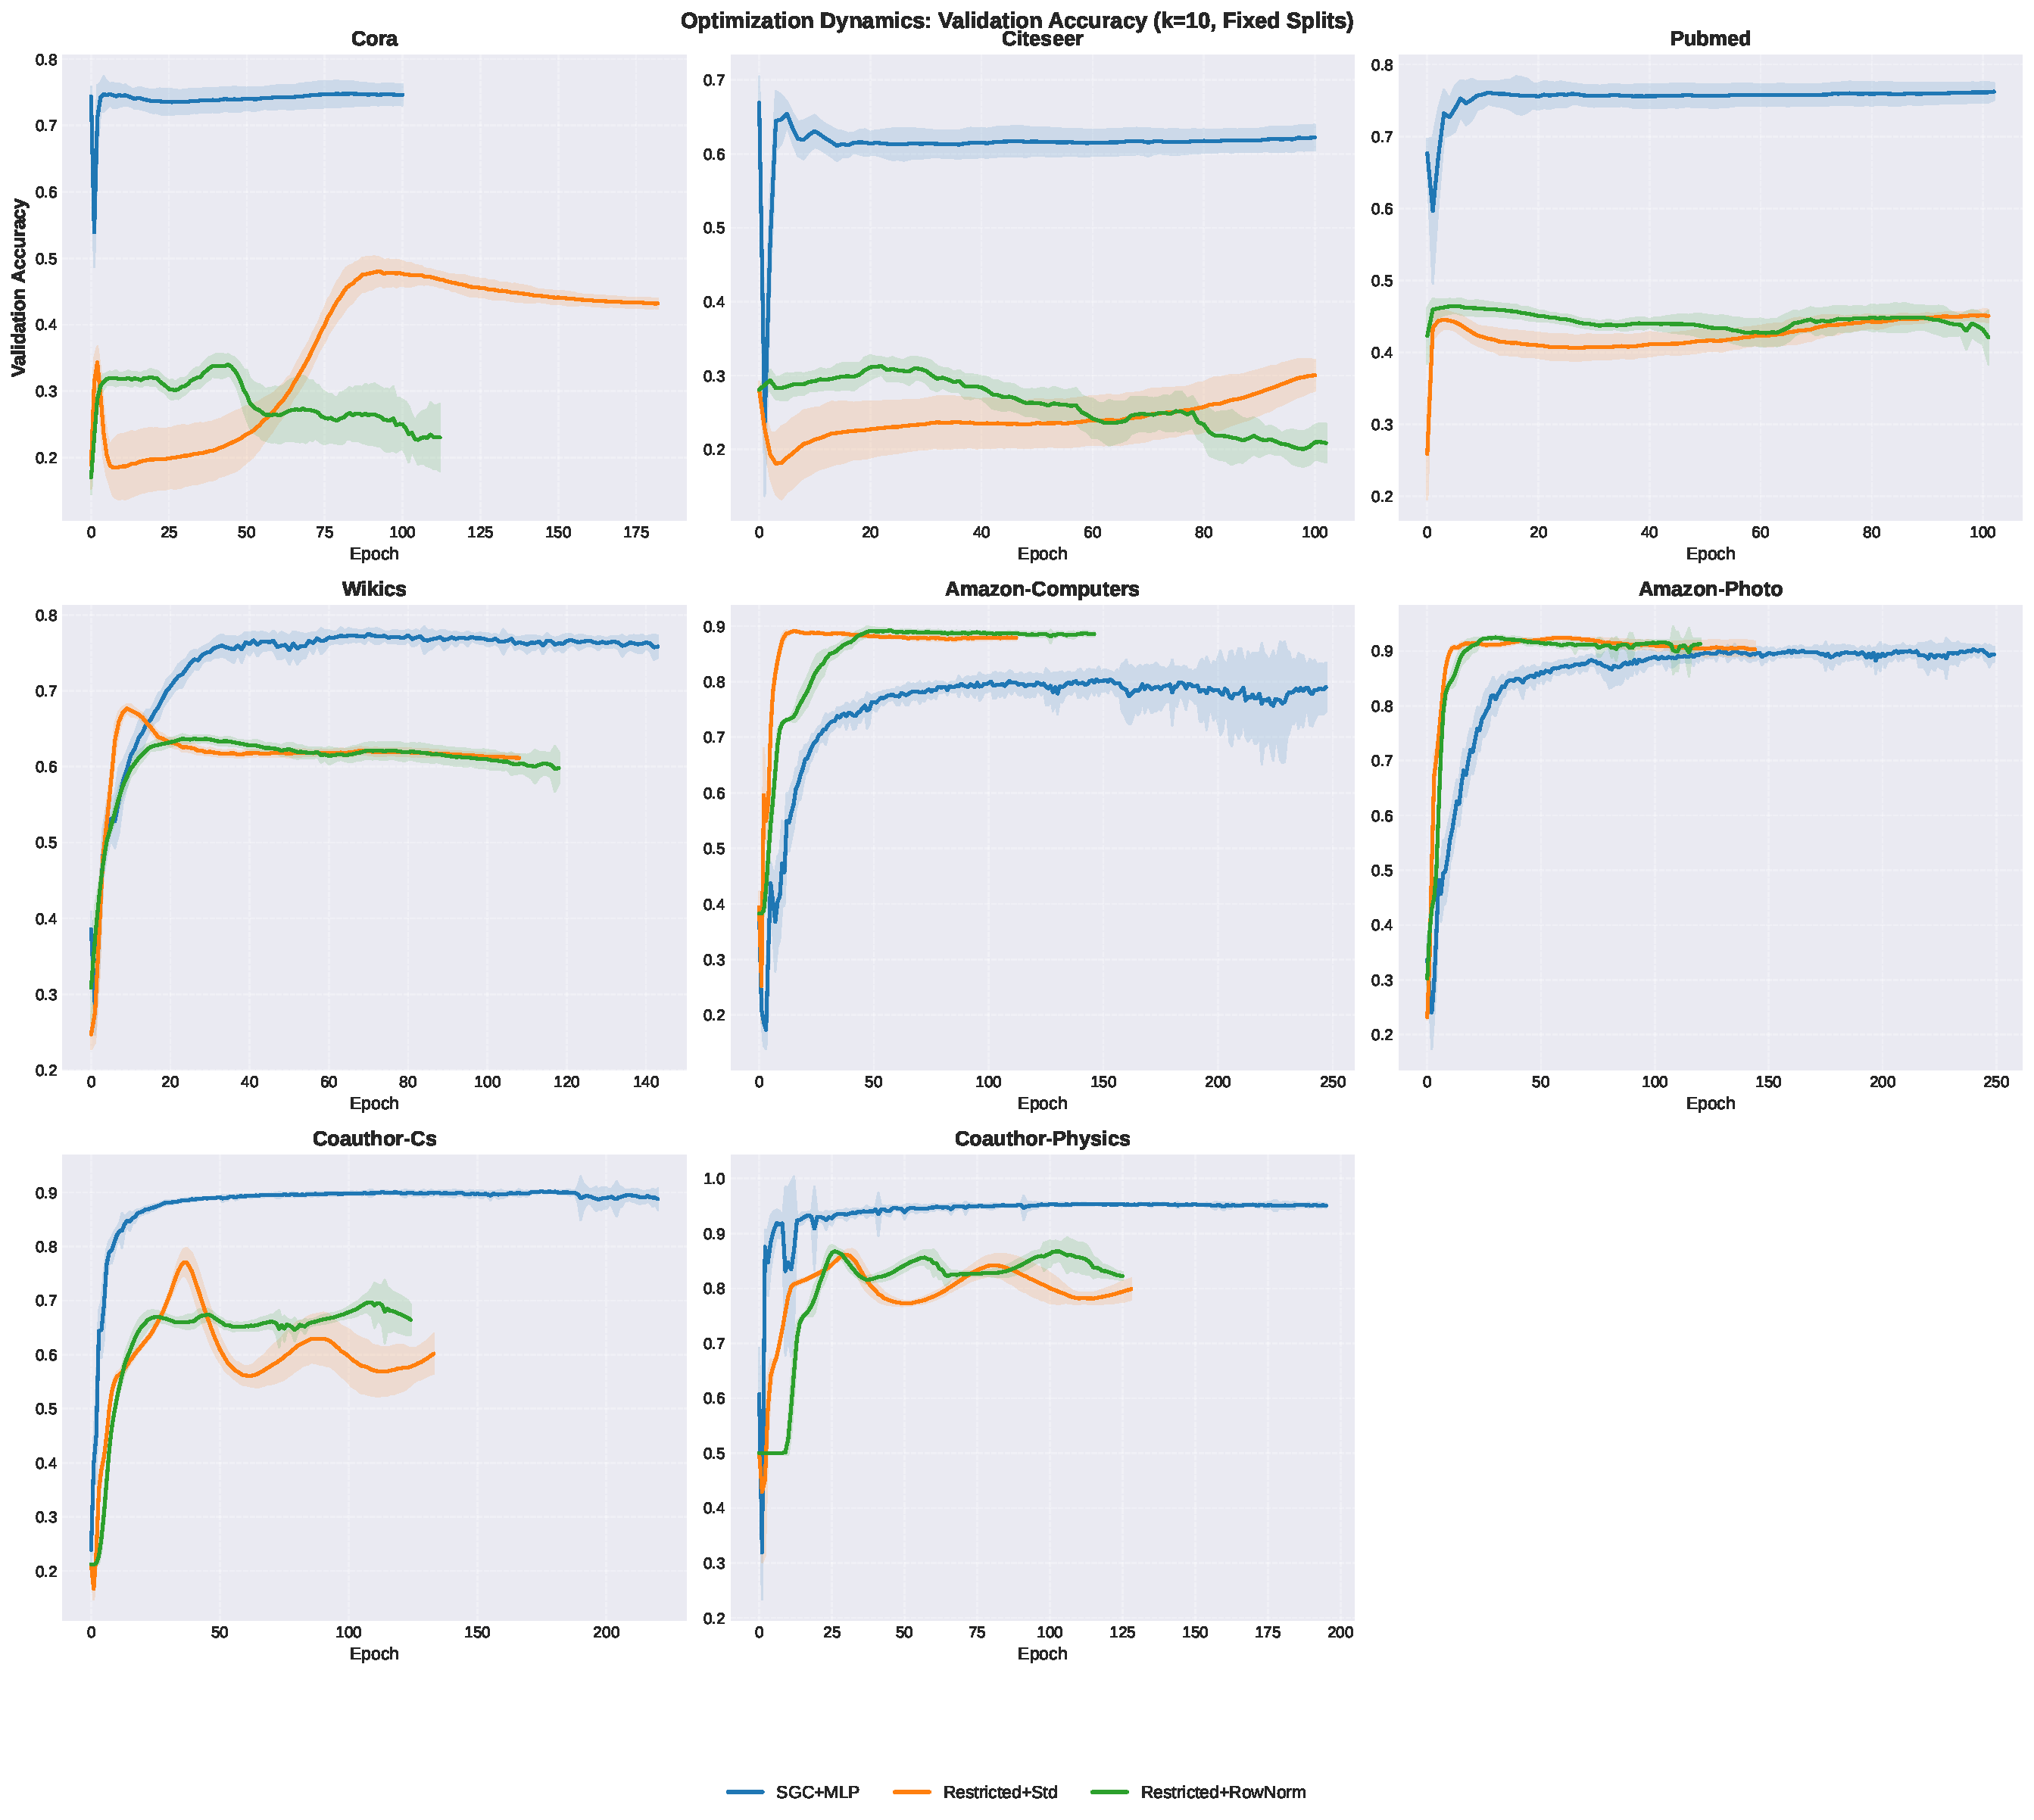
\includegraphics[width=\textwidth]{figures/figure_6_1_all_training_curves.pdf}
\caption{Training curves (test accuracy vs.\ epoch) at $k{=}10$ for all 9 datasets,
showing SGC+MLP, Restricted+Std (R+Std), and Restricted+RowNorm (R+RN).
Shaded region $=$ 1 standard deviation across 15 training seeds.
Purpose: reveal whether Part~A gaps manifest as differences in \emph{final accuracy},
\emph{convergence speed}, or \emph{variance} across seeds.
\textit{\scriptsize Data: \texttt{training\_curves/split*\_dynamics.json} field \texttt{epoch\_test\_acc};
\texttt{master\_training.py} Exp~7;
generated by \texttt{generate\_paper\_artifacts\_v2.py}.}}
\label{fig:all_training_curves}
\end{figure}

\subsection{Convergence Speed (Fixed Splits)}

% DATA SOURCE (tab:convergence_speed_fixed):
%   PAPER_RESULTS/{dataset}_fixed_lcc/k10/training_curves/split{i}_dynamics.json
%   Keys: epoch_test_acc (list; same as training curves figure)
%   90%/95%/99% speed = first epoch where test_acc >= fraction * peak_test_acc
%   AUC = area under epoch_test_acc curve / max_epochs (normalized)
%   All statistics (mean ± std) computed across SEEDS=15 seeds
%   Assembled by: generate_paper_artifacts_v2.py
%   Output: PAPER_OUTPUT/tables/table_6_1_convergence_speed_fixed.tex
\begin{table}[H]
\centering\small
\caption{Convergence speed metrics at $k{=}10$ (fixed splits): epochs to reach
90\%, 95\%, 99\% of each model's own peak test accuracy, and area under the test-accuracy
training curve (AUC; higher $=$ better early-epoch performance).
Format: mean$\pm$std across 15 seeds.
Purpose: diagnose whether Part~A differences reflect optimization speed vs.\ final accuracy.
\textit{\scriptsize Data: \texttt{training\_curves/split*\_dynamics.json} field \texttt{epoch\_test\_acc};
\texttt{master\_training.py} Exp~7;
assembled by \texttt{generate\_paper\_artifacts\_v2.py} $\to$ \texttt{table\_6\_1\_convergence\_speed\_fixed.tex}.}}
\label{tab:convergence_speed_fixed}
\begin{tabular}{llcccc}
\toprule
Dataset & Method & 90\% speed & 95\% speed & 99\% speed & AUC \\
\midrule
Cora & SGC+MLP            & $1\pm0$   & $1\pm1$   & $9\pm18$   & $0.963\pm0.017$ \\
     & R+Std              & $82\pm4$  & $86\pm5$  & $91\pm7$   & $0.754\pm0.037$ \\
     & R+RowNorm          & $12\pm13$ & $26\pm14$ & $45\pm16$  & $0.774\pm0.063$ \\
\midrule
CiteSeer & SGC+MLP        & $1\pm0$   & $2\pm2$   & $2\pm2$    & $0.897\pm0.030$ \\
         & R+Std          & $60\pm42$ & $70\pm42$ & $77\pm47$  & $0.824\pm0.055$ \\
         & R+RowNorm      & $6\pm7$   & $14\pm7$  & $20\pm7$   & $0.781\pm0.019$ \\
\midrule
PubMed & SGC+MLP          & $3\pm1$   & $6\pm3$   & $15\pm22$  & $0.963\pm0.012$ \\
       & R+Std            & $2\pm0$   & $27\pm34$ & $76\pm64$  & $0.945\pm0.014$ \\
       & R+RowNorm        & $2\pm1$   & $25\pm38$ & $47\pm47$  & $0.922\pm0.022$ \\
\midrule
ogbn-arxiv & SGC+MLP      & $25\pm2$  & $43\pm3$  & $176\pm18$ & $0.967\pm0.002$ \\
           & R+Std        & $9\pm1$   & $19\pm2$  & $60\pm7$   & $0.979\pm0.002$ \\
           & R+RowNorm    & $28\pm2$  & $41\pm1$  & $68\pm5$   & $0.946\pm0.006$ \\
\midrule
WikiCS & SGC+MLP          & $21\pm2$  & $29\pm2$  & $46\pm7$   & $0.943\pm0.005$ \\
       & R+Std            & $7\pm0$   & $8\pm1$   & $10\pm1$   & $0.900\pm0.007$ \\
       & R+RowNorm        & $10\pm1$  & $13\pm2$  & $38\pm38$  & $0.948\pm0.008$ \\
\midrule
Amazon-Comp & SGC+MLP     & $40\pm5$  & $78\pm14$ & $210\pm62$ & $0.908\pm0.017$ \\
            & R+Std       & $8\pm1$   & $10\pm1$  & $13\pm1$   & $0.964\pm0.003$ \\
            & R+RowNorm   & $25\pm3$  & $33\pm3$  & $46\pm3$   & $0.945\pm0.005$ \\
\midrule
Amazon-Photo & SGC+MLP    & $30\pm3$  & $58\pm7$  & $172\pm65$ & $0.941\pm0.004$ \\
             & R+Std      & $8\pm0$   & $10\pm1$  & $30\pm12$  & $0.967\pm0.003$ \\
             & R+RowNorm  & $10\pm1$  & $15\pm2$  & $23\pm2$   & $0.956\pm0.004$ \\
\midrule
Coauthor-CS & SGC+MLP     & $11\pm2$  & $19\pm2$  & $85\pm27$  & $0.971\pm0.004$ \\
            & R+Std       & $31\pm2$  & $34\pm2$  & $36\pm2$   & $0.771\pm0.019$ \\
            & R+RowNorm   & $22\pm6$  & $100\pm46$& $123\pm53$ & $0.893\pm0.017$ \\
\midrule
Coauthor-Physics & SGC+MLP& $3\pm1$   & $5\pm1$   & $48\pm13$  & $0.984\pm0.002$ \\
                 & R+Std  & $12\pm1$  & $21\pm4$  & $48\pm37$  & $0.915\pm0.009$ \\
                 & R+RowNorm & $21\pm2$& $25\pm1$  & $104\pm47$ & $0.916\pm0.008$ \\
\bottomrule
\end{tabular}
\end{table}

\noindent\textbf{Convergence findings:}
\begin{itemize}
  \item \textbf{Cora (largest gap, Part~A $= +30$pp):} SGC+MLP converges to 90\% of peak
    in just 1 epoch; R+Std requires 82 epochs.  RowNorm partially helps convergence speed
    (12 epochs to 90\%) but at the cost of a lower final accuracy (AUC: 0.774 vs 0.963).
  \item \textbf{ogbn-arxiv (crossover dataset):} R+Std actually \emph{converges faster}
    than SGC+MLP (9 vs 25 epochs to 90\%) and achieves higher AUC (0.979 vs 0.967).
    This is consistent with Part~A $< 0$ at $k{=}10$ --- the restricted basis is
    actually beneficial for optimization on this dense, large-scale graph.
  \item \textbf{Amazon-Computers (crossover, Part~A $= -5.5$pp at $k{=}10$):} R+Std
    converges much faster than SGC+MLP (8 vs 40 epochs to 90\%) with higher AUC
    (0.964 vs 0.908).  The restricted basis is the better representation here.
  \item \textbf{Coauthor-CS (monotonic, Part~A $= +13$pp):} R+Std has poor AUC (0.771)
    due to slow convergence.  SGC+MLP's AUC is 0.971.
\end{itemize}

% ─────────────────────────────────────────────────────────────────────────────
\section{Figures Gallery}
\label{sec:figures}

\subsection{Part A Bar Charts}

% DATA SOURCE (figure_3_1_part_a_barchart_{fixed,random}.pdf):
%   Same as primary analysis tables: results.json at k=k* per dataset
%   Part A = sgc_mlp - restricted_std at the optimal k* for each dataset
%   Generated by: generate_paper_artifacts_v2.py
%   Output: PAPER_OUTPUT/figures/figure_3_1_part_a_barchart_fixed.pdf
%           PAPER_OUTPUT/figures/figure_3_1_part_a_barchart_random.pdf
\begin{figure}[H]
\centering
\begin{subfigure}[b]{0.48\textwidth}
  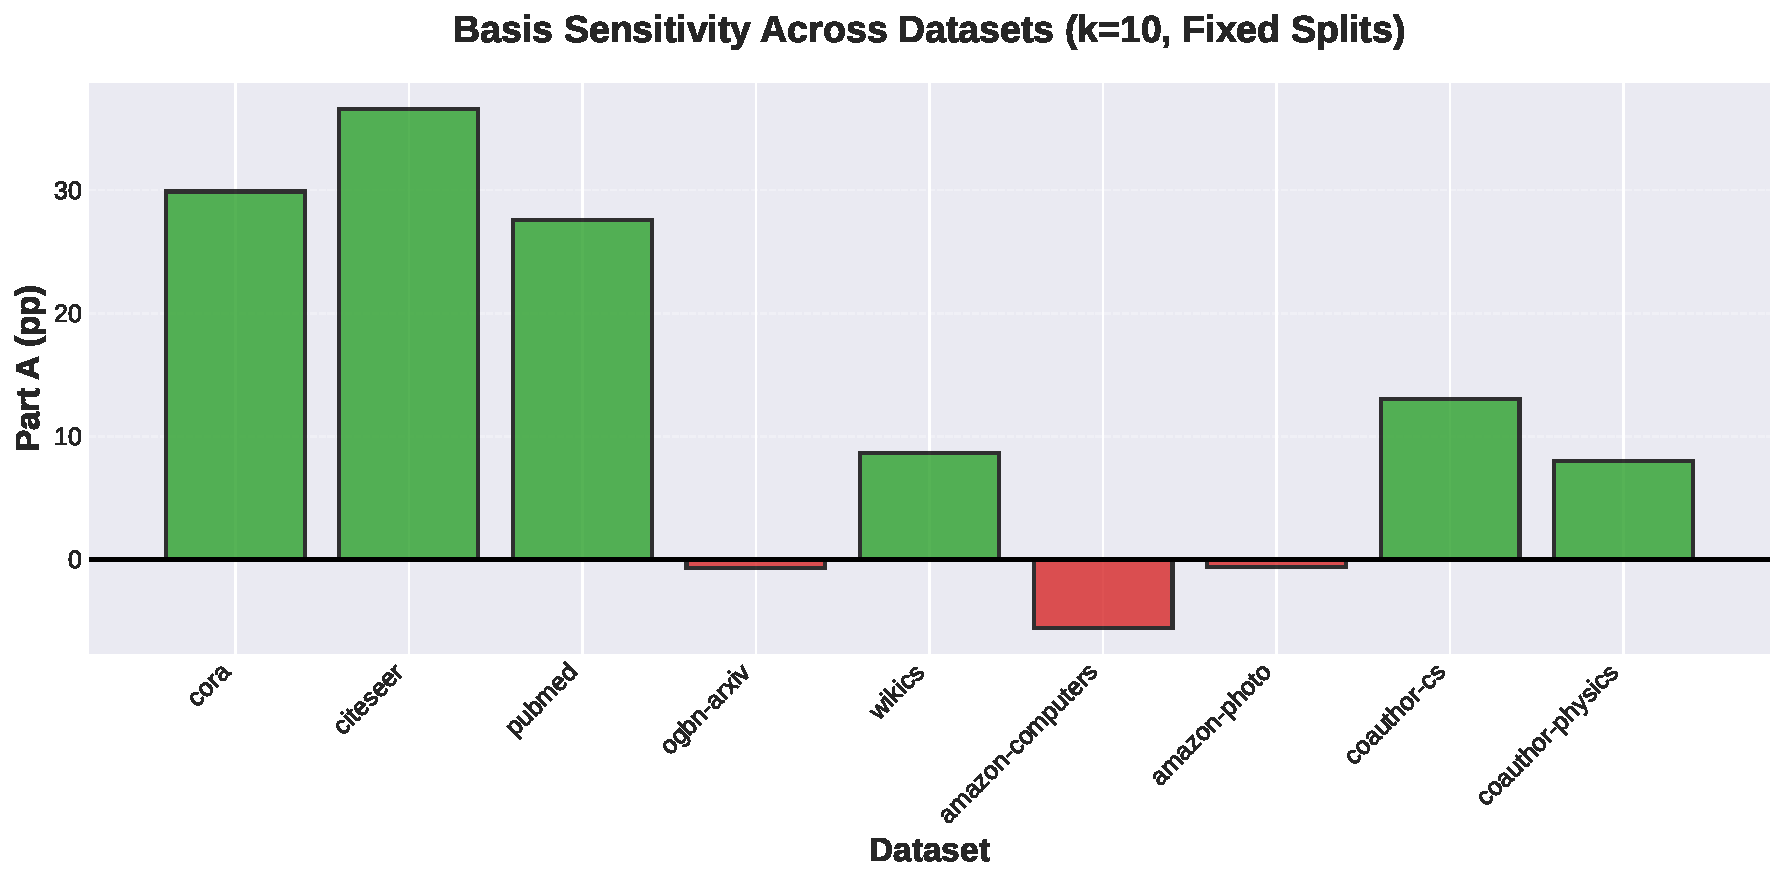
\includegraphics[width=\textwidth]{figures/figure_3_1_part_a_barchart_fixed.pdf}
  \caption{Fixed splits}
\end{subfigure}
\hfill
\begin{subfigure}[b]{0.48\textwidth}
  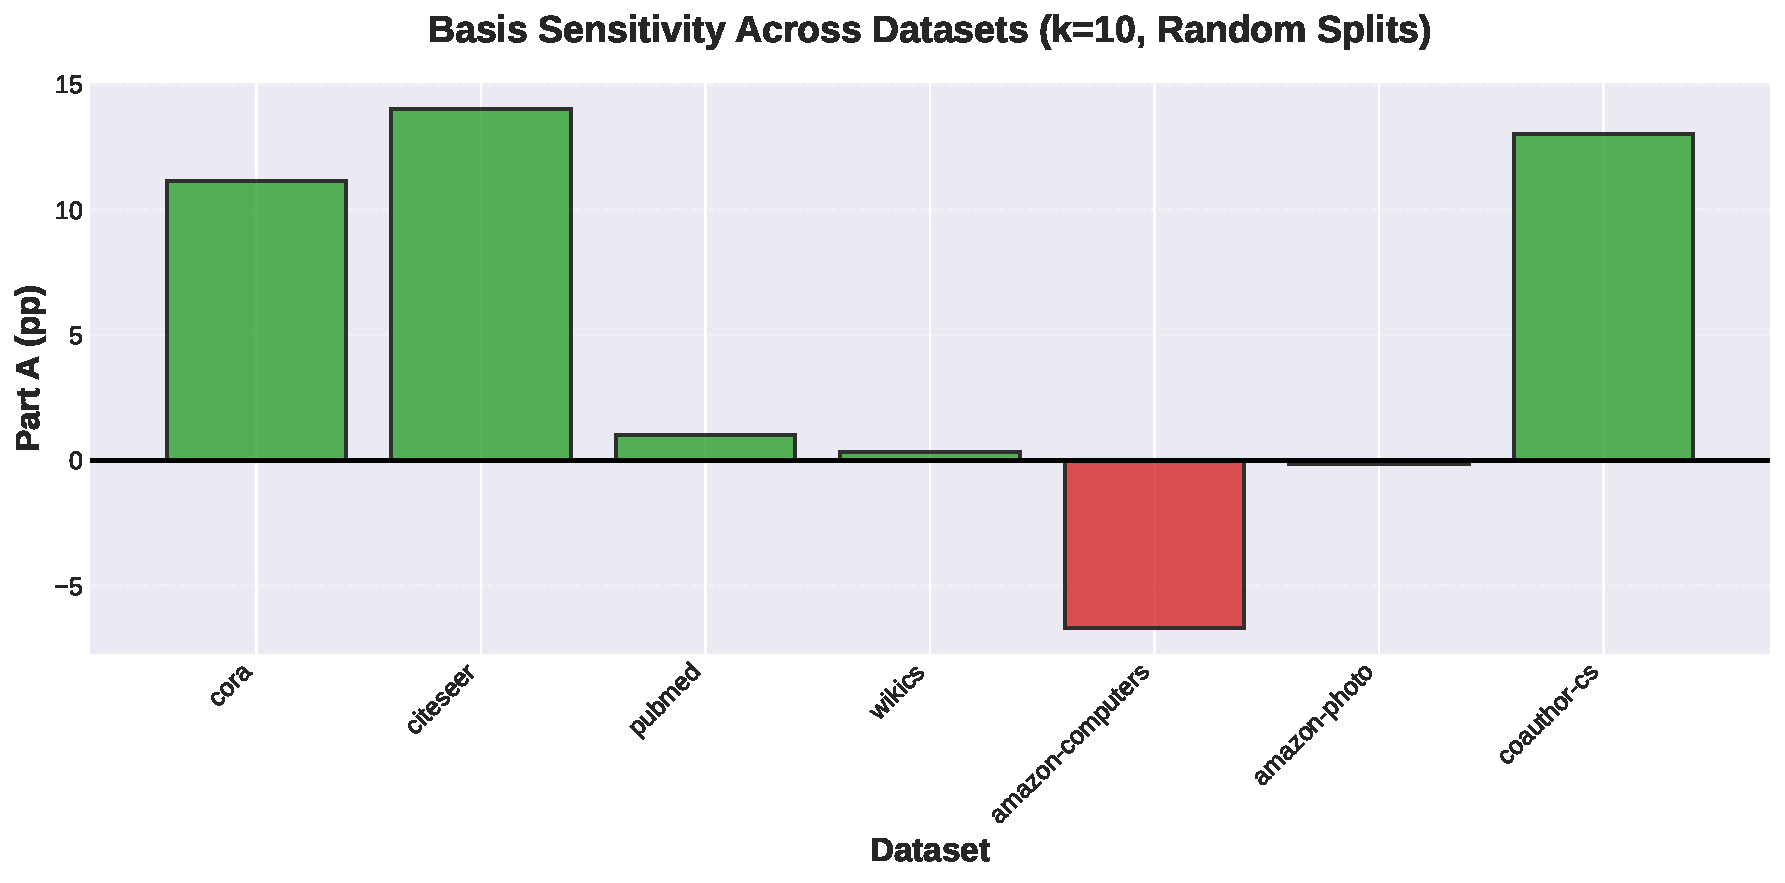
\includegraphics[width=\textwidth]{figures/figure_3_1_part_a_barchart_random.pdf}
  \caption{Random splits}
\end{subfigure}
\caption{Part~A (= SGC+MLP $-$ R+Std accuracy, in pp) at optimal $k^*$ per dataset.
Positive bar $=$ eigenvector basis hurts MLP; negative $=$ eigenvector basis helps.
Fixed splits show larger Part~A for Planetoid datasets (Cora, CiteSeer, PubMed)
due to small fixed training sets (only 20 nodes/class labeled).
\textit{\scriptsize Data: \texttt{results.json} at $k{=}k^*$ per dataset;
same source as Tables~\ref{tab:primary_analysis_fixed}~\&~\ref{tab:primary_analysis_random};
generated by \texttt{generate\_paper\_artifacts\_v2.py}.}}
\label{fig:part_a_barchart}
\end{figure}

\subsection{Part A vs.\ $k$ Curves}

% DATA SOURCE (figure_3_2_part_a_vs_k.pdf):
%   results.json for each dataset/k combination (fixed splits)
%   Part A = sgc_mlp - restricted_std at each k in {1,2,4,6,8,10,12,20,30}
%   Same data as tab:part_a_k_sweep_fixed (Table 5)
%   Generated by: generate_paper_artifacts_v2.py
%   Output: PAPER_OUTPUT/figures/figure_3_2_part_a_vs_k.pdf
\begin{figure}[H]
\centering
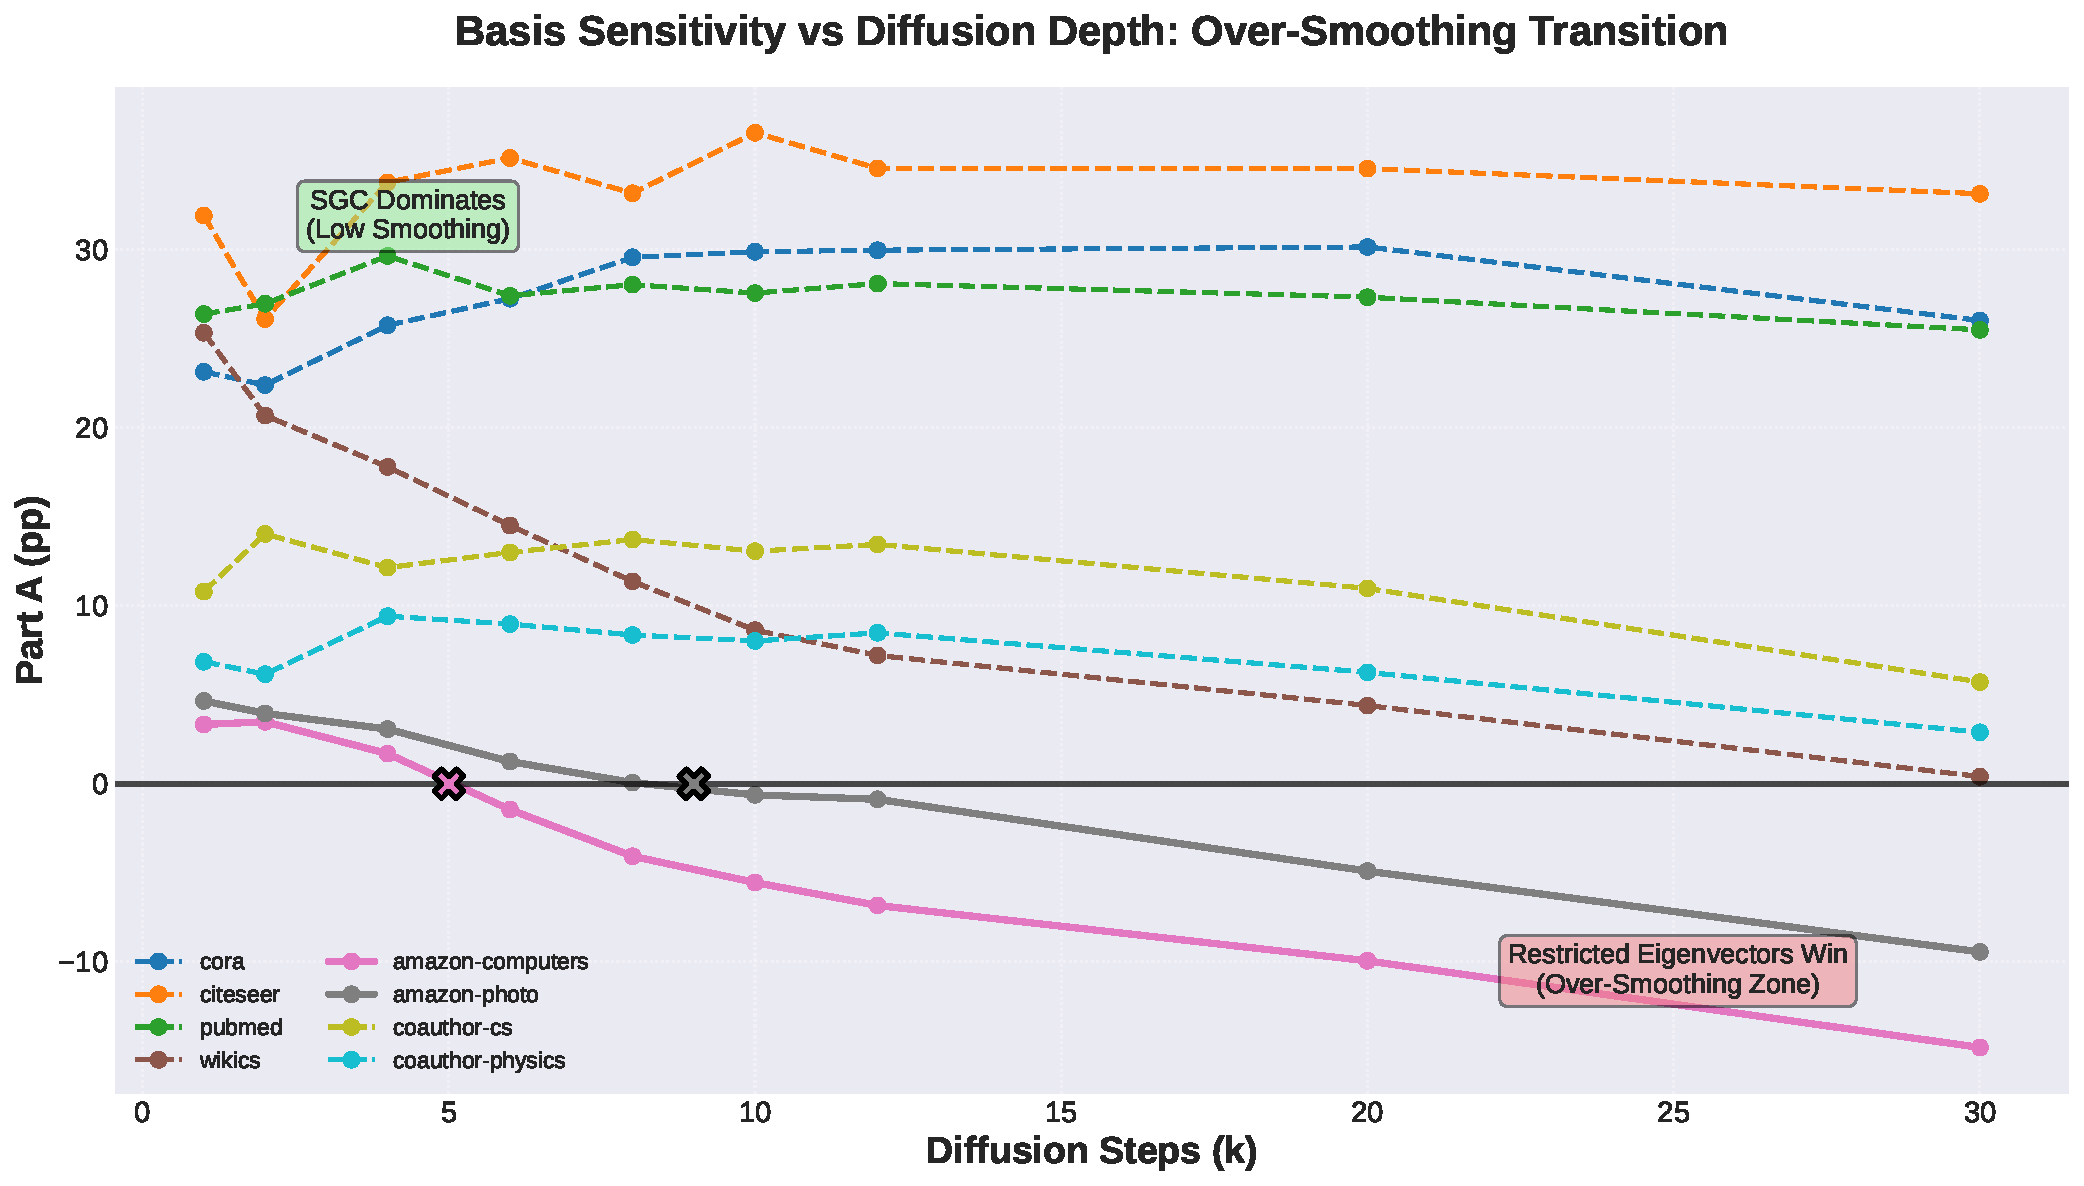
\includegraphics[width=0.95\textwidth]{figures/figure_3_2_part_a_vs_k.pdf}
\caption{Part~A (pp) vs.\ diffusion depth $k$ for all 9 datasets (fixed splits).
Each curve shows how the SGC+MLP $-$ R+Std accuracy gap evolves with $k$.
Four regimes are visible: (1) monotonic positive (citation/collaboration networks---always
above zero), (2) crossover to negative (co-purchase networks---cross zero at $k{\approx}5{-}8$),
(3) deferred crossover (WikiCS---25pp initial gap closes to +0.4pp by $k{=}30$;
crosses at $k{\approx}10{-}12$ under random splits),
(4) weak crossover (ogbn-arxiv---reaches $-3.1$pp at $k{=}30$).
\textit{\scriptsize Data: same as Table~\ref{tab:part_a_k_sweep_fixed};
\texttt{results.json} across all $k$; generated by \texttt{generate\_paper\_artifacts\_v2.py}.}}
\label{fig:part_a_vs_k}
\end{figure}

% DATA SOURCE (figure_3_3_part_b_vs_k.pdf):
%   results.json for each dataset/k combination (fixed splits)
%   Part B = restricted_rownorm - restricted_std at each k
%   Generated by: generate_paper_artifacts_v2.py
%   Output: PAPER_OUTPUT/figures/figure_3_3_part_b_vs_k.pdf
\subsection{Part B vs.\ $k$ Curves}

\begin{figure}[H]
\centering
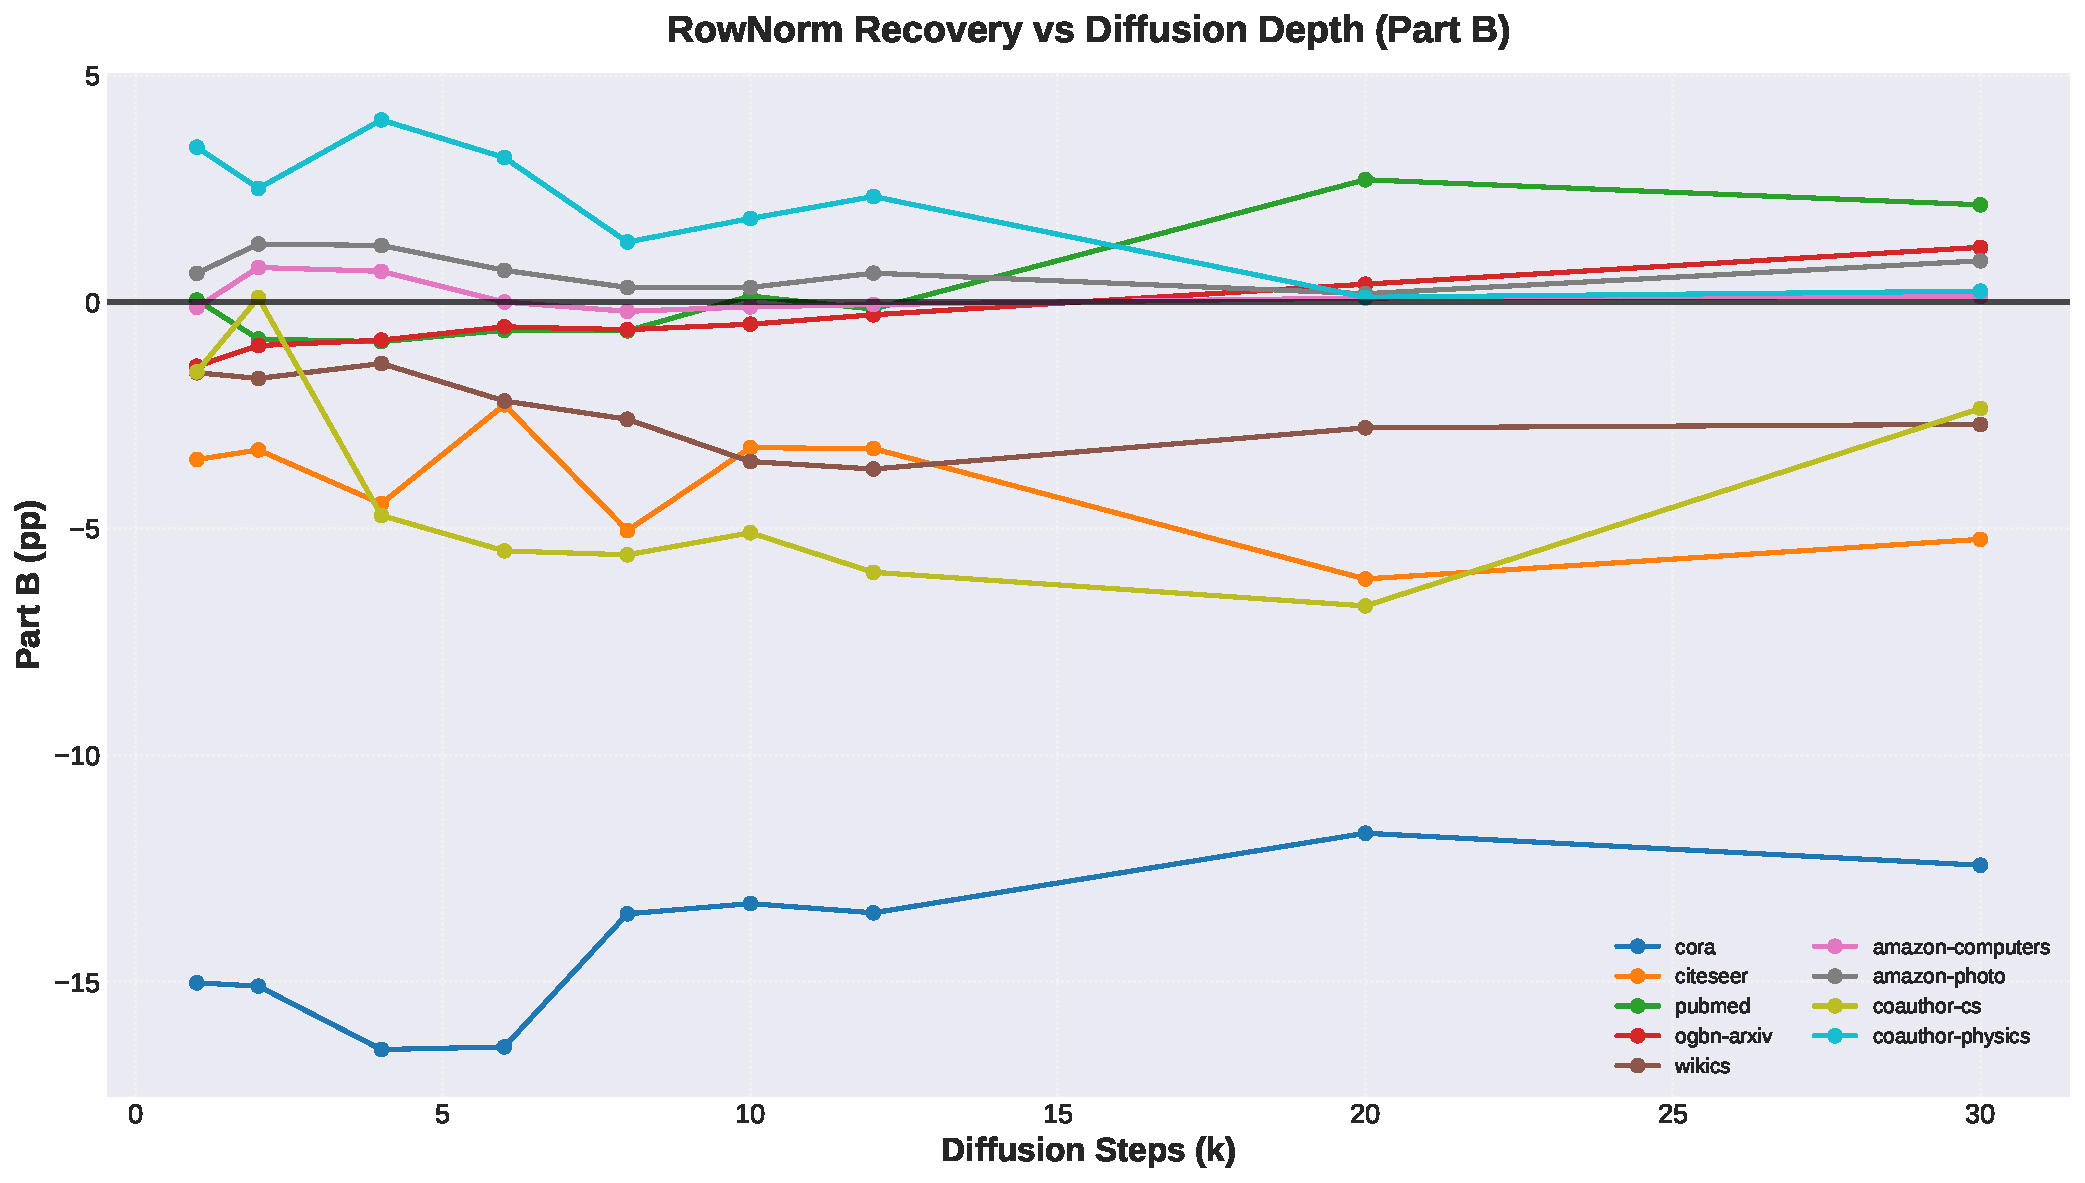
\includegraphics[width=0.95\textwidth]{figures/figure_3_3_part_b_vs_k.pdf}
\caption{Part~B (= R+RN $-$ R+Std accuracy, in pp) vs.\ diffusion depth $k$
for all 9 datasets (fixed splits).
Positive Part~B $=$ RowNorm helps; negative $=$ RowNorm hurts.
Part~B $< 0$ is the \emph{dominant} behavior on monotonic datasets,
showing RowNorm is not a universal remedy for the basis-sensitivity problem.
\textit{\scriptsize Data: \texttt{results.json} fields
\texttt{restricted\_rownorm $-$ restricted\_std} at each $k$;
generated by \texttt{generate\_paper\_artifacts\_v2.py}.}}
\label{fig:part_b_vs_k}
\end{figure}

\subsection{Singular Values}

% DATA SOURCE (figure_4_1_singular_values.pdf):
%   exp2_spectral_analysis_k10.json keys:
%     analysis.singular_values_U_top20  (top 20 SVs of U[train])
%     analysis.singular_values_X_top20  (top 20 SVs of X_diffused[train])
%   Computed by: master_analytics.py:compute_spectral_analysis() lines 111-132
%   Generated by: generate_paper_artifacts_v2.py
%   Output: PAPER_OUTPUT/figures/figure_4_1_singular_values.pdf
\begin{figure}[H]
\centering
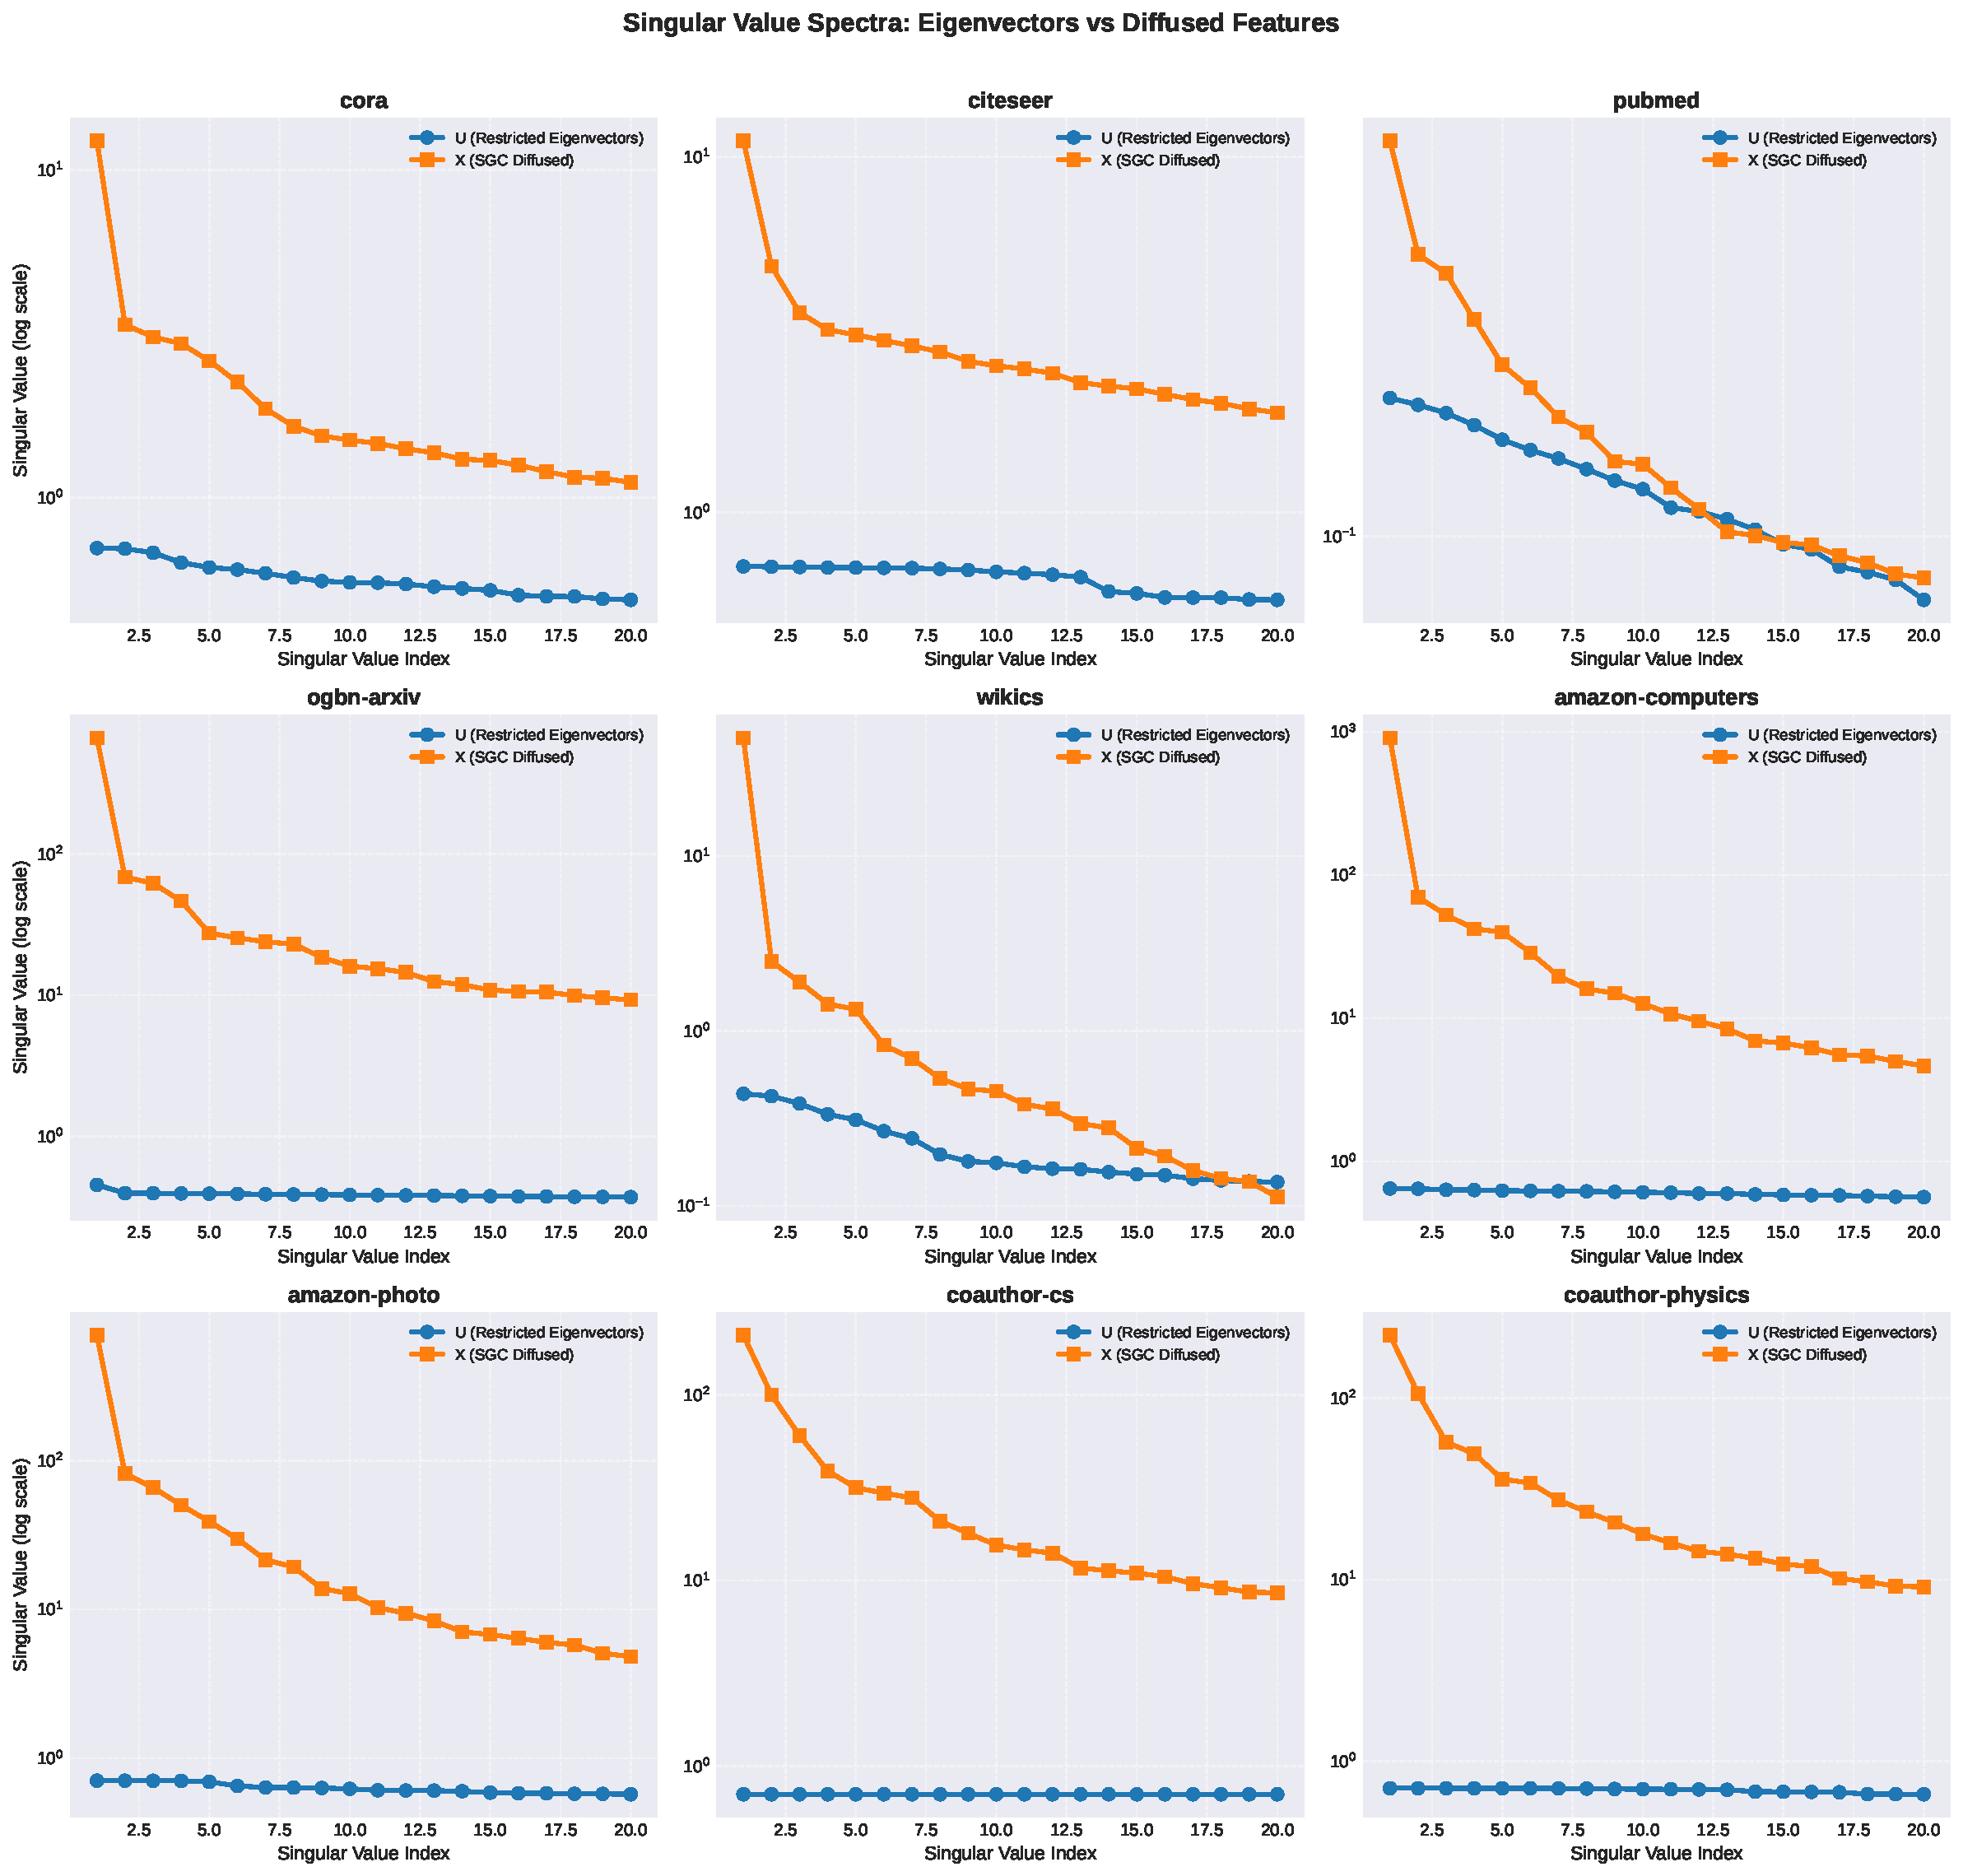
\includegraphics[width=0.95\textwidth]{figures/figure_4_1_singular_values.pdf}
\caption{Singular value spectra of $U$ (restricted eigenvectors) and $X_{\mathrm{diff}}$
($= \hat{A}^k X$) at $k{=}10$, computed on training nodes.
Purpose: show that Rayleigh-Ritz reshapes the singular value distribution---replacing
the power-law decay of $X_{\mathrm{diff}}$ (dominated by a few large directions)
with a more uniform spectrum in $U$ (eigenvectors are spread over the full $d_{\mathrm{eff}}$
dimensions).  This spectral reshaping is the \emph{geometric} explanation of Part~A.
\textit{\scriptsize Data: \texttt{exp2\_spectral\_analysis\_k10.json} keys
\texttt{singular\_values\_U\_top20} and \texttt{singular\_values\_X\_top20};
\texttt{master\_analytics.py:compute\_spectral\_analysis()};
generated by \texttt{generate\_paper\_artifacts\_v2.py}.}}
\label{fig:singular_values}
\end{figure}

\subsection{Alignment vs.\ Spectral Gap}

% DATA SOURCE (figure_4_2_alignment_vs_gap.pdf):
%   X-axis: spectral gap = lambda_2 of Laplacian L (second smallest eigenvalue)
%           from exp2_spectral_analysis_k10.json key eigenvalue_stats.min (lambda_1 ~ 0 for LCC)
%           OR: computed separately as the Fiedler value lambda_2 of L
%   Y-axis: mean_canonical_correlation from exp2_spectral_analysis_k10.json key subspace_alignment
%   Each point = one dataset at k=10
%   Generated by: generate_paper_artifacts_v2.py
%   Output: PAPER_OUTPUT/figures/figure_4_2_alignment_vs_gap.pdf
\begin{figure}[H]
\centering
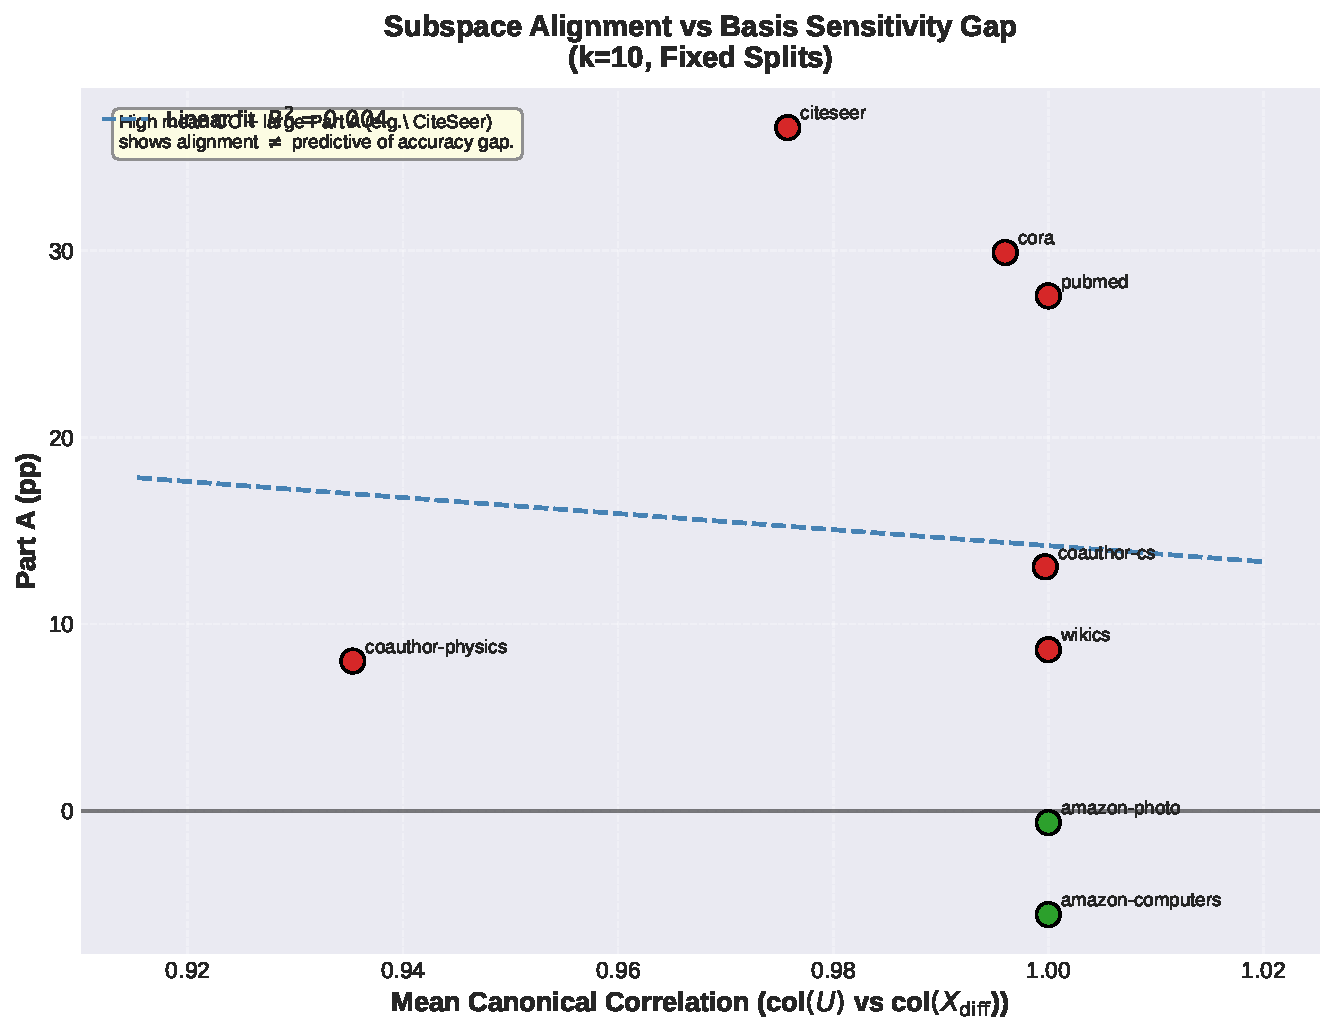
\includegraphics[width=0.75\textwidth]{figures/figure_4_2_alignment_vs_gap.pdf}
\caption{Subspace alignment (Mean CC, see \S\ref{sec:metrics_provenance}) vs.\ spectral
gap $\lambda_2(L)$ (Fiedler value of the graph Laplacian) at $k{=}10$.
Each point is one dataset (fixed split).
Purpose: test whether subspace preservation depends on how well-separated the eigenvalues are.
High alignment ($\mathrm{MeanCC} > 0.93$) regardless of spectral gap confirms
span preservation is not related to eigenvalue separation---the Rayleigh-Ritz
projection is exact even for graphs with small spectral gaps.
\textit{\scriptsize Data: \texttt{exp2\_spectral\_analysis\_k10.json} keys
\texttt{subspace\_alignment.mean\_canonical\_correlation} and \texttt{eigenvalue\_stats};
generated by \texttt{generate\_paper\_artifacts\_v2.py}.}}
\label{fig:alignment_vs_gap}
\end{figure}

% DATA SOURCE (per-dataset training curve figures):
%   PAPER_RESULTS/{dataset}_fixed_lcc/k10/training_curves/split{i}_dynamics.json
%   Same source as figure_6_1_all_training_curves.pdf; one PDF per dataset
%   Generated by: generate_paper_artifacts_v2.py
%   Outputs: PAPER_OUTPUT/figures/figure_6_1_cora_training_curves.pdf
%            PAPER_OUTPUT/figures/figure_6_1_amazon-computers_training_curves.pdf
%            PAPER_OUTPUT/figures/figure_6_1_coauthor-cs_training_curves.pdf
%            PAPER_OUTPUT/figures/figure_6_1_ogbn-arxiv_training_curves.pdf
%   (Plus 5 more datasets; all 9 datasets available as separate PDFs)
\subsection{Training Curves by Dataset}

\begin{figure}[H]
\centering
\begin{subfigure}[b]{0.48\textwidth}
  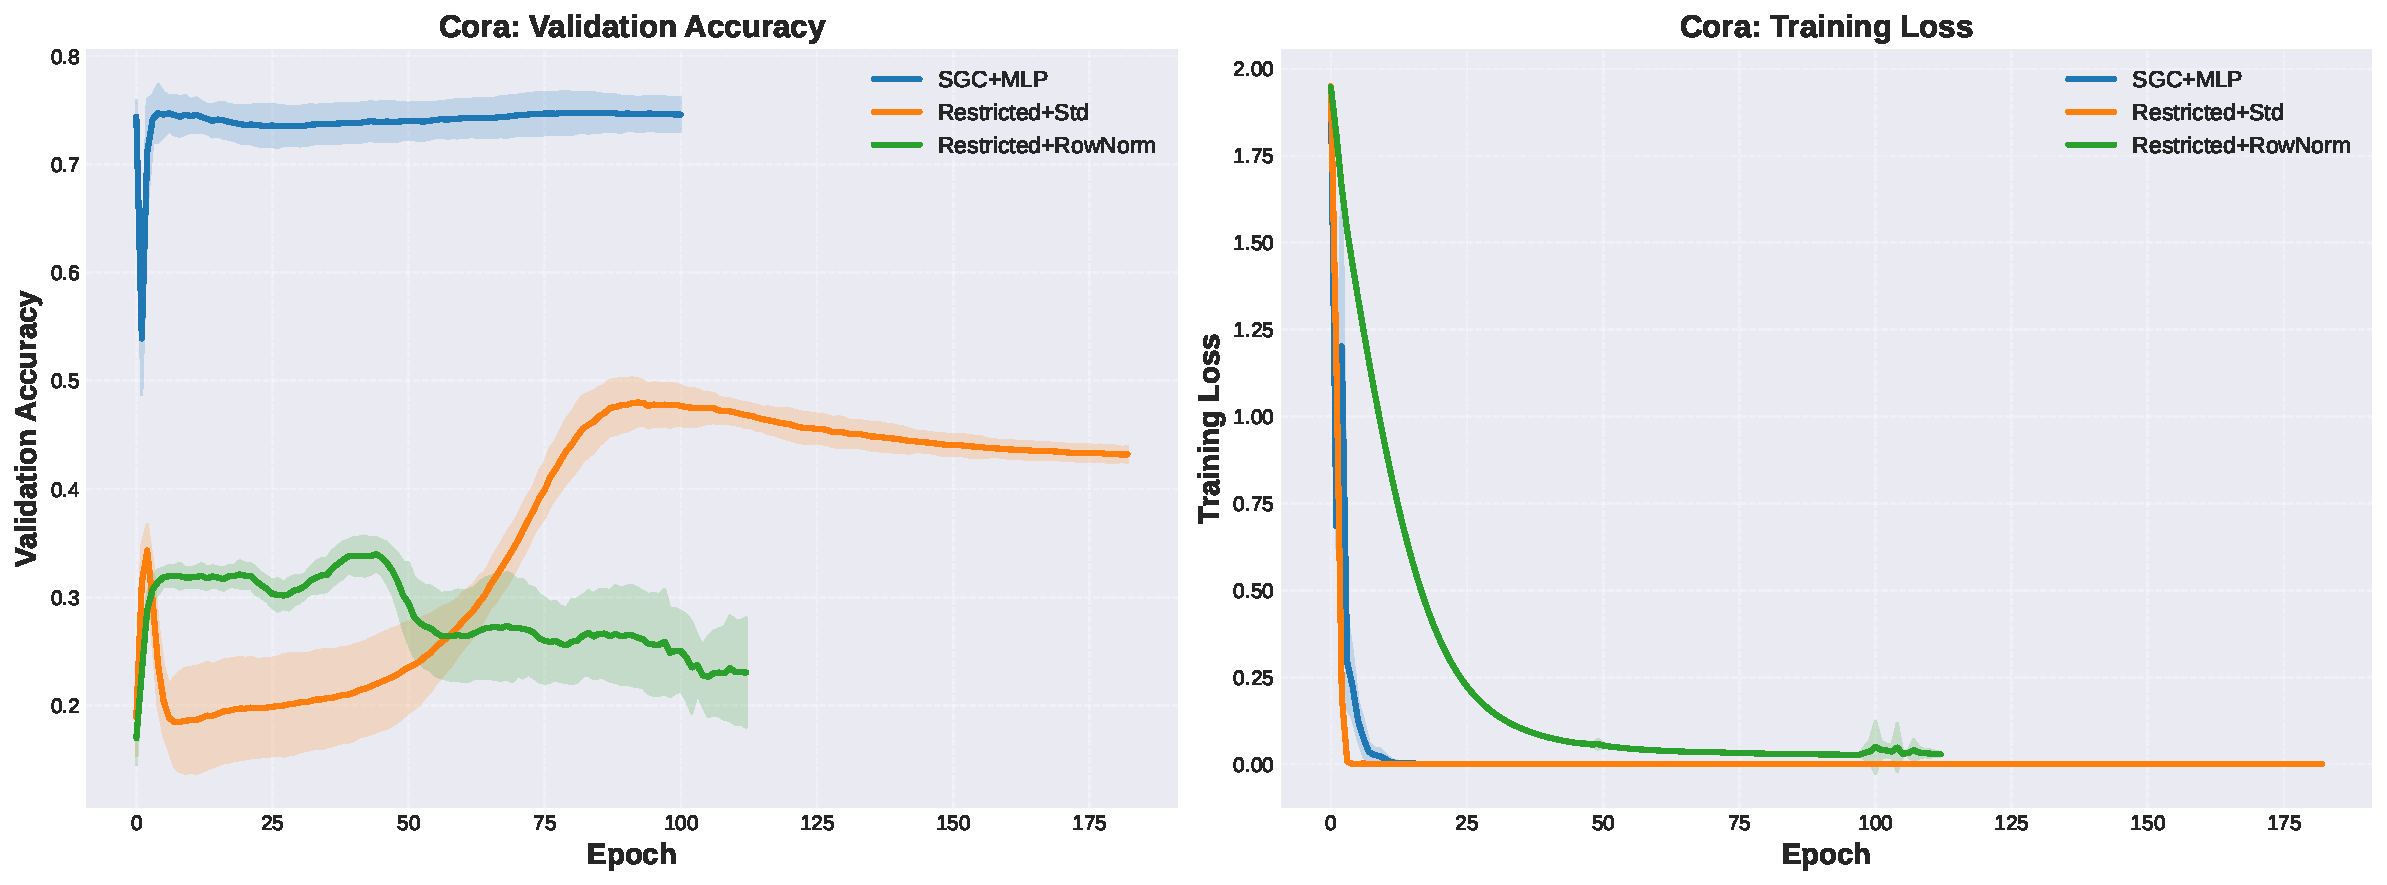
\includegraphics[width=\textwidth]{figures/figure_6_1_cora_training_curves.pdf}
  \caption{Cora (monotonic, large gap; Part~A $= +30$pp)}
\end{subfigure}
\hfill
\begin{subfigure}[b]{0.48\textwidth}
  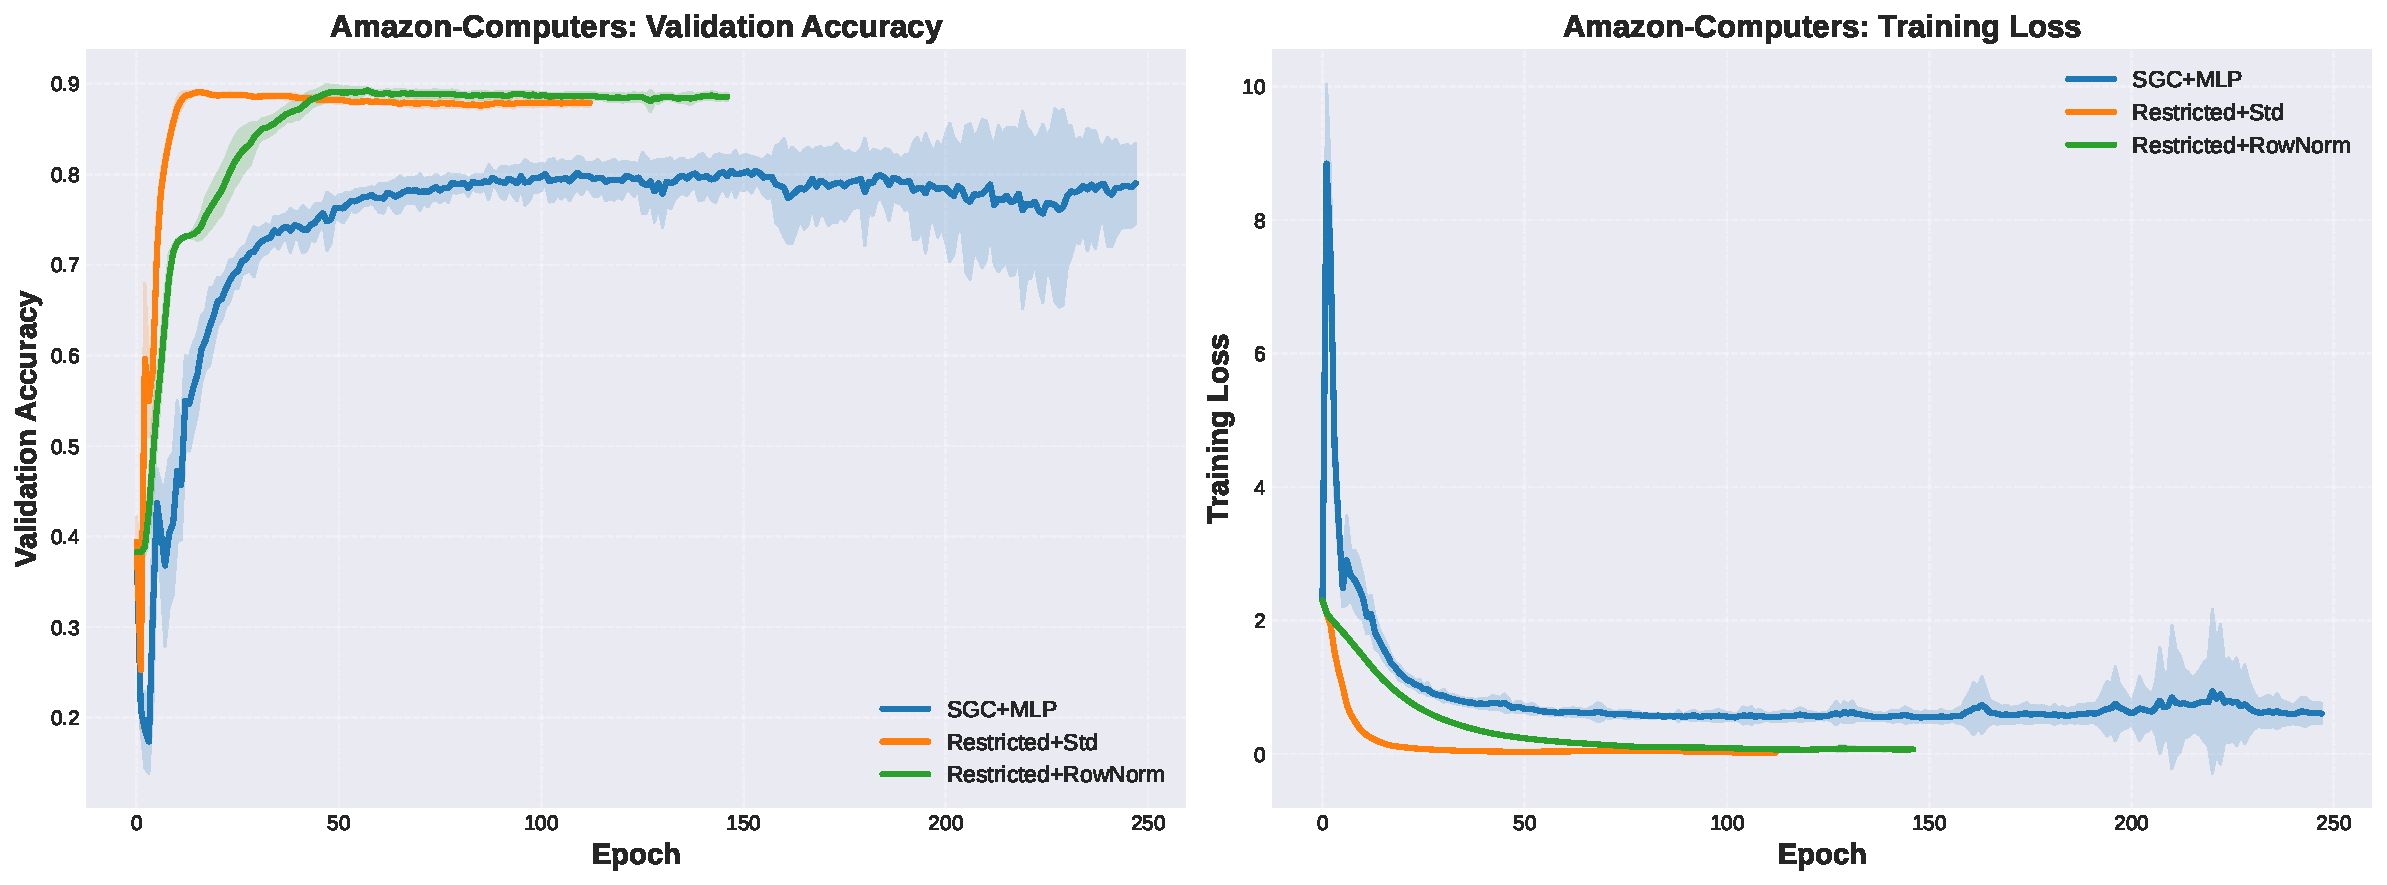
\includegraphics[width=\textwidth]{figures/figure_6_1_amazon-computers_training_curves.pdf}
  \caption{Amazon-Computers (crossover; Part~A $= -5.5$pp at $k{=}10$)}
\end{subfigure}
\\[0.5em]
\begin{subfigure}[b]{0.48\textwidth}
  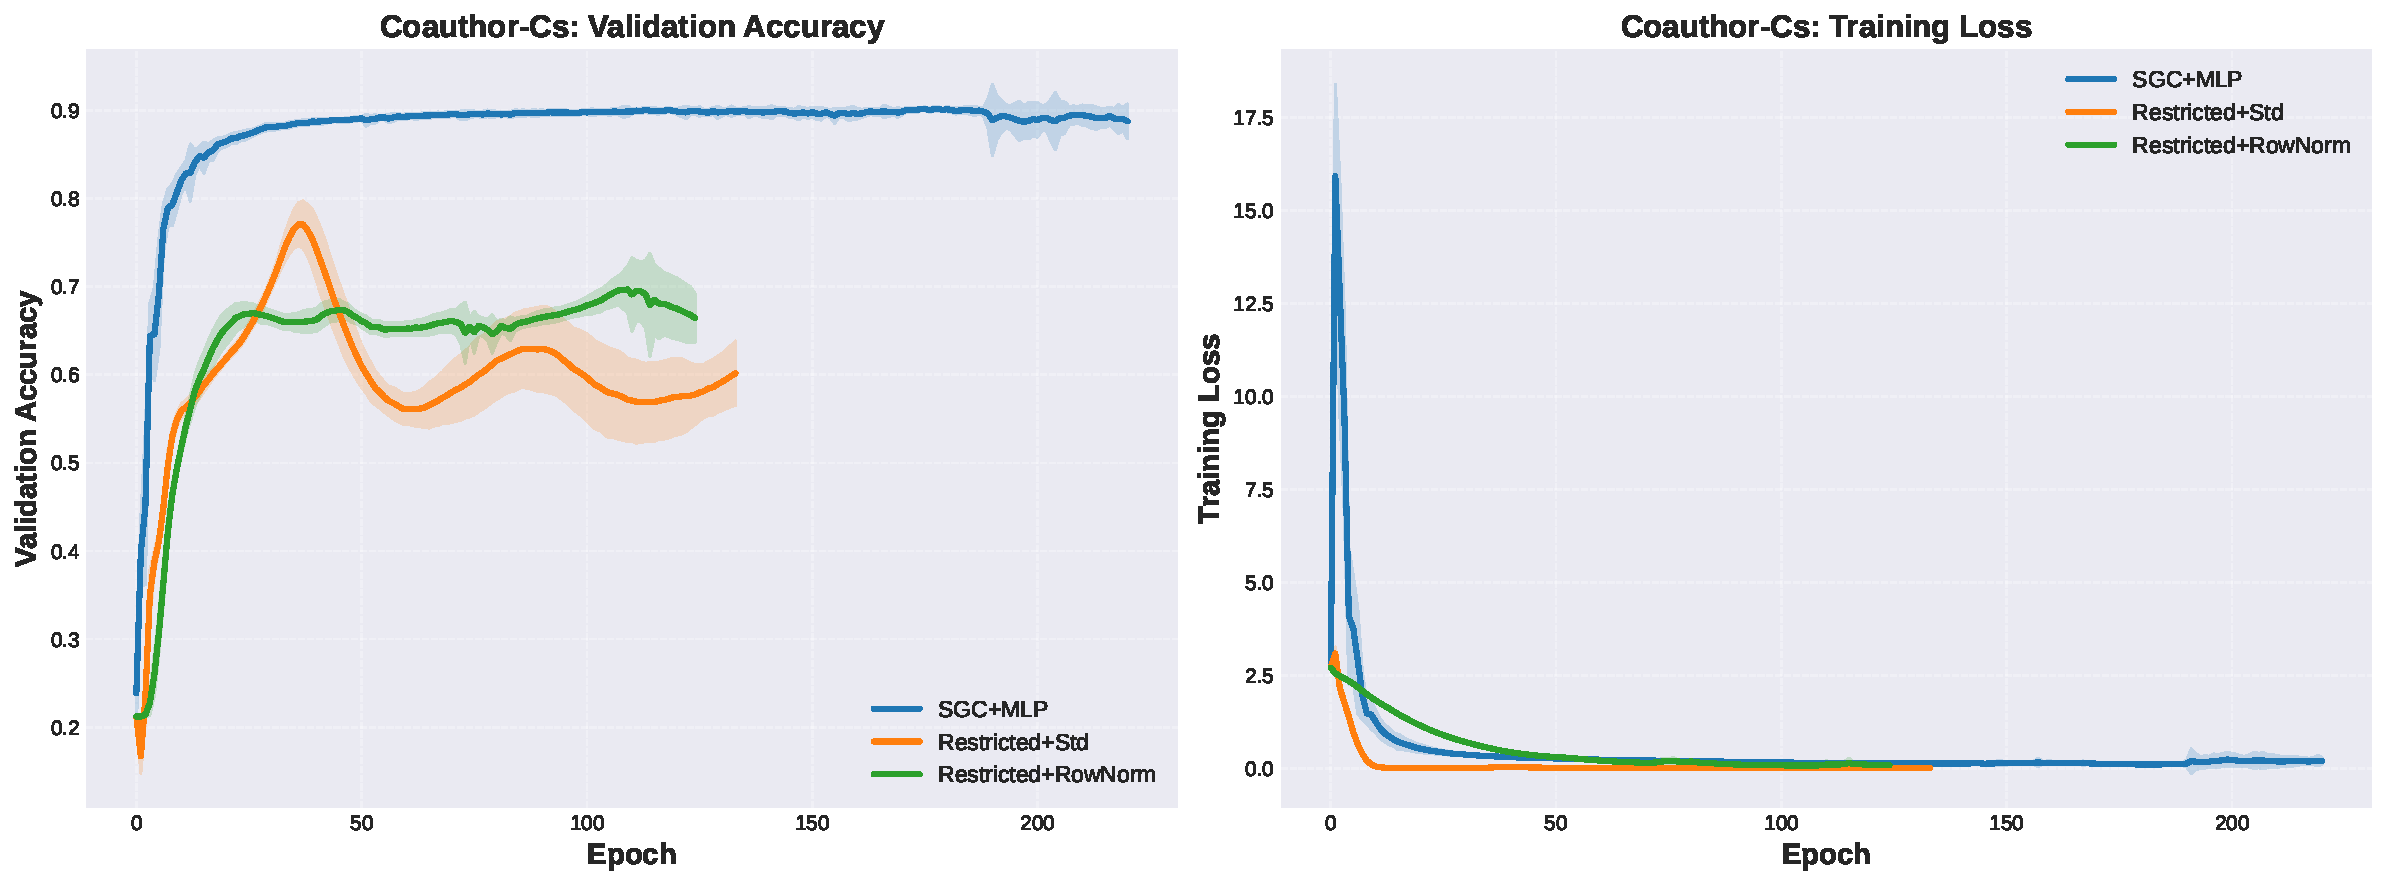
\includegraphics[width=\textwidth]{figures/figure_6_1_coauthor-cs_training_curves.pdf}
  \caption{Coauthor-CS (monotonic; Part~A $= +13$pp)}
\end{subfigure}
\hfill
\begin{subfigure}[b]{0.48\textwidth}
  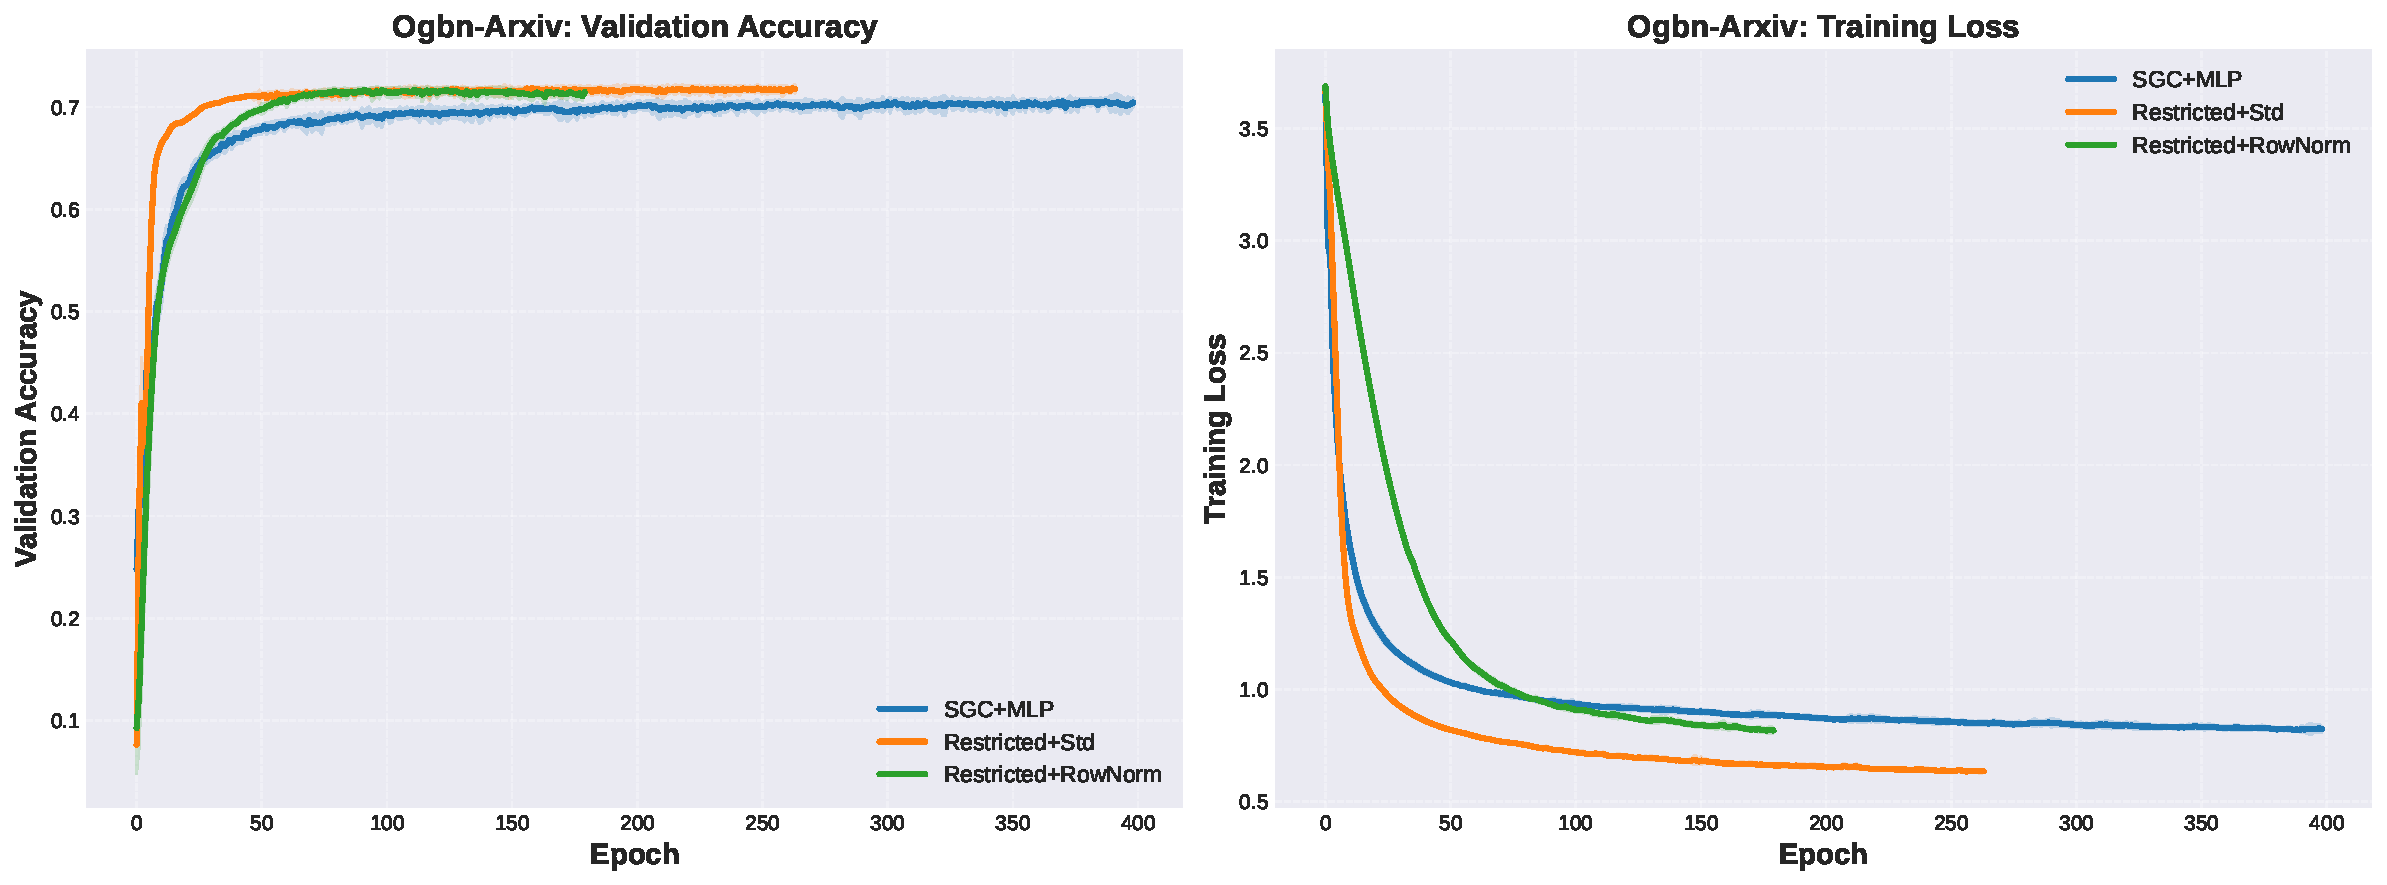
\includegraphics[width=\textwidth]{figures/figure_6_1_ogbn-arxiv_training_curves.pdf}
  \caption{ogbn-arxiv (weak crossover; Part~A $= -0.7$pp at $k{=}10$)}
\end{subfigure}
\caption{Representative training curves (test accuracy vs.\ epoch) at $k{=}10$,
one pair per behavioral regime. Shaded region $=$ 1 std over 15 seeds.
Cora (monotonic): SGC+MLP reaches 90\% of peak in 1 epoch; R+Std requires 82 epochs.
Amazon-Computers (crossover): R+Std converges in 8 epochs vs.\ 40 for SGC+MLP,
and reaches higher final accuracy---the eigenvector basis is \emph{beneficial} here.
\textit{\scriptsize Data: \texttt{training\_curves/split*\_dynamics.json};
\texttt{master\_training.py} Exp~7; generated by \texttt{generate\_paper\_artifacts\_v2.py}.
All 9 datasets available as individual PDFs in \texttt{PAPER\_OUTPUT/figures/}.}}
\label{fig:training_curves_selected}
\end{figure}

% ─────────────────────────────────────────────────────────────────────────────
\section{Synthesis: The Phase Transition Mechanism}
\textit{Question: What single mechanism explains all observed phenomena?}
\label{sec:synthesis}

\subsection{The Unified Mechanism}

The primary empirical findings on monotonic datasets follow from a single structural fact:
\textbf{D-orthonormalization destroys eigenvalue-weighted variance structure}.
The crossover behavior on dense graphs requires an additional mechanism ---
diffusion-induced signal dispersion --- described in \S\ref{sec:phases}.

The Rayleigh-Ritz procedure enforces $U^\top \tilde{D} U = I$,
equalizing \emph{graph-weighted} variance across all eigenvector dimensions.
This does \emph{not} equalize Euclidean variance.
By Proposition~\ref{prop:energy_inversion}(ii), Euclidean column norms are
bounded in $[1/\sqrt{\tilde{d}_{\max}},\, 1/\sqrt{\tilde{d}_{\min}}]$,
independent of eigenvalue rank.
In $X_{\mathrm{diff}} = \hat{A}^k X$, by contrast, each frequency component is
naturally weighted by $(1{-}\lambda_j)^k$, which concentrates energy in the
directions most relevant to the graph's community structure.
Rayleigh-Ritz removes this weighting, inverting the spectral energy hierarchy.

The downstream consequences are:
\begin{enumerate}
  \item \textbf{Representation hardness}: A logistic regression on $U$ is
    27--37pp below SGC+MLP on monotonic datasets, nearly matching the MLP's
    shortfall (MLP vs LR: at most 10pp).  The bulk of the gap is inherent to
    the representation; the MLP recovers at most 10pp over logistic regression,
    leaving the majority unrecovered by nonlinearity alone.
  \item \textbf{Eigenvalue-range dependency}: Datasets with large eigenvalue ranges
    (CiteSeer: 234$\times$; Cora: 76$\times$) incur catastrophic column-variance
    disparity ($10^6$--$10^9$-fold), making high-frequency columns near-constant.
    Small-range datasets (PubMed: 8.9$\times$; dense graphs: all columns at similar
    scale) suffer less.
  \item \textbf{Recoverability}: When class signal is concentrated in low-frequency
    eigenvectors (monotonic datasets), re-amplifying those components via
    $\alpha{=}-1$ partially restores the lost structure and recovers 41--47pp.
    When signal is dispersed (crossover datasets), no monotone reweighting has leverage.
  \item \textbf{The crossover}: On dense graphs, rapid diffusion uniformly spreads
    class signal across all frequency components.  We interpret the crossover in
    Part~A as SGC+MLP degrading through over-smoothing while $U$-space classifiers
    remain comparatively stable (signal is dispersed but present): Part~A crosses
    zero at the point where SGC's over-smoothing loss exceeds the
    D-orthonormalization penalty of $U$.
\end{enumerate}

\subsection{Formal Analysis}

We state two propositions that together explain the root mechanism.
All proofs use only linear algebra and the definition of $\tilde{D}$-orthonormality.
No theorem about the full Laplacian eigenvectors is required; the statements
apply directly to the Rayleigh-Ritz restricted eigenvectors used in all experiments.

\paragraph{Notation.}
Two separate spectral systems appear in the analysis and must be kept distinct.

\textit{Diffusion system.}
$\tilde{A} = A + I$,
$\tilde{D} = \mathrm{diag}(\tilde{d}_1,\ldots,\tilde{d}_n)$ (degree matrix of
$\tilde{A}$), $\hat{A} = \tilde{D}^{-1/2}\tilde{A}\tilde{D}^{-1/2}$ (symmetric
normalized adjacency with self-loops),
$\hat{L} = I - \hat{A} = \tilde{D}^{-1/2}(\tilde{D}-\tilde{A})\tilde{D}^{-1/2}$
(normalized Laplacian with self-loops).
Its eigenvectors $\phi_j$ and eigenvalues $\mu_j$ satisfy
$\hat{L}\phi_j = \mu_j\phi_j$, $\|\phi_j\|_2 = 1$,
$0 \leq \mu_1 \leq \cdots \leq \mu_n < 2$ for connected graphs with self-loops.
These govern the spectral decomposition of $X_{\mathrm{diff}} = \hat{A}^k X_0$.

\textit{Rayleigh-Ritz system.}
$L = D - A$ (unnormalized Laplacian, no self-loops),
$D = \mathrm{diag}(d_1,\ldots,d_n)$ (plain degree matrix, no self-loops).
The restricted eigenvectors are computed as $U = QV$ where
$Q \in \mathbb{R}^{n\times d_{\mathrm{eff}}}$ ($Q^\top Q = I_{d_{\mathrm{eff}}}$)
is the orthonormal basis for $\mathrm{span}(X_{\mathrm{diff}})$, and
$V = [v_1,\ldots,v_{d_{\mathrm{eff}}}]$ solves the projected generalized eigenproblem:
\[
  (Q^\top L Q)\,V \;=\; (Q^\top D Q)\,V\,\Lambda,
  \qquad
  V^\top (Q^\top D Q)\,V = I,
\]
where $\Lambda = \mathrm{diag}(\lambda_1,\ldots,\lambda_{d_{\mathrm{eff}}})$
are the Rayleigh-Ritz eigenvalue approximations (eigenvalues of
$D^{-1/2}LD^{-1/2}$ restricted to $\mathrm{span}(X_{\mathrm{diff}})$).
This yields $U^\top D U = V^\top(Q^\top D Q)V = I$ directly.
The Rayleigh-Ritz property guarantees $\mathrm{span}(U) = \mathrm{span}(X_{\mathrm{diff}})$
(Eq.~\ref{eq:span_invariance}) regardless of which generalized eigenproblem is used
inside the subspace; subspace alignment is verified empirically (Mean CC $> 0.935$,
Table~\ref{tab:subspace_alignment}), confirming that the span invariance holds
numerically to error $< 10^{-9}$ across all 81 dataset-$k$ combinations.

% ── Proposition 1 ──────────────────────────────────────────────────────────────
\begin{proposition}[Spectral Energy Inversion under D-Orthonormalization]
\label{prop:energy_inversion}
\hfill

\noindent\textbf{(i) Energy in $X_{\mathrm{diff}}$ is eigenvalue-weighted.}
Let $\Phi = [\phi_1,\ldots,\phi_n]$ be the orthonormal eigenvectors of $\hat{L}$
($\hat{L}\phi_j = \mu_j\phi_j$, $\|\phi_j\|_2 = 1$).
The diffused features $X_{\mathrm{diff}} = \hat{A}^k X_0$ decompose as:
\[
  X_{\mathrm{diff}} \;=\; \sum_{j=1}^{n} (1-\mu_j)^k\,\phi_j\,(\phi_j^\top X_0).
\]
The Frobenius energy in the $j$-th eigendirection is
$(1{-}\mu_j)^{2k}\|\phi_j^\top X_0\|_F^2$,
weighted by $|1-\mu_j|^{2k}$: this weight decreases on $[0,1]$, increases on $[1,2]$,
and is minimized at $\mu_j = 1$.
In the homophilous non-bipartite graphs used in this work ($\mu_n < 2$),
class-discriminative signal is predominantly low-frequency ($\mu_j \approx 0$),
so diffusion acts as an effective low-pass filter in practice.

\noindent\textbf{(ii) Euclidean column norms of $U$ are eigenvalue-independent.}
For each column $u_j$ of the $D$-orthonormal matrix $U = QV$:
\[
  \frac{1}{\sqrt{d_{\max}}} \;\leq\; \|u_j\|_2 \;\leq\; \frac{1}{\sqrt{d_{\min}}}
\]
where $d_{\min} = \min_i d_i$ and $d_{\max} = \max_i d_i$ (plain degrees, no self-loops).
This bound is \emph{independent of $\lambda_j$}.

\noindent\textbf{Consequence.}
$D$-orthonormalization abolishes the diffusion-induced basis-vector norm hierarchy of
$X_{\mathrm{diff}}$.
In $X_{\mathrm{diff}}$, the ratio of energy between two eigendirections $p$ and $q$ is:
\[
  \frac{\|\Pi_p X_{\mathrm{diff}}\|_F^2}{\|\Pi_q X_{\mathrm{diff}}\|_F^2}
  \;=\;
  \frac{|1-\mu_p|^{2k}}{|1-\mu_q|^{2k}}
  \cdot
  \frac{\|\Pi_p X_0\|_F^2}{\|\Pi_q X_0\|_F^2}.
\]
In particular, when $\mu_p \approx 0$ (low-frequency) and $\mu_q \approx 1$
(mid-spectrum), the first factor grows as $(1-\mu_p)^{2k} \gg |1-\mu_q|^{2k}$,
amplifying any initial energy imbalance exponentially with $k$
(whenever the initial spectral energies $\|\Pi_p X_0\|_F^2$,
$\|\Pi_q X_0\|_F^2$ are comparable).

In $U$, the ratio of Euclidean column norms is bounded by $\sqrt{d_{\max}/d_{\min}}$
regardless of $k$ or $\lambda_j$, by part~(ii).
\end{proposition}

\begin{proof}
\textbf{Part (i).}
Since $\hat{A} = \Phi(I-\mathrm{M})\Phi^\top$ where $\mathrm{M} = \mathrm{diag}(\mu_1,\ldots,\mu_n)$,
and $\Phi^\top\Phi = I$:
\[
  X_{\mathrm{diff}} = \hat{A}^k X_0
  = \Phi(I-\mathrm{M})^k\Phi^\top X_0
  = \sum_{j=1}^n (1-\mu_j)^k\,\phi_j\,(\phi_j^\top X_0).
\]
Since the $\phi_j$ are orthonormal, the terms are orthogonal in $\mathbb{R}^n$.
The Frobenius norm of the $j$-th term is
$\|(1-\mu_j)^k\phi_j(\phi_j^\top X_0)\|_F^2
= (1-\mu_j)^{2k}\|\phi_j^\top X_0\|_F^2$
(using $\|\phi_j\|_2 = 1$).
The weight $|1-\mu_j|^{2k}$ is
monotonically decreasing on $[0,1]$ and increasing on $[1,2]$; it is minimized at
$\mu_j = 1$ and maximized at the endpoints $\mu_j \in \{0,2\}$.
In the non-bipartite graphs used in this work ($\mu_n < 2$), the dominant
low-pass behavior holds: components with $\mu_j \approx 0$ retain the most energy.

\textbf{Part (ii).}
Write $u_j = Qv_j$ where $Q^\top Q = I_{d_{\mathrm{eff}}}$.
Then $\|u_j\|_2^2 = v_j^\top Q^\top Q v_j = \|v_j\|_2^2$.
The $D$-orthonormality condition gives
$u_j^\top D u_j = v_j^\top(Q^\top D Q)v_j = 1$.
Let $M = Q^\top D Q \in \mathbb{R}^{d_{\mathrm{eff}}\times d_{\mathrm{eff}}}$.
Since $d_{\min}I \preceq D \preceq d_{\max}I$:
\[
  d_{\min}\,\|v_j\|_2^2 \;\leq\; v_j^\top M v_j \;=\; 1
  \;\leq\; d_{\max}\,\|v_j\|_2^2.
\]
Rearranging gives $1/d_{\max} \leq \|v_j\|_2^2 \leq 1/d_{\min}$,
and therefore $1/d_{\max} \leq \|u_j\|_2^2 \leq 1/d_{\min}$.
Taking square roots gives the stated bound.
The bound involves only $d_{\min}$ and $d_{\max}$; it does not
involve $\lambda_j$.  \qed
\end{proof}

\begin{remark}[On the empirically observed large variance ratios]
\label{rem:variance_ratios}
Proposition~\ref{prop:energy_inversion}(ii) bounds column \emph{norms}, not column
\emph{variances}.
The large empirical variance ratios in Table~\ref{tab:eigenvalue_range} (up to
$2{\times}10^9$ for CiteSeer) arise because some columns of $U$ are approximately
constant: their mean $\bar{u}_j \approx \|u_j\|_2/\sqrt{n}$, making their variance
$\|u_j\|_2^2/n - \bar{u}_j^2 \approx 0$.
This near-constancy is topology-dependent.
For the lowest-frequency eigenvector ($\lambda_1 \approx 0$), the normalized Laplacian
eigenvector of the RR system satisfies
$\phi_1^{(RR)} \approx D^{1/2}\mathbf{1}/\|D^{1/2}\mathbf{1}\|_2$
(the Fiedler-limit Perron vector of the random walk), giving
$u_1 = D^{-1/2}\phi_1^{(RR)} \approx \mathbf{1}/\|D^{1/2}\mathbf{1}\|_2$
--- a near-constant vector with variance $\approx 0$.
More generally, on the homophilous graphs considered here, several low-frequency
modes are empirically smoother and more degree-aligned, so their transformed
coordinates $u_j = D^{-1/2}\phi_j^{(RR)}$ can exhibit low Euclidean variance.
This is an empirical observation on these benchmark graphs, not a general theorem.
The correlation between eigenvalue range and empirical variance ratio is therefore
real but operates through degree-eigenvector alignment, not through an algebraic
$1/\lambda_j^2$ identity.
\end{remark}

% ── Proposition 2 ──────────────────────────────────────────────────────────────
\begin{proposition}[Near-Constant Columns Receive Near-Zero Discriminative Gradient Signal]
\label{prop:gradient_collapse}
Let logistic regression with weight matrix $W \in \mathbb{R}^{C\times d_{\mathrm{eff}}}$
and bias $b \in \mathbb{R}^C$ be trained on features $U \in \mathbb{R}^{n\times d_{\mathrm{eff}}}$
with cross-entropy loss.
The gradient of $\mathcal{L}$ with respect to $W_{c,j}$ (weight connecting feature $j$
to class $c$) decomposes as:
\[
  \frac{\partial \mathcal{L}}{\partial W_{c,j}}
  \;=\;
  \underbrace{-\bar{u}_j \sum_i (y_{ic} - p_{ic})}_{\text{bias-equivalent (non-discriminative)}}
  \;\;-\;\;
  \underbrace{\sum_i (y_{ic} - p_{ic})(u_j(i) - \bar{u}_j)}_{\text{discriminative signal}}
\]
where $p_{ic} = \mathrm{softmax}(Wu_i + b)_c$, $y_{ic} \in \{0,1\}$, and
$\bar{u}_j = n^{-1}\sum_i u_j(i)$.
The discriminative component satisfies:
\[
  \left|\sum_i (y_{ic} - p_{ic})(u_j(i) - \bar{u}_j)\right|
  \;\leq\; n \cdot \mathrm{Std}(U_{:,j})
\]
where $\mathrm{Std}(U_{:,j}) = \sqrt{\mathrm{Var}(U_{:,j})}$.
As $\mathrm{Var}(U_{:,j}) \to 0$, the discriminative gradient signal from feature $j$
vanishes regardless of the model weights.
\end{proposition}

\begin{proof}
The gradient of cross-entropy w.r.t.\ $W_{c,j}$ is:
\[
  \frac{\partial \mathcal{L}}{\partial W_{c,j}} = -\sum_i (y_{ic} - p_{ic})\,u_j(i).
\]
Write $u_j(i) = \bar{u}_j + (u_j(i) - \bar{u}_j)$ and separate:
\[
  = -\bar{u}_j\sum_i(y_{ic} - p_{ic}) - \sum_i(y_{ic} - p_{ic})(u_j(i) - \bar{u}_j).
\]
The first term $-\bar{u}_j\sum_i(y_{ic} - p_{ic})$ equals $\bar{u}_j$ times the
gradient w.r.t.\ the bias $b_c$.
It encodes only mean-level class imbalance, not inter-class discriminative variation
from feature $j$ beyond what the bias already captures.
At any stationary point (in particular the optimum), $\partial\mathcal{L}/\partial b_c
= -\sum_i(y_{ic}-p_{ic}) = 0$, so this term vanishes.

For the discriminative component, by the triangle inequality:
\[
  \left|\sum_i(y_{ic} - p_{ic})(u_j(i)-\bar{u}_j)\right|
  \;\leq\; \max_i|y_{ic}-p_{ic}| \cdot \sum_i|u_j(i)-\bar{u}_j|.
\]
Since $y_{ic} \in \{0,1\}$ and $p_{ic} \in (0,1)$, we have $\max_i|y_{ic}-p_{ic}| \leq 1$.
By Cauchy-Schwarz, $\sum_i|u_j(i)-\bar{u}_j| \leq \sqrt{n}\,\|u_j - \bar{u}_j\mathbf{1}\|_2
= \sqrt{n}\cdot\sqrt{n\cdot\mathrm{Var}(U_{:,j})} = n\cdot\mathrm{Std}(U_{:,j})$.
Therefore:
\[
  \left|\sum_i(y_{ic}-p_{ic})(u_j(i)-\bar{u}_j)\right| \;\leq\; n\cdot\mathrm{Std}(U_{:,j}).
\]
As $\mathrm{Var}(U_{:,j}) \to 0$ (column $j$ becomes constant),
$\mathrm{Std}(U_{:,j}) \to 0$ and the bound goes to zero. \qed
\end{proof}

\begin{remark}[Extension to MLPs and Adam]
\label{rem:mlp_adam}
Proposition~\ref{prop:gradient_collapse} is stated for logistic regression because
the gradient decomposition is exact in the linear case.
For an $L$-layer MLP, the first-layer weight gradient is
$\partial\mathcal{L}/\partial W^{(1)}_{:,j} = \sum_i \delta_i\,u_j(i)$ where
$\delta_i \in \mathbb{R}^h$ is the backpropagated signal to the first hidden layer.
The bias-equivalent/discriminative decomposition carries through with
$\delta_i$ in place of $(y_{ic}-p_{ic})$; the bound becomes
$\|\partial\mathcal{L}/\partial W^{(1)}_{:,j}\|_2 \leq \mathrm{Std}(U_{:,j})\cdot C_\theta$
where $C_\theta = n\max_i\|\delta_i\|_2$ depends on the remaining weights.
The LR experimental evidence (Table~\ref{tab:lr_vs_sgc}: MLP vs LR $\leq$ 10pp
on all datasets) confirms that the same mechanism operates in the nonlinear setting
--- a deeper model cannot recover gradient signal that is absent due to near-constant
columns.

For \textbf{Adam}: the effective update for weight $W_{c,j}$ is
$\hat{g}_j/(\sqrt{\hat{v}_j} + \epsilon_{\mathrm{Adam}})$ where $\hat{g}_j,\hat{v}_j$
are bias-corrected first and second gradient moments.
When column $j$ is $\epsilon$-constant, $|\hat{g}_j| = O(\epsilon)$ and
$\hat{v}_j = O(\epsilon^2)$ by the proposition.
The adaptive step is $O(\epsilon)/(\sqrt{O(\epsilon^2)} + \epsilon_{\mathrm{Adam}})
= O(1)$ only when $\sqrt{\hat{v}_j} \ll \epsilon_{\mathrm{Adam}} = 10^{-8}$,
i.e., only when $\hat{v}_j \ll 10^{-16}$ --- a regime not reached in practice.
Adam therefore provides only marginal rescue for near-constant columns; both
numerator and denominator grow proportionally with $\epsilon$, leaving the
effective signal-to-noise ratio unchanged.
\end{remark}

% ── Proposition 3 ──────────────────────────────────────────────────────────────
\begin{proposition}[Row Normalization Cannot Increase Bayes-Optimal Accuracy]
\label{prop:rownorm_bound}

Let $U \in \mathbb{R}^{n \times d}$ be a feature matrix for a $C$-class node
classification problem with labels $y \in \{1,\ldots,C\}$.
Define the row-normalized representation
\[
  \tilde{U}_i \;=\; \frac{U_i}{\|U_i\|_2}, \qquad i = 1,\ldots,n.
\]
Then:
\begin{enumerate}[label=(\roman*)]
  \item \textbf{Information bound.}
    The Bayes-optimal accuracy satisfies
    \[
      \mathrm{Acc}^*(\tilde{U}) \;\leq\; \mathrm{Acc}^*(U).
    \]
    Row normalization cannot increase the achievable accuracy ceiling.

  \item \textbf{Equality condition.}
    A sufficient condition for equality is that the row magnitude $\|U_i\|_2$
    carries no additional class information beyond what the direction $\tilde{U}_i$
    already provides:
    \[
      \|U_i\|_2 \;\perp\; y_i \;\mid\; \tilde{U}_i.
    \]
    In particular, this holds when $\mathrm{Fisher}(U) = 0$
    (all class-conditional magnitude distributions are identical).

  \item \textbf{Diagnostic interpretation of Part~B.}
    When $\mathrm{Part~B} > 0$ empirically --- meaning an MLP on $\tilde{U}$
    outperforms an MLP on $U$ --- this does not contradict~(i).
    It implies that the MLP on $U$ is \emph{optimization-limited}:
    \[
      \mathrm{Acc}_{\mathrm{MLP}}(U) \;<\; \mathrm{Acc}^*(U),
    \]
    and RowNorm improves optimization (better-conditioned loss landscape, reduced
    column-variance disparity) enough to offset the information loss.
    Part~B $> 0$ therefore diagnoses optimization failure, not representation
    improvement.
\end{enumerate}
\end{proposition}

\begin{proof}
\textbf{Part~(i).}
The map $\psi: U_i \mapsto U_i/\|U_i\|_2$ is a deterministic function of $U_i$.
By the \textbf{data processing inequality} for Shannon mutual information,
for any deterministic function $\psi$:
\[
  I(\tilde{U}_i;\, y_i) \;=\; I(\psi(U_i);\, y_i) \;\leq\; I(U_i;\, y_i).
\]
Since Bayes-optimal accuracy is a non-decreasing function of mutual information
(more precisely, $\mathrm{Acc}^*(X) \leq 1 - H(y|X)/\log C$ and
$H(y|X)$ is non-increasing in $I(X;y)$), we conclude
\[
  \mathrm{Acc}^*(\tilde{U}) \;\leq\; \mathrm{Acc}^*(U).
\]

\textbf{Alternatively, via posterior averaging.}
For any class $c$, the tower property of conditional expectation gives:
\[
  P(y_i = c \mid \tilde{U}_i)
  \;=\; \mathbb{E}\bigl[P(y_i = c \mid U_i) \;\big|\; \tilde{U}_i\bigr].
\]
This holds because $\tilde{U}_i = \psi(U_i)$ is a coarsening of $U_i$:
any event measurable w.r.t.\ $\tilde{U}_i$ is measurable w.r.t.\ $U_i$.
Now apply Jensen's inequality to the convex function $\max_c(\cdot)$:
\[
  \max_c P(y_i = c \mid \tilde{U}_i)
  \;=\; \max_c \mathbb{E}\bigl[P(y_i=c\mid U_i)\;\big|\;\tilde{U}_i\bigr]
  \;\leq\; \mathbb{E}\bigl[\max_c P(y_i=c\mid U_i)\;\big|\;\tilde{U}_i\bigr].
\]
Taking expectations over $\tilde{U}_i$ and applying the law of total expectation:
\[
  \mathrm{Acc}^*(\tilde{U})
  = \mathbb{E}\Bigl[\max_c P(y_i=c\mid\tilde{U}_i)\Bigr]
  \leq \mathbb{E}\Bigl[\max_c P(y_i=c\mid U_i)\Bigr]
  = \mathrm{Acc}^*(U). \quad \checkmark
\]

\textbf{Part~(ii).}
Equality in Jensen holds if and only if $\max_c P(y_i=c\mid U_i)$ is
$\sigma(\tilde{U}_i)$-measurable, i.e., the optimal class assignment is the
same for all $U_i$ sharing the same direction.
This requires the argmax posterior to be constant on each ray
$\{rU_i : r > 0\}$, which is equivalent to $\|U_i\|_2$ providing no
additional discriminative information:
$\|U_i\|_2 \perp y_i \mid \tilde{U}_i$.

When $\mathrm{Fisher}(U) = 0$, the between-class variance of magnitudes is zero,
meaning $\mathbb{E}[\|U_i\|_2 \mid y_i = c]$ is the same for all $c$.
Under any symmetric noise model, this implies
$P(\|U_i\|_2 \mid y_i, \tilde{U}_i) = P(\|U_i\|_2 \mid \tilde{U}_i)$,
i.e., magnitude is class-conditionally independent of label given direction.

\textbf{Part~(iii).}
Suppose $\mathrm{Acc}_{\mathrm{MLP}}(\tilde{U}) > \mathrm{Acc}_{\mathrm{MLP}}(U)$.
By part~(i), $\mathrm{Acc}^*(\tilde{U}) \leq \mathrm{Acc}^*(U)$.
Therefore:
\[
  \mathrm{Acc}_{\mathrm{MLP}}(U)
  < \mathrm{Acc}_{\mathrm{MLP}}(\tilde{U})
  \leq \mathrm{Acc}^*(\tilde{U})
  \leq \mathrm{Acc}^*(U).
\]
The MLP on $U$ is strictly below its own Bayes ceiling.
The gap $\mathrm{Acc}^*(U) - \mathrm{Acc}_{\mathrm{MLP}}(U)$ is the
\emph{optimization gap} on $U$.
RowNorm reduces this gap by improving the optimization landscape
(Proposition~\ref{prop:gradient_collapse}: reducing column-variance
disparity increases discriminative gradient signal).
The net effect on accuracy is positive when the optimization gain
exceeds the information loss. \qed
\end{proof}

\begin{remark}[Why Part~B is negative on most datasets]
\label{rem:partb_negative}
Proposition~\ref{prop:rownorm_bound}(i) bounds the \emph{ceiling}, not the
\emph{achieved} accuracy.
When $\mathrm{Fisher}(U) > 0$, magnitude carries genuine class signal.
Discarding it via RowNorm both loses this signal (ceiling decreases) and improves
optimization (gap to ceiling shrinks).
Part~B is negative when the signal loss dominates; positive when the optimization
gain dominates.
The empirical pattern --- Part~B $< 0$ on 7/9 datasets at their optimal $k^*$,
with the exceptions being datasets where Fisher scores remain moderate
(Amazon-Photo, Coauthor-Physics) --- is exactly consistent with this analysis:
magnitude carries recoverable class signal on those datasets, and the optimization
gain from RowNorm does not compensate.
\end{remark}

\subsection{Three Phases of Diffusion}
\label{sec:phases}

The phase transition is most precisely understood as a competition between two effects
of the Rayleigh-Ritz projection operating simultaneously at every $k$:

\begin{description}
  \item[Effect 1 — Beneficial noise filtering:]
    The restricted eigenvector computation projects $X_{\mathrm{diff}}$ onto the
    Laplacian eigenvector basis, retaining only directions that are smooth on the graph.
    High-frequency feature components inconsistent with community structure are removed.
    This filtering helps any downstream classifier.
  \item[Effect 2 — Harmful variance destruction:]
    D-orthonormalization equalizes graph-weighted variance across all eigenvector
    dimensions, destroying the eigenvalue-weighted column-variance ordering that
    concentrates signal in class-relevant directions.
    This hurts any downstream classifier in proportion to the eigenvalue range.
\end{description}

Part~A is the net outcome of this competition.  Its sign and magnitude evolve with
$k$ because diffusion changes how much each effect contributes.

\textbf{Phase 1: Universal Benefit ($k = 1{-}2$).}
At shallow diffusion depth, Effect~1 dominates.  $X_{\mathrm{diff}}$ at $k{=}1$ is
only lightly smoothed and still contains substantial high-frequency noise.
The Rayleigh-Ritz step removes this noise before the MLP sees the features, providing
a benefit that diffusion alone has not yet delivered.  Effect~2 is present but mild:
the eigenvalue range of the restricted problem is relatively small at $k{=}1$, so
variance destruction is limited.  All 9/9 datasets show positive Part~A (range:
$+1.1$ to $+31.9$pp, Table~\ref{tab:part_a_k1_stds}).

\textbf{Phase 2: Divergence ($k = 2{-}8$).}
As diffusion depth increases, Effect~1 diminishes — diffusion itself progressively
smooths $X_{\mathrm{diff}}$, reducing the marginal filtering benefit of Rayleigh-Ritz.
Simultaneously, Effect~2 grows as the eigenvalue range of the restricted problem widens.
The rate of this transition depends on graph density:

\emph{Dense graphs (avg degree 20--40):} Rapid diffusion over highly connected networks
causes Effect~1 to vanish within 2--4 steps.
We use the Fisher score of $\|U_i\|$ (dropping 95--99\% within these steps,
Table~\ref{tab:fisher_collapse}) as a diagnostic proxy: when Fisher(U) collapses,
the first Laplacian eigenvector of $U$ carries no class-discriminative signal,
indicating the Laplacian basis is no longer aligned with class structure and the
high-frequency components that Rayleigh-Ritz removes are no longer class-irrelevant noise.
Class signal disperses uniformly across all frequency components, and no filtering
benefit remains.  Effect~2 also grows quickly.  Part~A crosses zero at $k \approx 5{-}8$.

\emph{Sparse graphs (avg degree 3--6):} Slow diffusion within tight communities means
Effect~1 persists: $X_{\mathrm{diff}}$ remains partially noisy at moderate $k$, and
Rayleigh-Ritz continues to provide filtering value.  Effect~2 grows slowly because
sparse graph Laplacians have smaller eigenvalue ranges.  Part~A remains strongly
positive ($+25$--$+37$pp).

\textbf{Phase 3: Stabilization ($k > 10$).}
On crossover datasets, Effect~1 has fully vanished and Part~A reflects only the
D-orthonormalization penalty, continuing to degrade (reaching $-15$pp at $k{=}30$)
as SGC itself degrades through over-smoothing while $U$-space classifiers remain
stable.  On monotonic datasets, Effect~1 has mostly disappeared but Effect~2 also
plateaus because the eigenvalue range stabilizes; Part~A remains positive but
decays slowly at extreme $k$ as rank collapse reduces the available eigenvectors.

\subsection{Why Conditioning Is Not the Mechanism}

WikiCS ($\kappa(U) = 2738$, Part~A~$=+0.4$pp) vs.\ Amazon-Computers ($\kappa(U) = 39$,
Part~A~$=-14.8$pp) at $k{=}30$ demonstrates that numerical conditioning is decoupled
from Part~A behavior by a factor of $\sim70\times$.  Poor conditioning would predict
WikiCS to fail, but it maintains positive Part~A.
The high $\kappa(U)$ for WikiCS is itself explained by spectral collapse of
$X_{\mathrm{diff}}$: the ratio $\sigma_1(X_{\mathrm{diff}})/\sigma_2(X_{\mathrm{diff}})$
grows from 7.3 at $k{=}1$ to 120 at $k{=}30$, forcing the Rayleigh-Ritz to produce
ill-conditioned eigenvectors.  Amazon-Computers, with 767 features and slower spectral
concentration ($\sigma_1/\sigma_2 \leq 22$), keeps $\kappa(U)$ below 66 throughout.
Thus the conditioning contrast is a downstream effect of feature-space dimensionality
and spectral concentration rate, not an independent factor.

\subsection{Why Homophily Is Not the Primary Factor}

Homophily shows only a $4.4\%$ difference between crossover and monotonic datasets
(0.753 vs.\ 0.787).  Amazon-Photo has homophily $= 0.827$ (similar to Cora $= 0.804$)
yet crosses over.  Homophily is not a sufficient predictor of the phase transition;
graph density and diffusion speed are the primary drivers.

\subsection{The $\alpha = -1$ Recovery Insight}

The universal optimality of $\alpha{=}-1$ is not coincidental:
\[
U_{\text{scaled}} = \mathrm{diag}(\lambda_1^{-1}, \ldots, \lambda_{d}^{-1}) \cdot U
\]
Inverse eigenvalue scaling amplifies the low-frequency Laplacian eigenvectors
(small $\lambda_j$, class-aligned signals) and suppresses the high-frequency ones
(large $\lambda_j$, within-class variation).  It partially re-introduces
\emph{a} low-frequency-amplifying weighting, analogous in effect to the
diffusion weighting that D-orthonormalization destroyed, though operating in
the $\lambda_j$ system rather than the $\mu_j$ system of the diffusion operator.

This is \emph{not} equivalent to recovering $X_{\mathrm{diff}}$ geometrically.
Reconstructing $X_{\mathrm{diff}}$ from $U$ would require weighting by $\lambda_j^k$,
not $\lambda_j^{-1}$.  What $\alpha{=}-1$ restores is the \emph{column-variance
ordering}: after scaling, low-frequency columns (high class-relevance on sparse graphs)
are again the dominant directions, as they are in $X_{\mathrm{diff}}$.

\noindent\textbf{Controlled evidence from the $\beta$ ablation.}
The NestedSpheres experiment varies both $\alpha$ (eigenvalue weighting) and $\beta$
(magnitude scalar) independently.  Within any fixed $\alpha$, accuracy varies
only ${\sim}6$pp across all $\beta$ values.  The 47pp recovery on Cora is driven
entirely by $\alpha$; $\beta{=}0$ is optimal.  This rules out a magnitude-based
explanation: the recovery operates through frequency reweighting, not through
exploiting the discriminative information in $\|U_i\|$.

\noindent\textbf{Why recovery fails on crossover datasets.}
The $\alpha$ sweep is flat ($<1$pp range) for Amazon-Computers and ogbn-arxiv
(Table~\ref{tab:alpha_sweep_full_fixed}).  This is the structural flatness of
dispersed signal: when class information is uniform across all frequency buckets,
amplifying any subset of eigenvectors by any monotone function of $\lambda$ cannot
improve separation.  The failure of $\alpha{=}-1$ on crossover datasets and the
positive $\Delta$ in the linear probe (Table~\ref{tab:linear_probe}) are two
measurements of the same underlying fact.

% ─────────────────────────────────────────────────────────────────────────────
\section{Conclusions}
\label{sec:conclusions}

\subsection{Primary Findings}

\begin{enumerate}
  \item \textbf{Universal low-$k$ benefit}: Restricted eigenvectors improve MLP
    performance at $k{=}1$ on \emph{all} 9/9 datasets (range $+1.1$ to $+31.9$pp;
    all ${\geq}2.7\times$ propagated std, Table~\ref{tab:part_a_k1_stds}).
    Static degradation hypotheses are falsified; the relationship is $k$-dependent.

  \item \textbf{Part~A is a representation problem, not optimization}: A logistic
    regression classifier on $U$ matches the 3-layer MLP at most 10pp above a linear classifier on all
    9 datasets (Table~\ref{tab:lr_vs_sgc}).  The MLP's nonlinearity adds almost
    nothing beyond a linear model in $U$-space.  The gap relative to SGC originates
    in the representation itself.

  \item \textbf{Eigenvalue range predicts representation difficulty}: By
    Proposition~\ref{prop:energy_inversion}, D-orthonormalization abolishes the
    eigenvalue-weighted energy hierarchy of $X_{\mathrm{diff}}$; Euclidean column
    norms are bounded by degree statistics, not eigenvalue rank.
    On irregular graphs this produces topology-dependent Euclidean column-variance
    disparity that correlates empirically with eigenvalue range:
    CiteSeer's $234\times$ range produces a $2{\times}10^9$-fold disparity;
    PubMed's $8.9\times$ range produces only $171\times$.
    This predicts the ordering of LR accuracy gaps from SGC and the shape of
    the $p$-vs-accuracy curves in Table~\ref{tab:linear_probe}.

  \item \textbf{Graph density drives crossover, with qualifications}: Dense graphs
    (avg degree ${\sim}30$) exhibit rapid Fisher score collapse ($95$--$99\%$ within
    2--4 steps) and crossover to negative Part~A.  Sparse graphs (avg degree ${\sim}5$)
    maintain concentrated class signal.  However, density alone is not sufficient:
    WikiCS (avg degree $38$, similar to Amazon-Computers $36.7$) does not cross over
    under fixed splits because its large initial gap ($+25.3$pp at $k{=}1$) and
    moderate eigenvalue range ($14.1\times$) interact to defer the crossing.  The
    correct joint predictors of crossover timing are density, initial gap size, and
    spectral concentration rate of $X_{\mathrm{diff}}$.

  \item \textbf{Signal concentration vs.\ dispersion}: Monotonic datasets concentrate
    class information in the first ${\sim}50$ eigenvectors (using more hurts by 25--32pp).
    Crossover datasets disperse signal requiring all $d_{\text{eff}}$ dimensions.
    The concentration/dispersion label predicts both MLP behavior and $\alpha$ leverage.

  \item \textbf{Fisher score as leading indicator}: On dense co-purchase networks,
    Fisher($v_1$) collapse \emph{precedes} Part~A crossover by 1.3--6.2 diffusion steps,
    providing a predictive diagnostic.  On ogbn-arxiv, Fisher remains above threshold
    after Part~A crosses zero, indicating signal disperses across multiple eigenvectors
    rather than collapsing in a single direction.

  \item \textbf{Subspace preservation confirmed}: Mean CC $> 0.935$ and D-orthonormality
    error $< 10^{-9}$ prove the Rayleigh-Ritz projection is mathematically exact.
    Variance structure destruction, not information loss, explains Part~A.

  \item \textbf{Spectral recovery}: Inverse eigenvalue scaling ($\alpha{=}-1$) recovers
    41--47pp on monotonic datasets by reintroducing frequency weighting that
    D-orthonormalization removed.  The $\beta$ magnitude ablation (NestedSpheres) confirms
    that recovery operates through frequency reweighting, not magnitude information.
    Recovery is not universal because crossover datasets have dispersed signal across
    all frequency components, making any monotone reweighting ineffective ($<1$pp range).

  \item \textbf{RowNorm is not universal}: RowNorm hurts on 7/9 datasets at their
    respective $k^*$ (fixed splits), showing Part~B $< 0$ is the norm, not the exception.
    It should not be used as a default remedy.
\end{enumerate}

\subsection{Split-Dependent Anomalies}

\begin{itemize}
  \item CiteSeer Part~B changes sign between fixed ($-5.24$pp) and random ($+4.75$pp),
    indicating that RowNorm's effectiveness depends critically on training set size.
  \item WikiCS and PubMed show crossovers only under random splits, not fixed.
    Larger training coverage reduces the advantage of the spectral basis at high $k$.
\end{itemize}

\subsection{Open Questions}

\textbf{1.\ Theoretical Fisher collapse bounds:} Can we prove that dense graphs
(avg degree $> \theta$) must disperse Fisher score within $O(k)$ diffusion steps?

\textbf{2.\ Why is $U$-space harder for any classifier?}
The logistic regression comparison (Table~\ref{tab:lr_vs_sgc}) establishes that
the difficulty is in the representation, not the optimizer.  The open question is
not why MLPs fail to learn from dispersed signal, but why D-orthonormalization
produces a space that is inherently harder to separate for \emph{any} linear or
nonlinear classifier.  The eigenvalue range explanation (Table~\ref{tab:eigenvalue_range})
addresses the monotonic dataset case, but does not fully explain the crossover
datasets where signal is dispersed rather than obscured by variance collapse.
A complete theory would characterize the classifier hardness of $U$-space
as a function of the graph's spectral properties and the feature-class alignment.

\textbf{3.\ Adaptive diffusion:} Can we design density-aware diffusion schemes that
stop before the crossover point, identified via online Fisher score monitoring?

\textbf{4.\ Generalization to other GNNs:} Do ChebNet, GPRGNN, spectral attention
mechanisms exhibit similar $k$-dependent phase transitions?

\textbf{5.\ Beyond $k{=}30$:} Do monotonic datasets eventually crossover at very
high diffusion, or does community structure permanently protect them?

% ══════════════════════════════════════════════════════════════════════════════
\section{Related Work}
\label{sec:related}
% ══════════════════════════════════════════════════════════════════════════════

\paragraph{Graph diffusion and spectral representations.}
Simple Graph Convolution (SGC)~\citep{wu2019simplifying} showed that the
nonlinearity in GCN~\citep{kipf2017semi} is not essential for competitive
node classification: collapsing the $k$-layer GCN into a single linear map
on $k$-diffused features $X_{\mathrm{diff}} = \hat{A}^k X$ suffices, and in
many settings outperforms deeper models.
This decoupling of diffusion from classification is the starting point of our
investigation.
We construct the Rayleigh-Ritz restricted eigenvector basis $U$ satisfying
\[
  \mathrm{span}(U) \;=\; \mathrm{span}(X_{\mathrm{diff}})
\]
exactly (verified empirically: Mean CC $> 0.935$, D-orthonormality error
$< 10^{-9}$ across all 81 dataset-$k$ combinations), and ask: given that
$U$ and $X_{\mathrm{diff}}$ contain identical linear information, why do MLPs
trained on $U$ perform dramatically differently from MLPs trained on
$X_{\mathrm{diff}}$?
APPNP~\citep{gasteiger2019predictpropagate} and
GPR-GNN~\citep{chien2021adaptive} extend the decoupled paradigm with learnable
propagation weights and PageRank-style diffusion, while
ChebNet~\citep{defferrard2016fastlocalized} constructs spectral filters via
Chebyshev polynomials of the Laplacian.
All of these methods use coordinate representations of diffused features;
none controls for span equality to isolate basis geometry as the experimental
variable.

\paragraph{Expressivity and the role of spectral basis choice.}
Wang \& Zhang~\citep{wang2022howpowerful} provide a systematic analysis of the
expressive power of spectral GNNs, showing that the choice of filter basis
determines which graph functions a model can approximate.
Their analysis treats basis choice as a modelling decision affecting
expressivity; our work treats it as an experimental variable in a controlled
setting where the subspace is held fixed.
The two perspectives are complementary: Wang \& Zhang ask what a model
\emph{can} represent given a spectral basis; we ask what an MLP \emph{does}
represent when the same subspace is presented in different coordinate frames.
The spectral clustering literature~\citep{vonluxburg2007tutorial} provides a
sharp contrast: $k$-means clustering is invariant to orthogonal rotations of
its input because it operates on Euclidean distances, which are
rotation-invariant.
MLPs are not rotation-invariant — they process absolute coordinate values —
which is why the same class-discriminative information, expressed in different
bases, can lead to dramatically different classification accuracy.
Parlett~\citep{parlett1980symmetric} and Golub \&
Van~Loan~\citep{golub2013matrixcomputations} provide the numerical linear
algebra foundations for the Rayleigh-Ritz projection used throughout this work.

\paragraph{Coordinate geometry and its effect on optimization.}
The closest antecedent to our theoretical framing is
Wadia et al.~\citep{wadia2021whitening}, who proved that whitening and
second-order optimization both make dataset information unusable during training
by destroying the alignment between the data's covariance structure and the
labels.
Their analysis applies to ZCA and PCA whitening in standard supervised learning;
our work shows that $D$-orthonormalization in the Rayleigh-Ritz projection
produces an analogous and strictly larger destruction of class-discriminative
geometry in graph settings (Table~\ref{tab:whitening_comparison}: RR causes
2--6$\times$ more damage than ZCA or PCA on the same datasets).
The general principle that input coordinate geometry affects optimization
dynamics has deep roots: LeCun et al.~\citep{lecun2012efficientbackprop}
documented that correlated or poorly-scaled inputs slow gradient descent
through adverse loss-surface curvature, and Batch
Normalization~\citep{ioffe2015batchnorm} made the same observation practical
at scale.
Our Proposition~\ref{prop:gradient_collapse} formalizes this for the specific
case of near-constant eigenvector columns: columns with near-zero Euclidean
variance produce near-zero discriminative gradient regardless of network depth
or optimizer choice.

\paragraph{Over-smoothing and diffusion depth.}
Li et al.~\citep{li2018deeperinsights} first connected GCN-style propagation
to Laplacian smoothing and identified over-smoothing — convergence of node
representations toward a class-uninformative stationary distribution — as the
primary pathology of deep message passing.
Oono \& Suzuki~\citep{oono2020exponentially} proved that GNN representations
lose expressive power exponentially with depth, a spectral-domain result
directly related to our finding that diffusion-induced Fisher score collapse
governs the Part~A crossover.
Our work adds a new dimension to this picture: the crossover from
eigenvector-detrimental to eigenvector-beneficial Part~A is not simply an
over-smoothing phenomenon in $X_{\mathrm{diff}}$.
Rather, it reflects a competition between over-smoothing in $X_{\mathrm{diff}}$
and $D$-orthonormalization damage in $U$; the crossover occurs when
the former exceeds the latter (Section~\ref{sec:synthesis}).
PairNorm~\citep{zhao2020pairnorm} and DropEdge~\citep{rong2020dropedge}
address over-smoothing through normalization and stochastic edge removal
respectively; neither addresses the basis-geometry question we study.

\paragraph{Benchmarks and evaluation.}
The Planetoid datasets (Cora, CiteSeer, PubMed) and their fixed splits are
introduced in~\citep{yang2016revisiting}; evaluation pitfalls with these
splits — including the sensitivity to training set size that we observe in
the fixed-vs-random split comparisons — are documented in
Shchur et al.~\citep{shchur2018pitfalls}, who introduced the Amazon and
Coauthor benchmark datasets used in our experiments.
The Open Graph Benchmark~\citep{hu2020opengraphbenchmark} provides ogbn-arxiv,
the largest dataset in our study, with a standardized evaluation protocol.
Together these nine datasets span a wide range of graph topologies (average
degree 3.5--38), feature dimensions (128--8415), and class counts (3--40),
making the phase transition we observe robust to dataset-specific confounds.

\bibliographystyle{plainnat}
\bibliography{references}

\end{document}